\newpage

\subsection{Auswertung}
\subsubsection{Beobachtung der Aufspaltung}
\paragraph{Transversale Konfiguration}
In Abb. \ref{fig:bildtransohneB} ist das Interferenzmuster ohne Magnetfeld dargestellt. Man kann gut die konzentrischen Kreise erkennen. Das Bild ist einfach das Interferenzmuster einer monochromatischen Quelle hinter einem Etalon. Auf den Kreisen ist jeweils der Gangunterschied ein vielfaches der Wellenlänge und demzufolge Interferenzmaxima (Der Gangunterschied nimmt von außen nach innen zu).\\
In Abb. \ref{fig:bildtransmitB} ist das Interferenzmuster mit Magnetfeld dargestellt. Es kommt zu einer Aufspaltung der Kreise in 3 Kreise, wobei die beiden neuen Kreise schwächer sind. Durch das Magnetfeld hebt sich die Entartung des betrachteten Triplets auf. Dadurch werden drei verschiedene Wellenlängen emittiert. Der innere Kreis hat eine größere Wellenlänge (da der Gangunterschied größer ist), demzufolge ist die Energie dieses Übergang kleiner geworden (demzufolge $m = -1$, bzw. $\sigma^-$-Polarisation). Analog ist die Energie des Übergangs der zum äußeren Kreis gehört größer ($m = +1$, bzw. $\sigma^+$-Polarisation). Da man von den zirkular polarisierten Linien nur eine Komponente sieht, sind diese Linien schwächer.\\

\begin{figure}[h]
  \centering
  \begin{subfigure}[h]{0.5\textwidth}
    \centering
    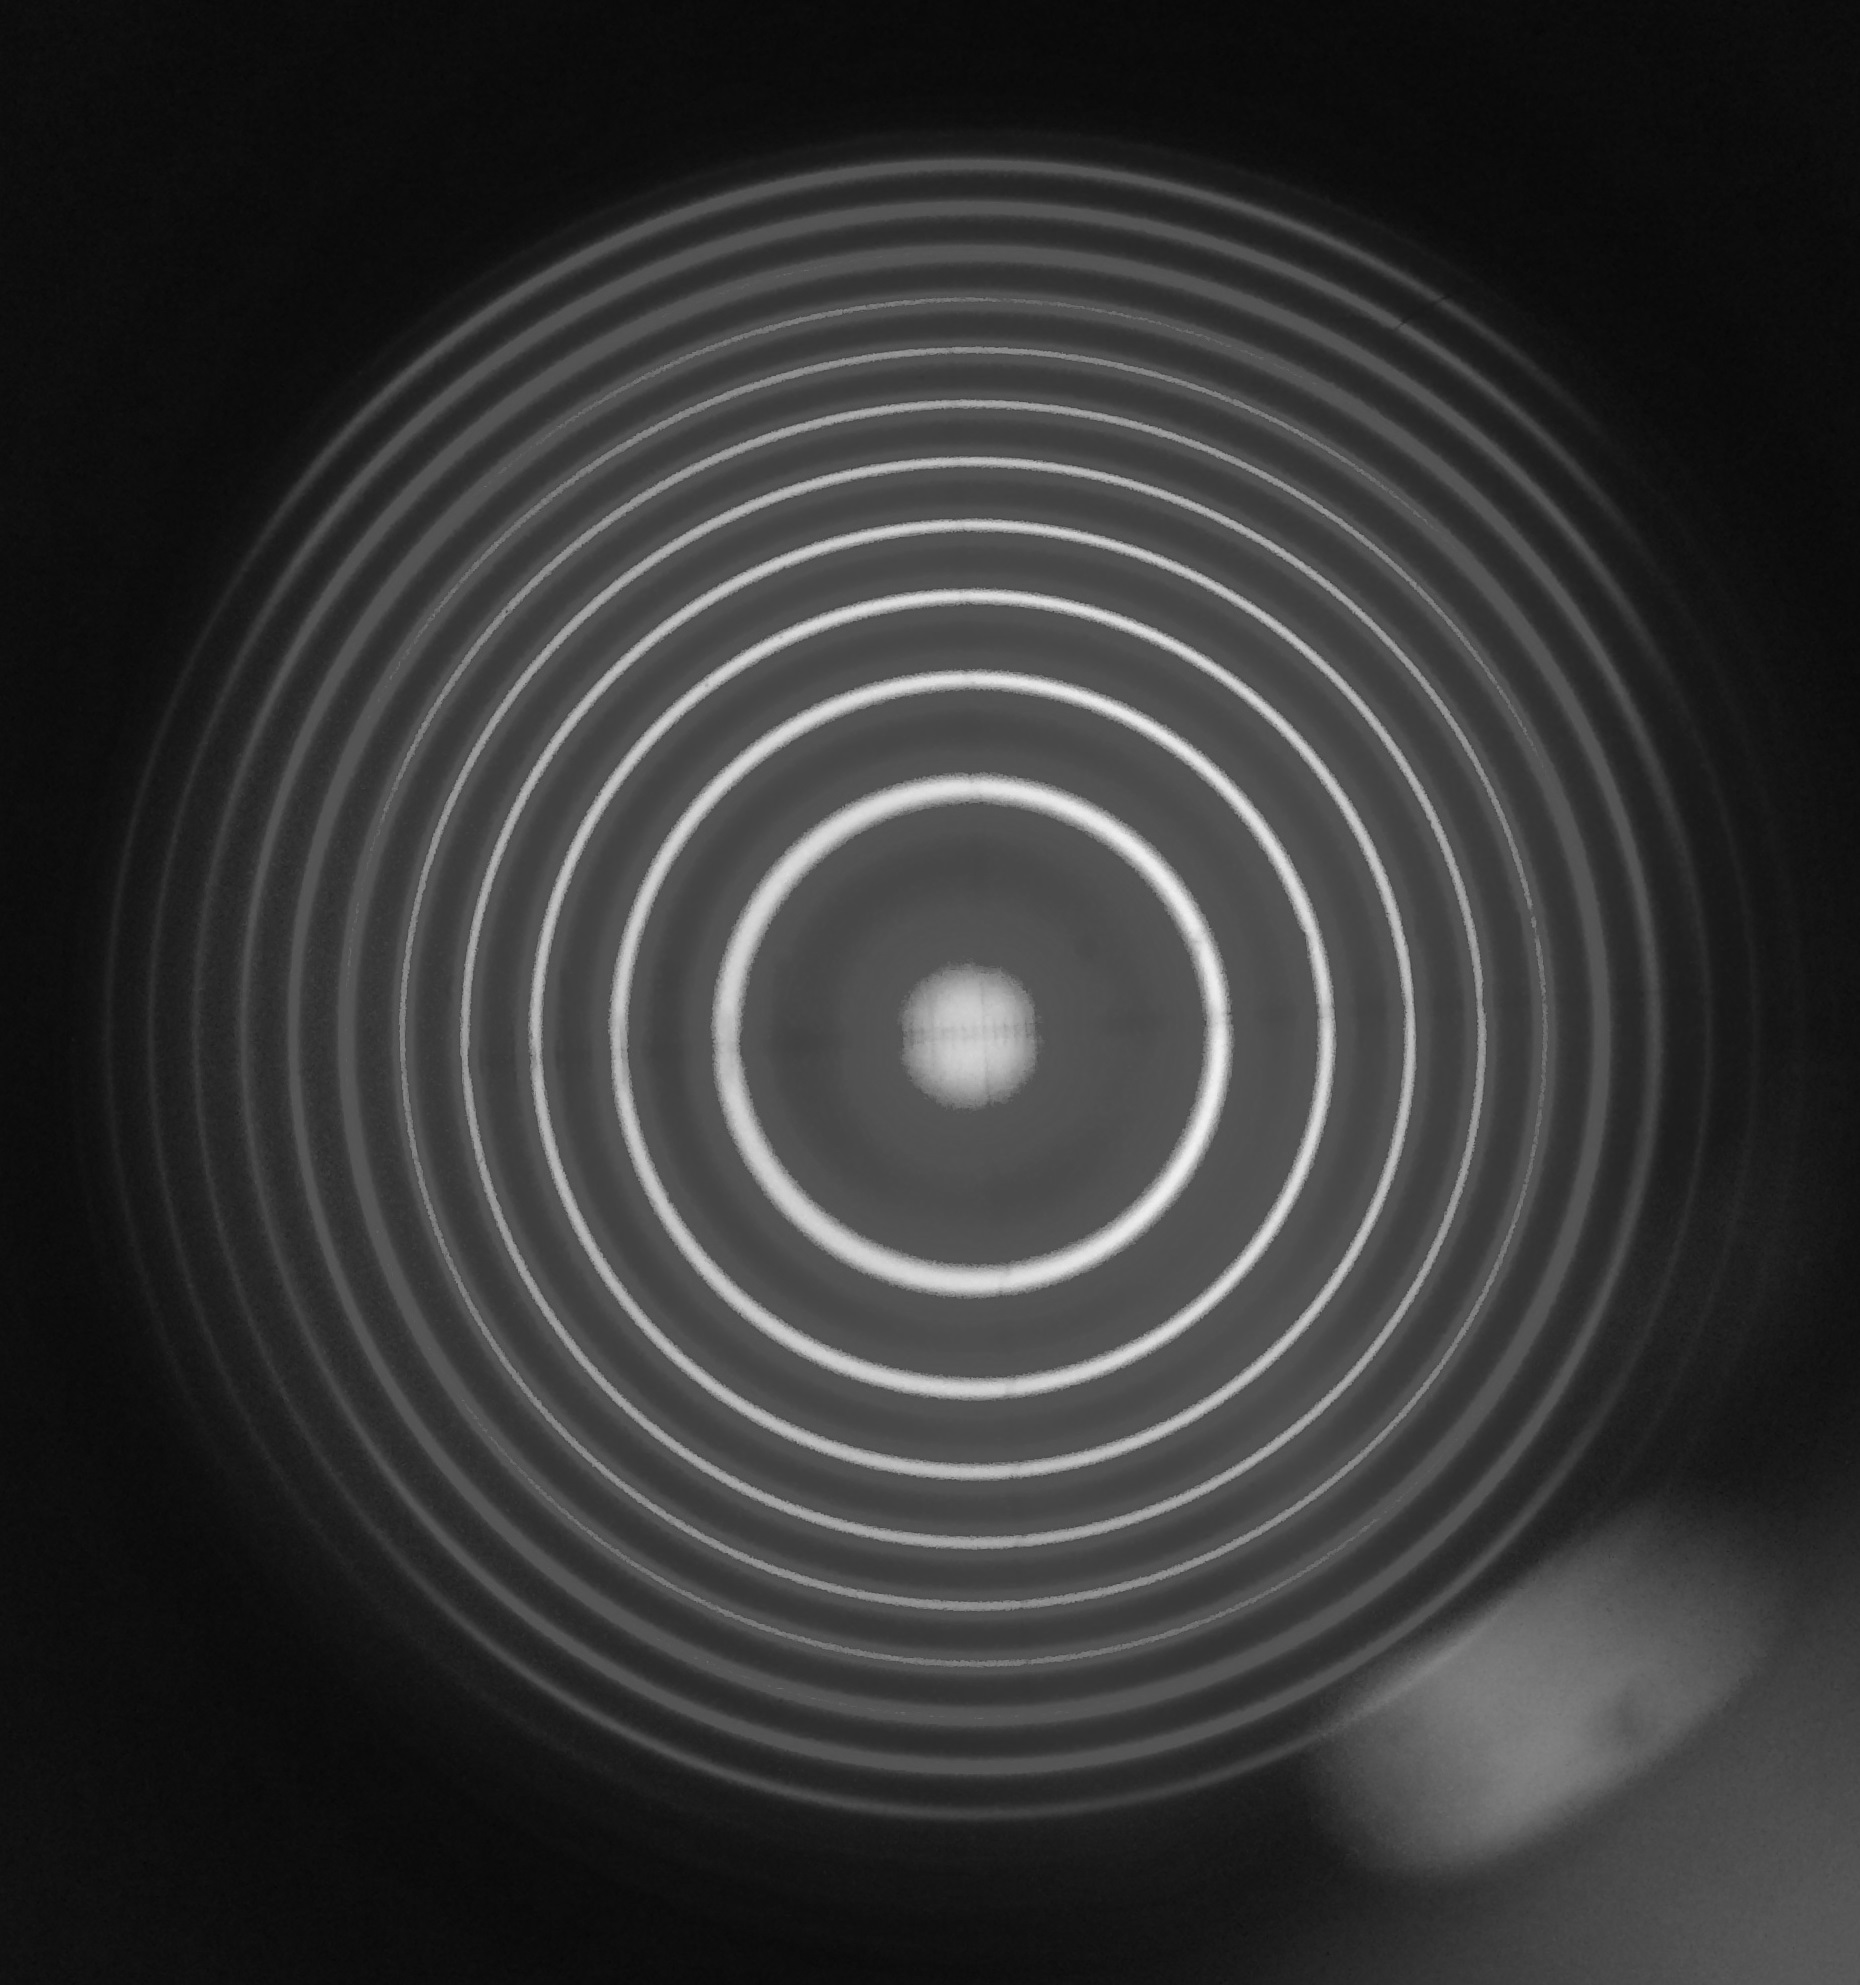
\includegraphics[width=0.7\textwidth]{data/bilder_okular/bild_1_edit.jpg}
    \subcaption{Interferenzmuster ohne Magnetfeld}
    \label{fig:bildtransohneB}
  \end{subfigure}%
  \begin{subfigure}[h]{0.5\textwidth}
    \centering
    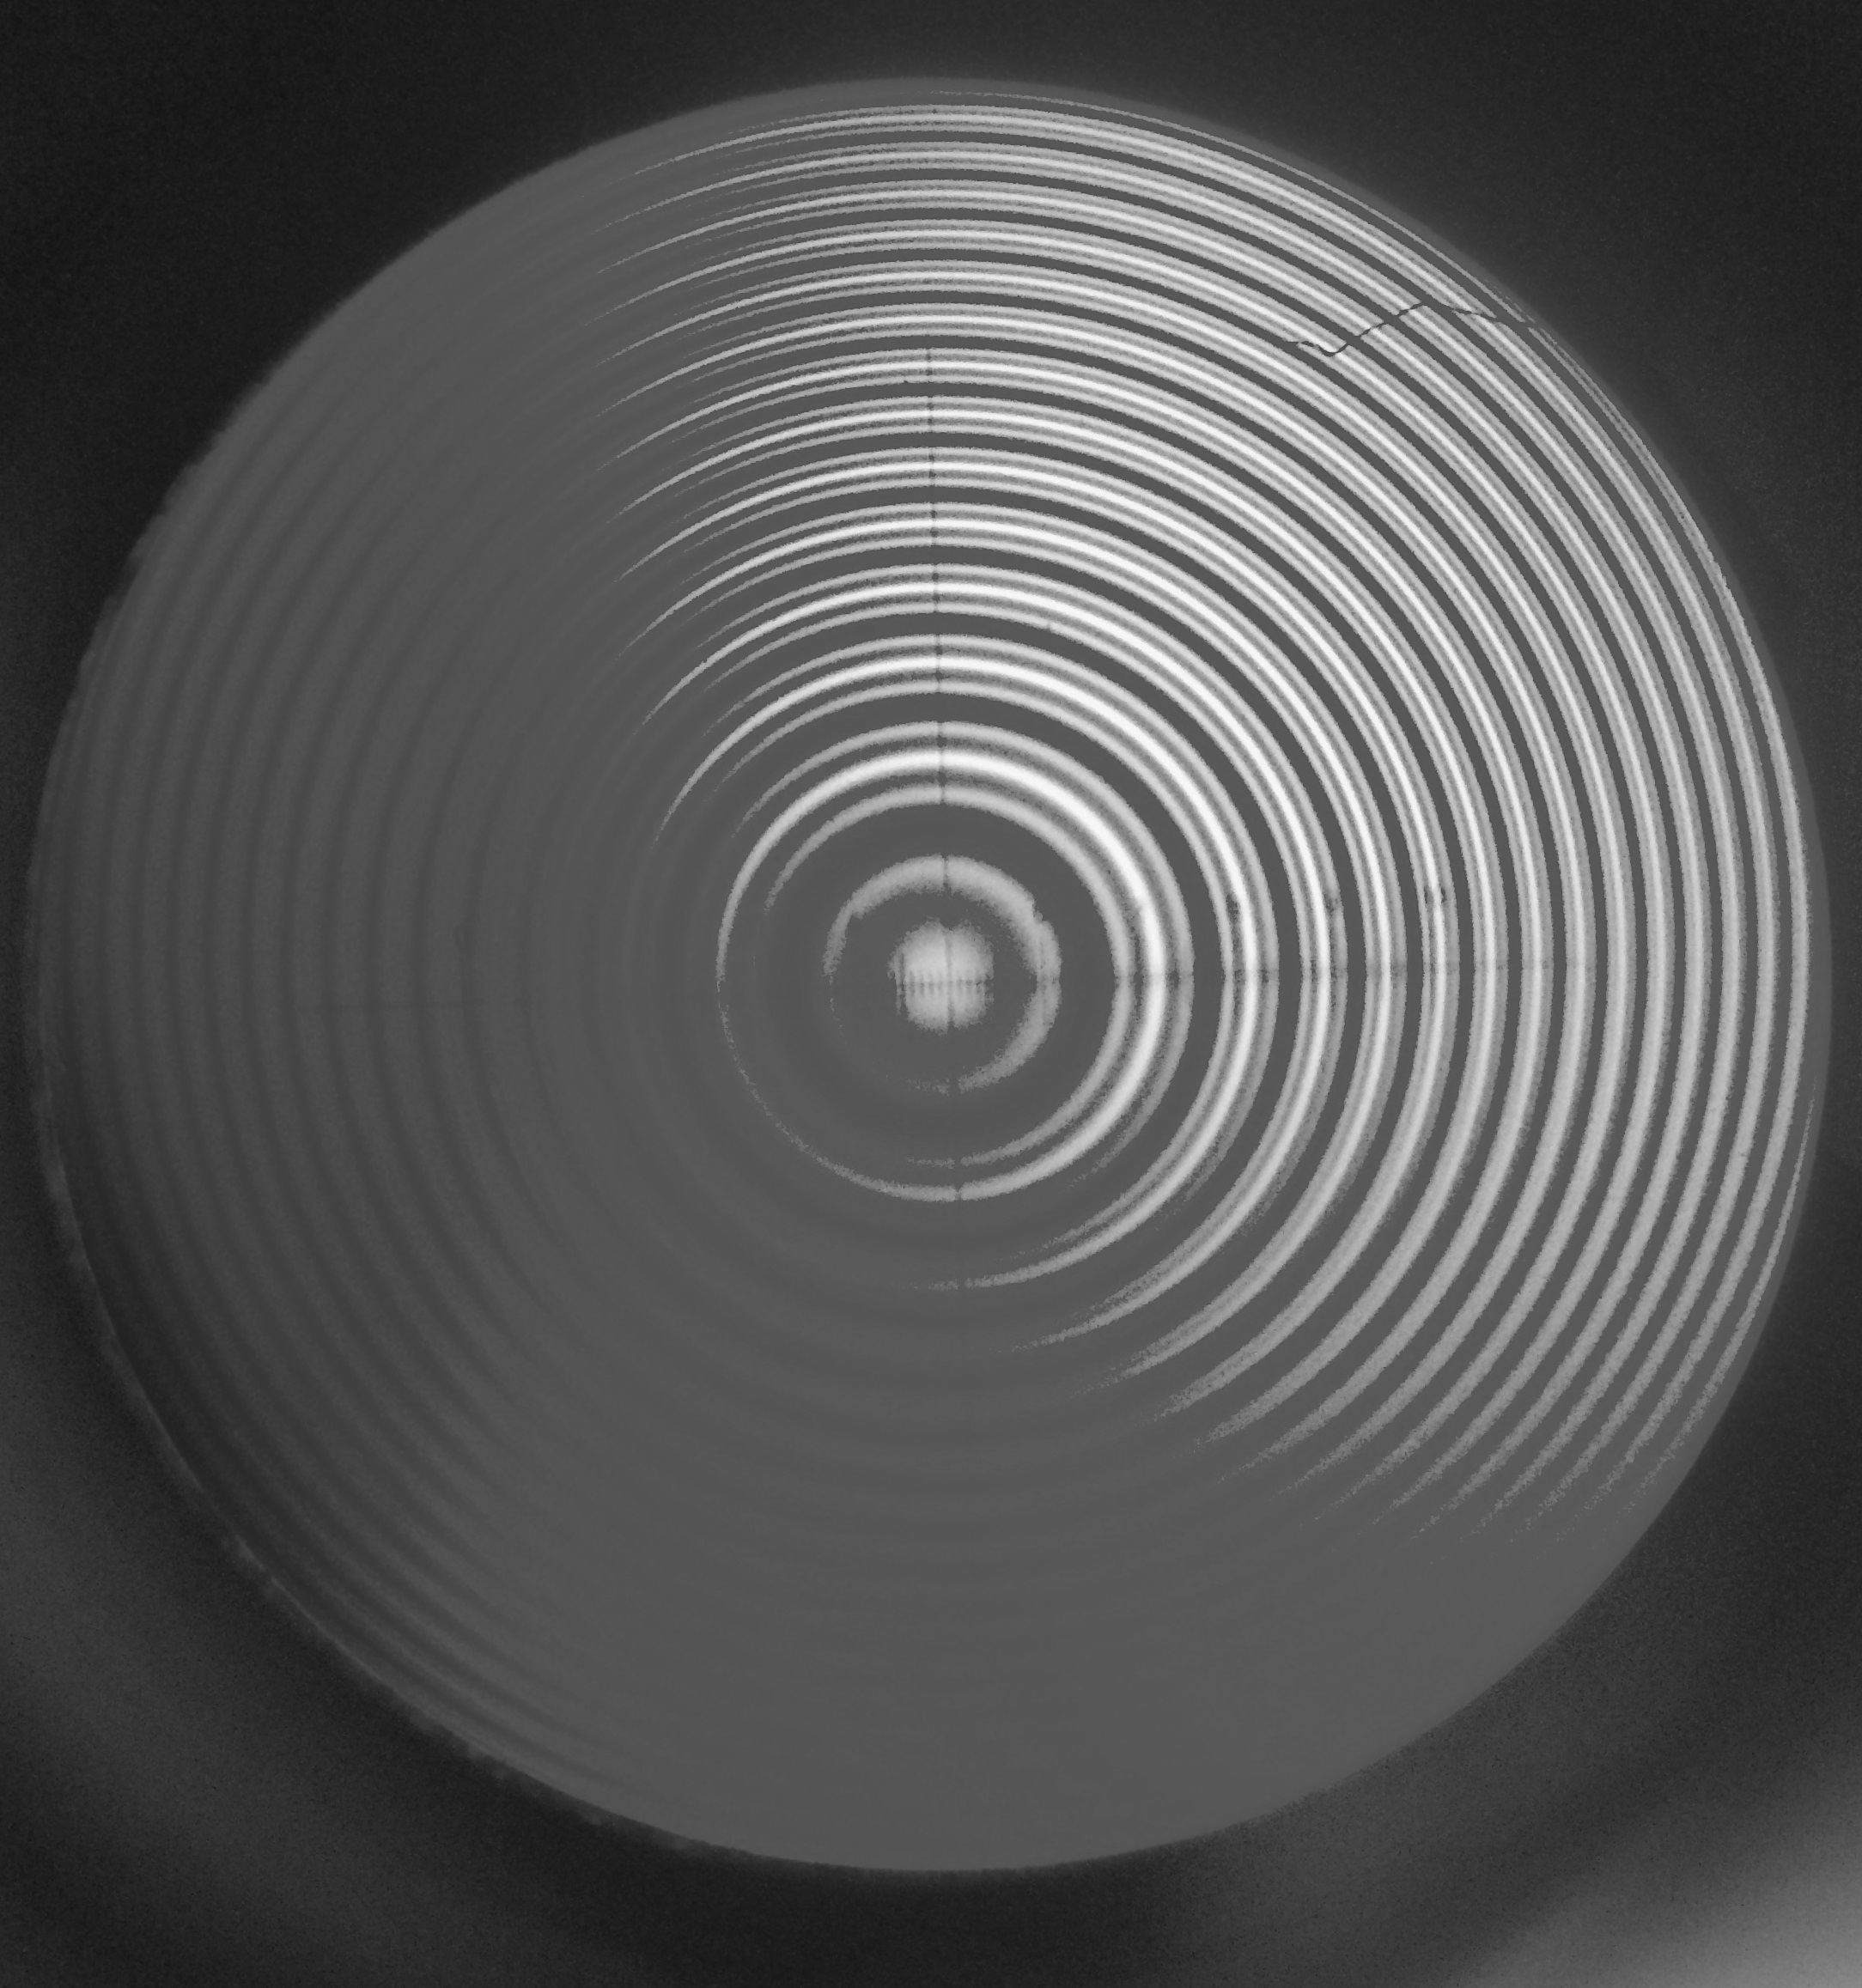
\includegraphics[width=0.7\textwidth]{data/bilder_okular/bild_2_edit.jpg}
    \subcaption{Interferenzmuster mit Magnetfeld $I=5,1\si{\ampere}$}
    \label{fig:bildtransmitB}
  \end{subfigure}
  \caption{}
\end{figure}

Stellt man einen Polarisationsfilter vor das Okular, so verschwinden unter dem Winkel von etwa $0^\circ$ zur Magnetfeldachse die $\sigma$-Komponenten (siehe Abb. \ref{fig:bildtransmitBsigma}). Das liegt daran, dass man in transversaler Richtung nur eine lineare Komponente der zirkular polarisierten Welle betrachtet, und diese somit verschwinden kann. Unter dem Winkel von $90^\circ$ verschwindet die $\pi$-Komponente (siehe Abb. \ref{fig:bildtransmitBpi}), dass bedeutet, dass das abgestrahlte $\pi$-Licht eine Polarisation in Magnetfeld-Richtung hat.\\
Bei einem Strom von $\si{(1,8\pm 0,1)\ampere}$ kann man die Linien gerade noch trennen.

\begin{figure}[h]
  \centering
  \begin{subfigure}[h]{0.5\textwidth}
    \centering
    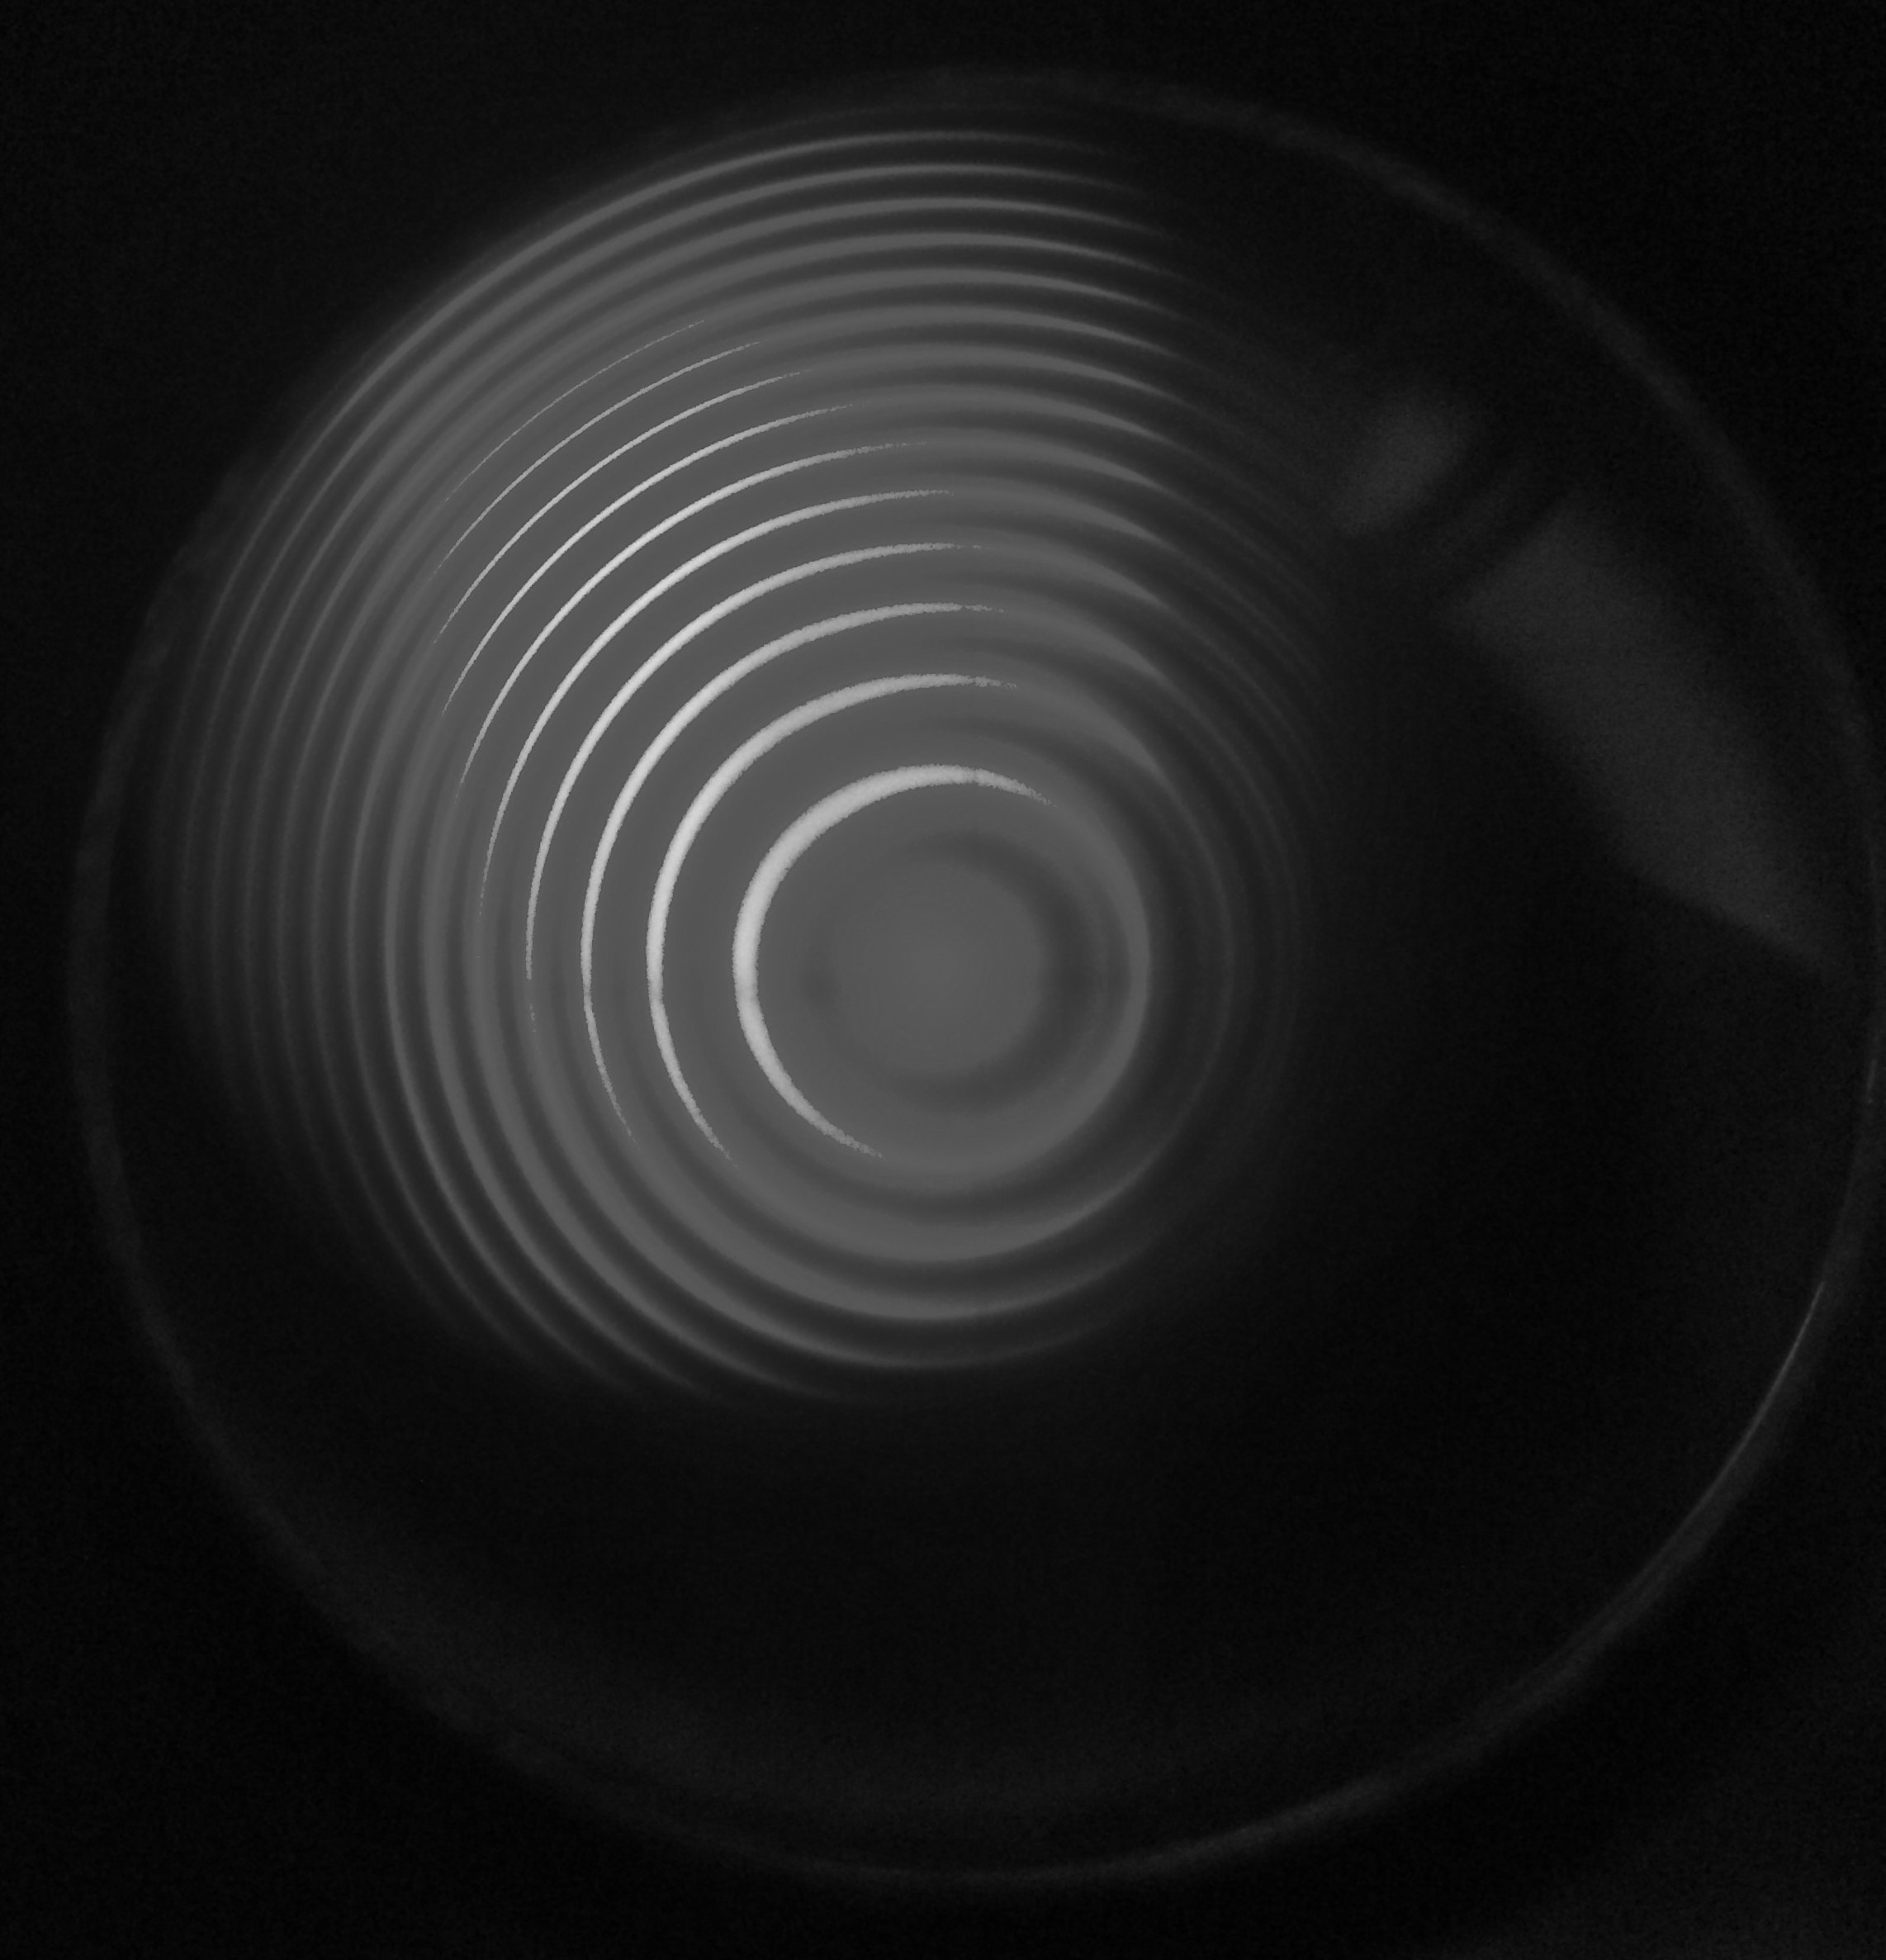
\includegraphics[width=0.7\textwidth]{data/bilder_okular/bild_3_edit.jpg}
    \subcaption{Interferenzmuster mit Magnetfeld ohne $\sigma$-Komponenten}
    \label{fig:bildtransmitBsigma}
  \end{subfigure}%
  \begin{subfigure}[h]{0.5\textwidth}
    \centering
    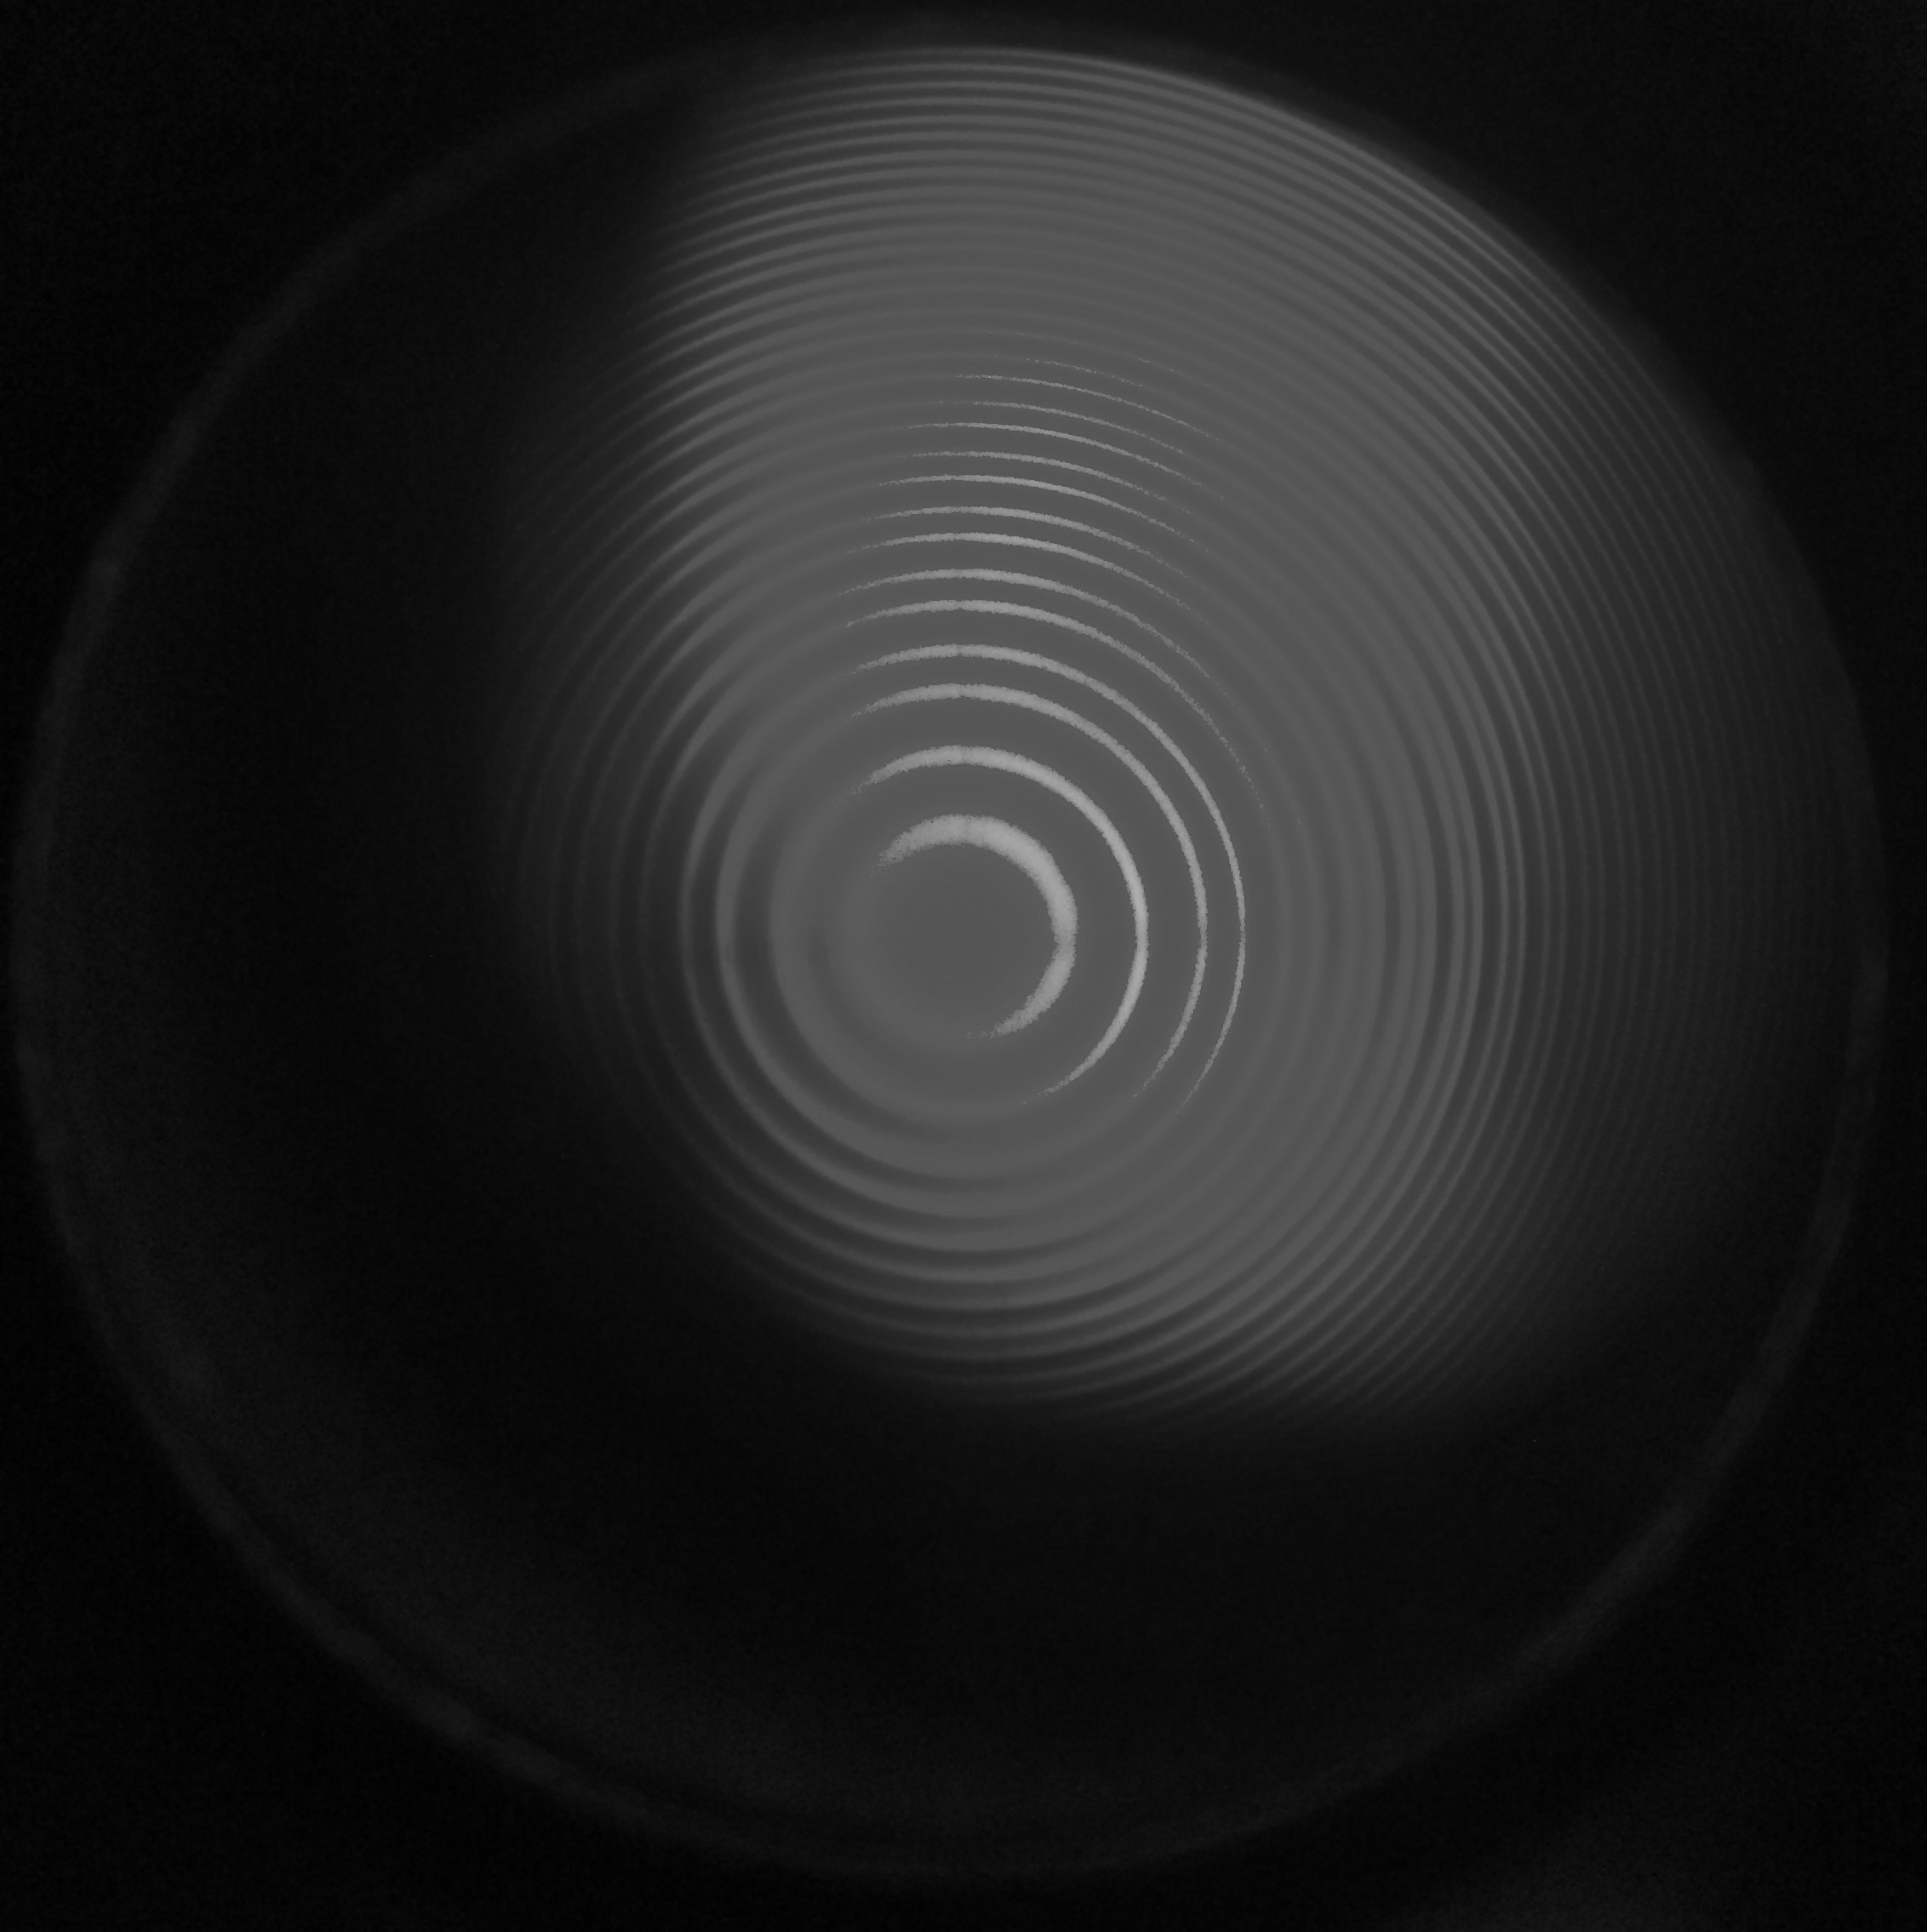
\includegraphics[width=0.7\textwidth]{data/bilder_okular/bild_4_edit.jpg}
    \subcaption{Interferenzmuster mit Magnetfeld ohne $\pi$-Komponente}
    \label{fig:bildtransmitBpi}
  \end{subfigure}
  \caption{}
\end{figure}

\paragraph{Longitudinale Konfiguration}
Betrachtet man das Interferenzmuster in longitudinaler Richtung, also in Richtung des Magnetfeldes, so ist ohne Magnetfeld (siehe Abb. \ref{fig:bildlongohneB}) kein Unterschied zu erkennen. Wenn man das Magnetfeld hochfährt (siehe Abb. \ref{fig:bildlongmitB}) spalten sich die Linien wieder auf. Allerdings sind diesmal nur 2 Kreise zu sehen, der mittlere fehlt. Das liegt daran, dass die $\pi$-Komponente nicht in Magnetfeldrichtung emittiert wird.

\begin{figure}[h]
  \centering
  \begin{subfigure}[h]{0.5\textwidth}
    \centering
    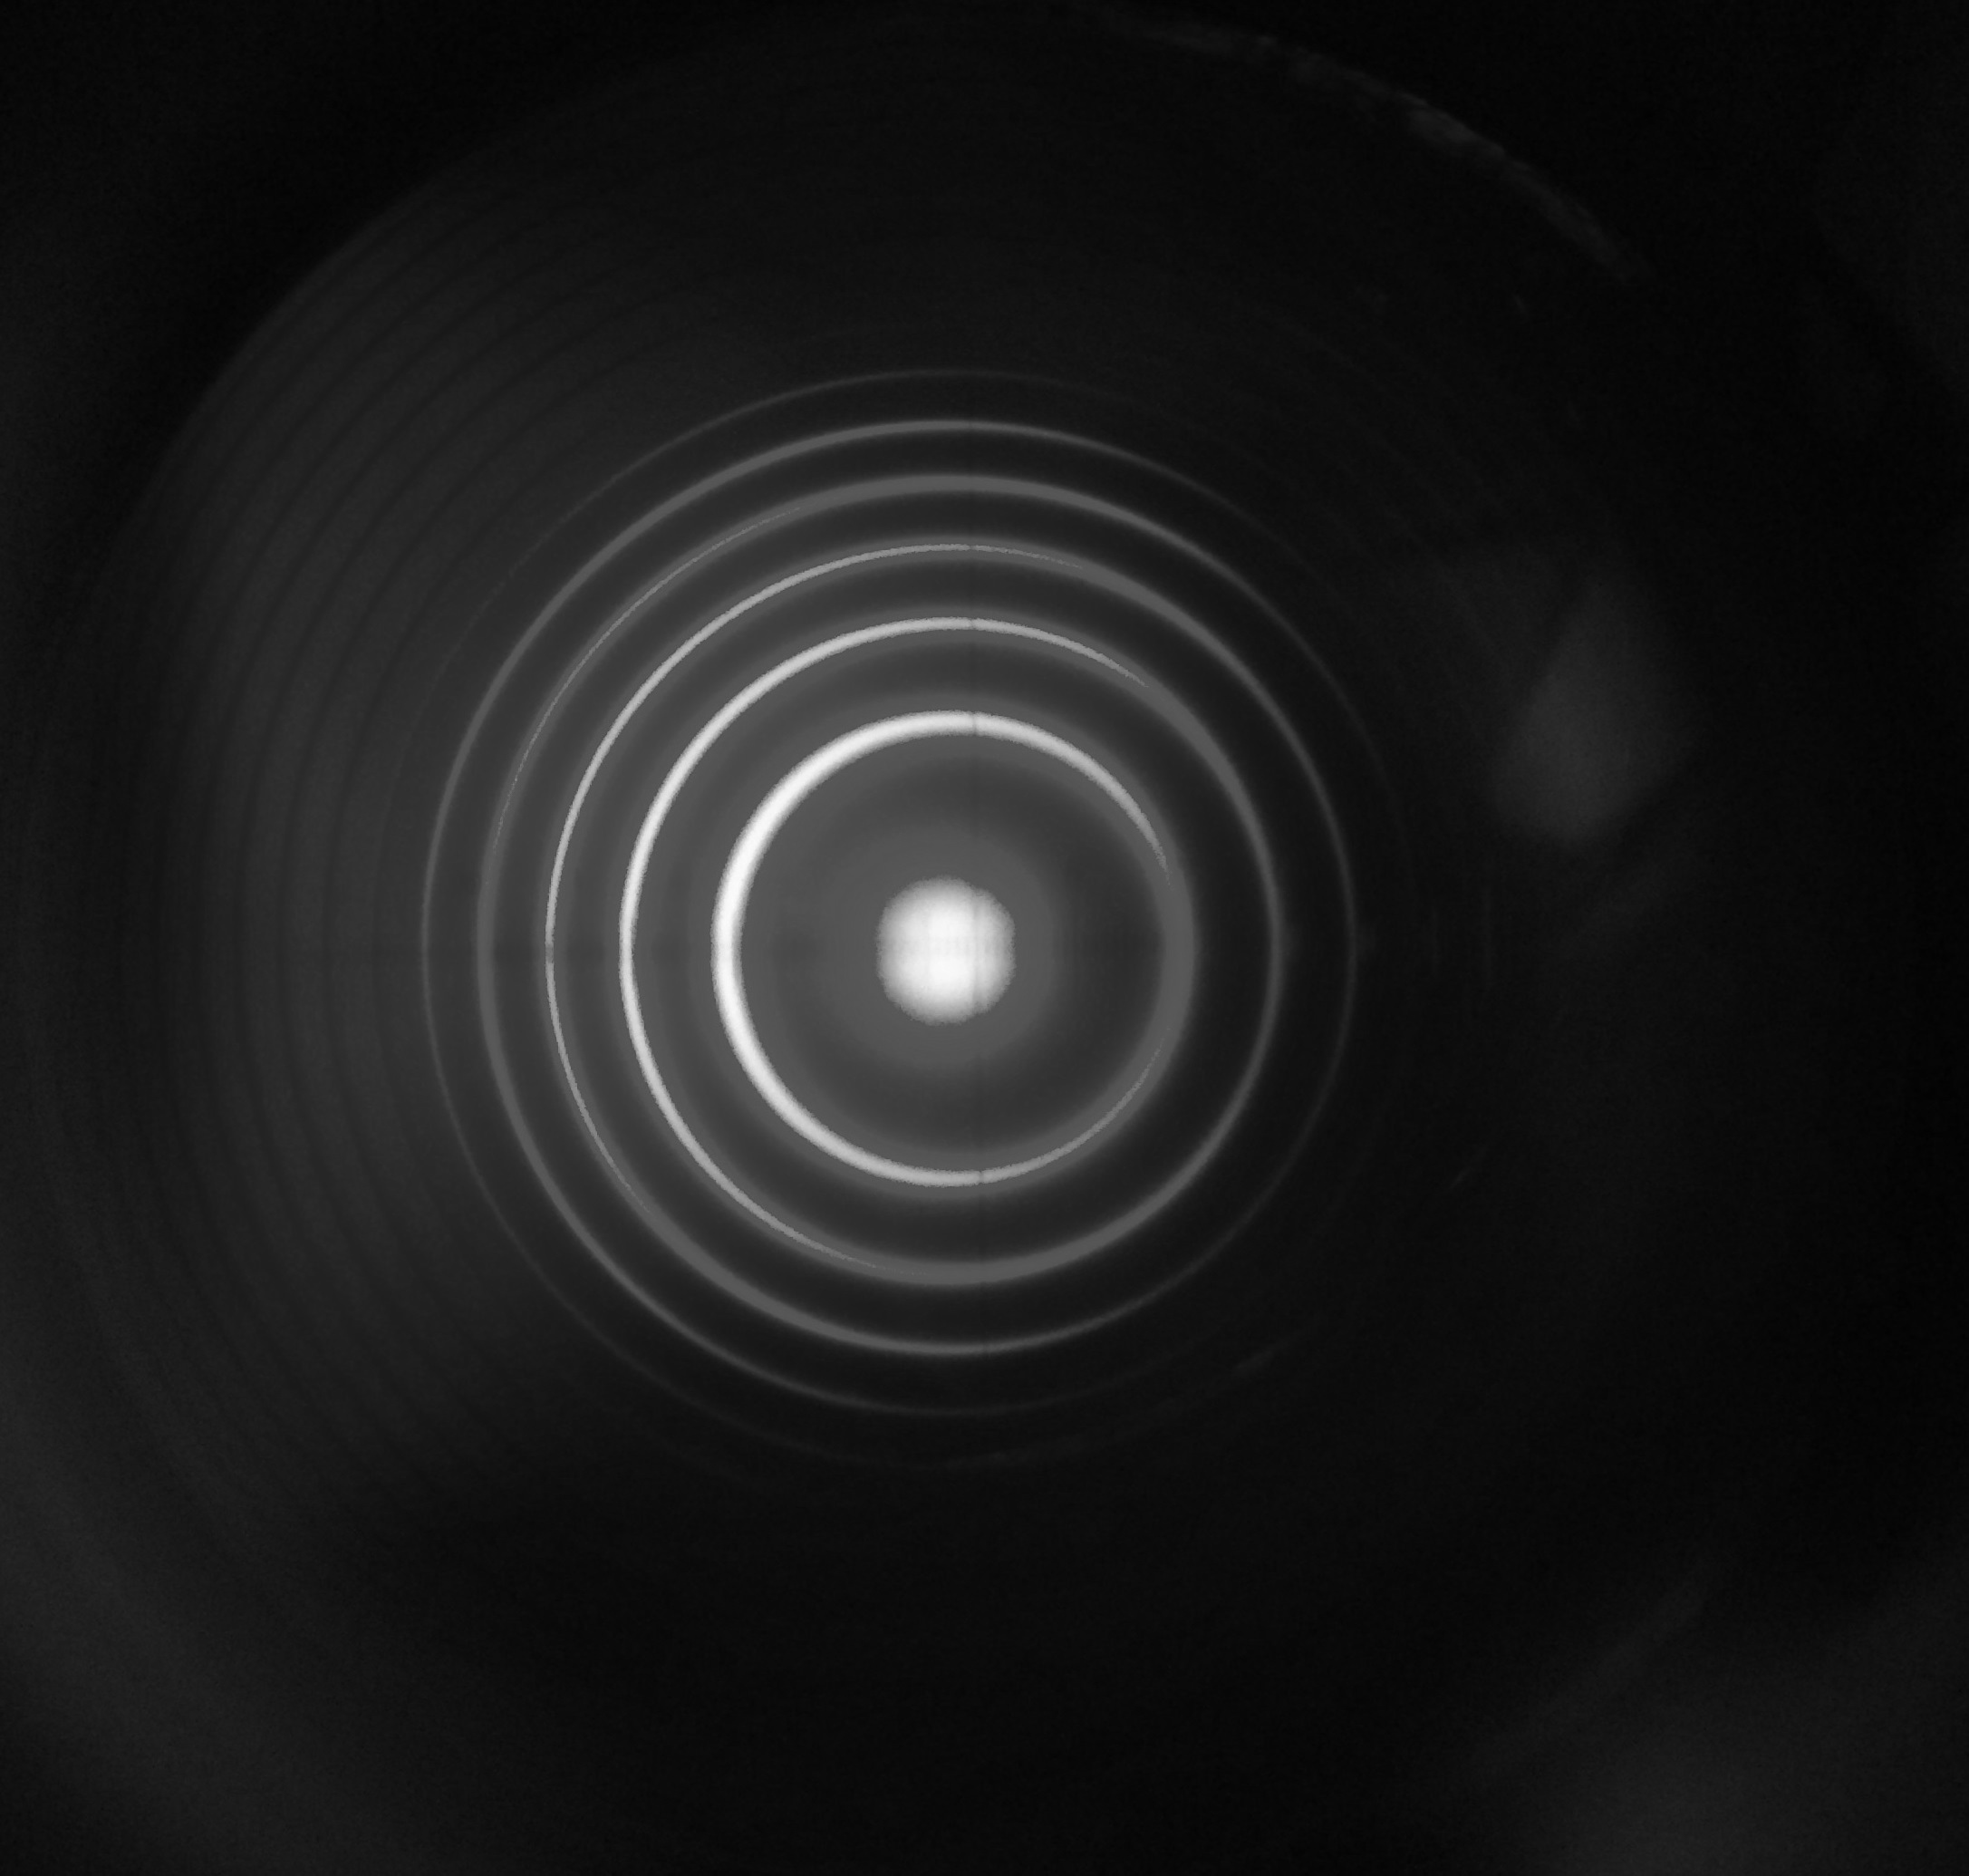
\includegraphics[width=0.7\textwidth]{data/bilder_okular/bild_5_edit.jpg}
    \subcaption{Interferenzmuster ohne Magnetfeld}
    \label{fig:bildlongohneB}
  \end{subfigure}%
  \begin{subfigure}[h]{0.5\textwidth}
    \centering
    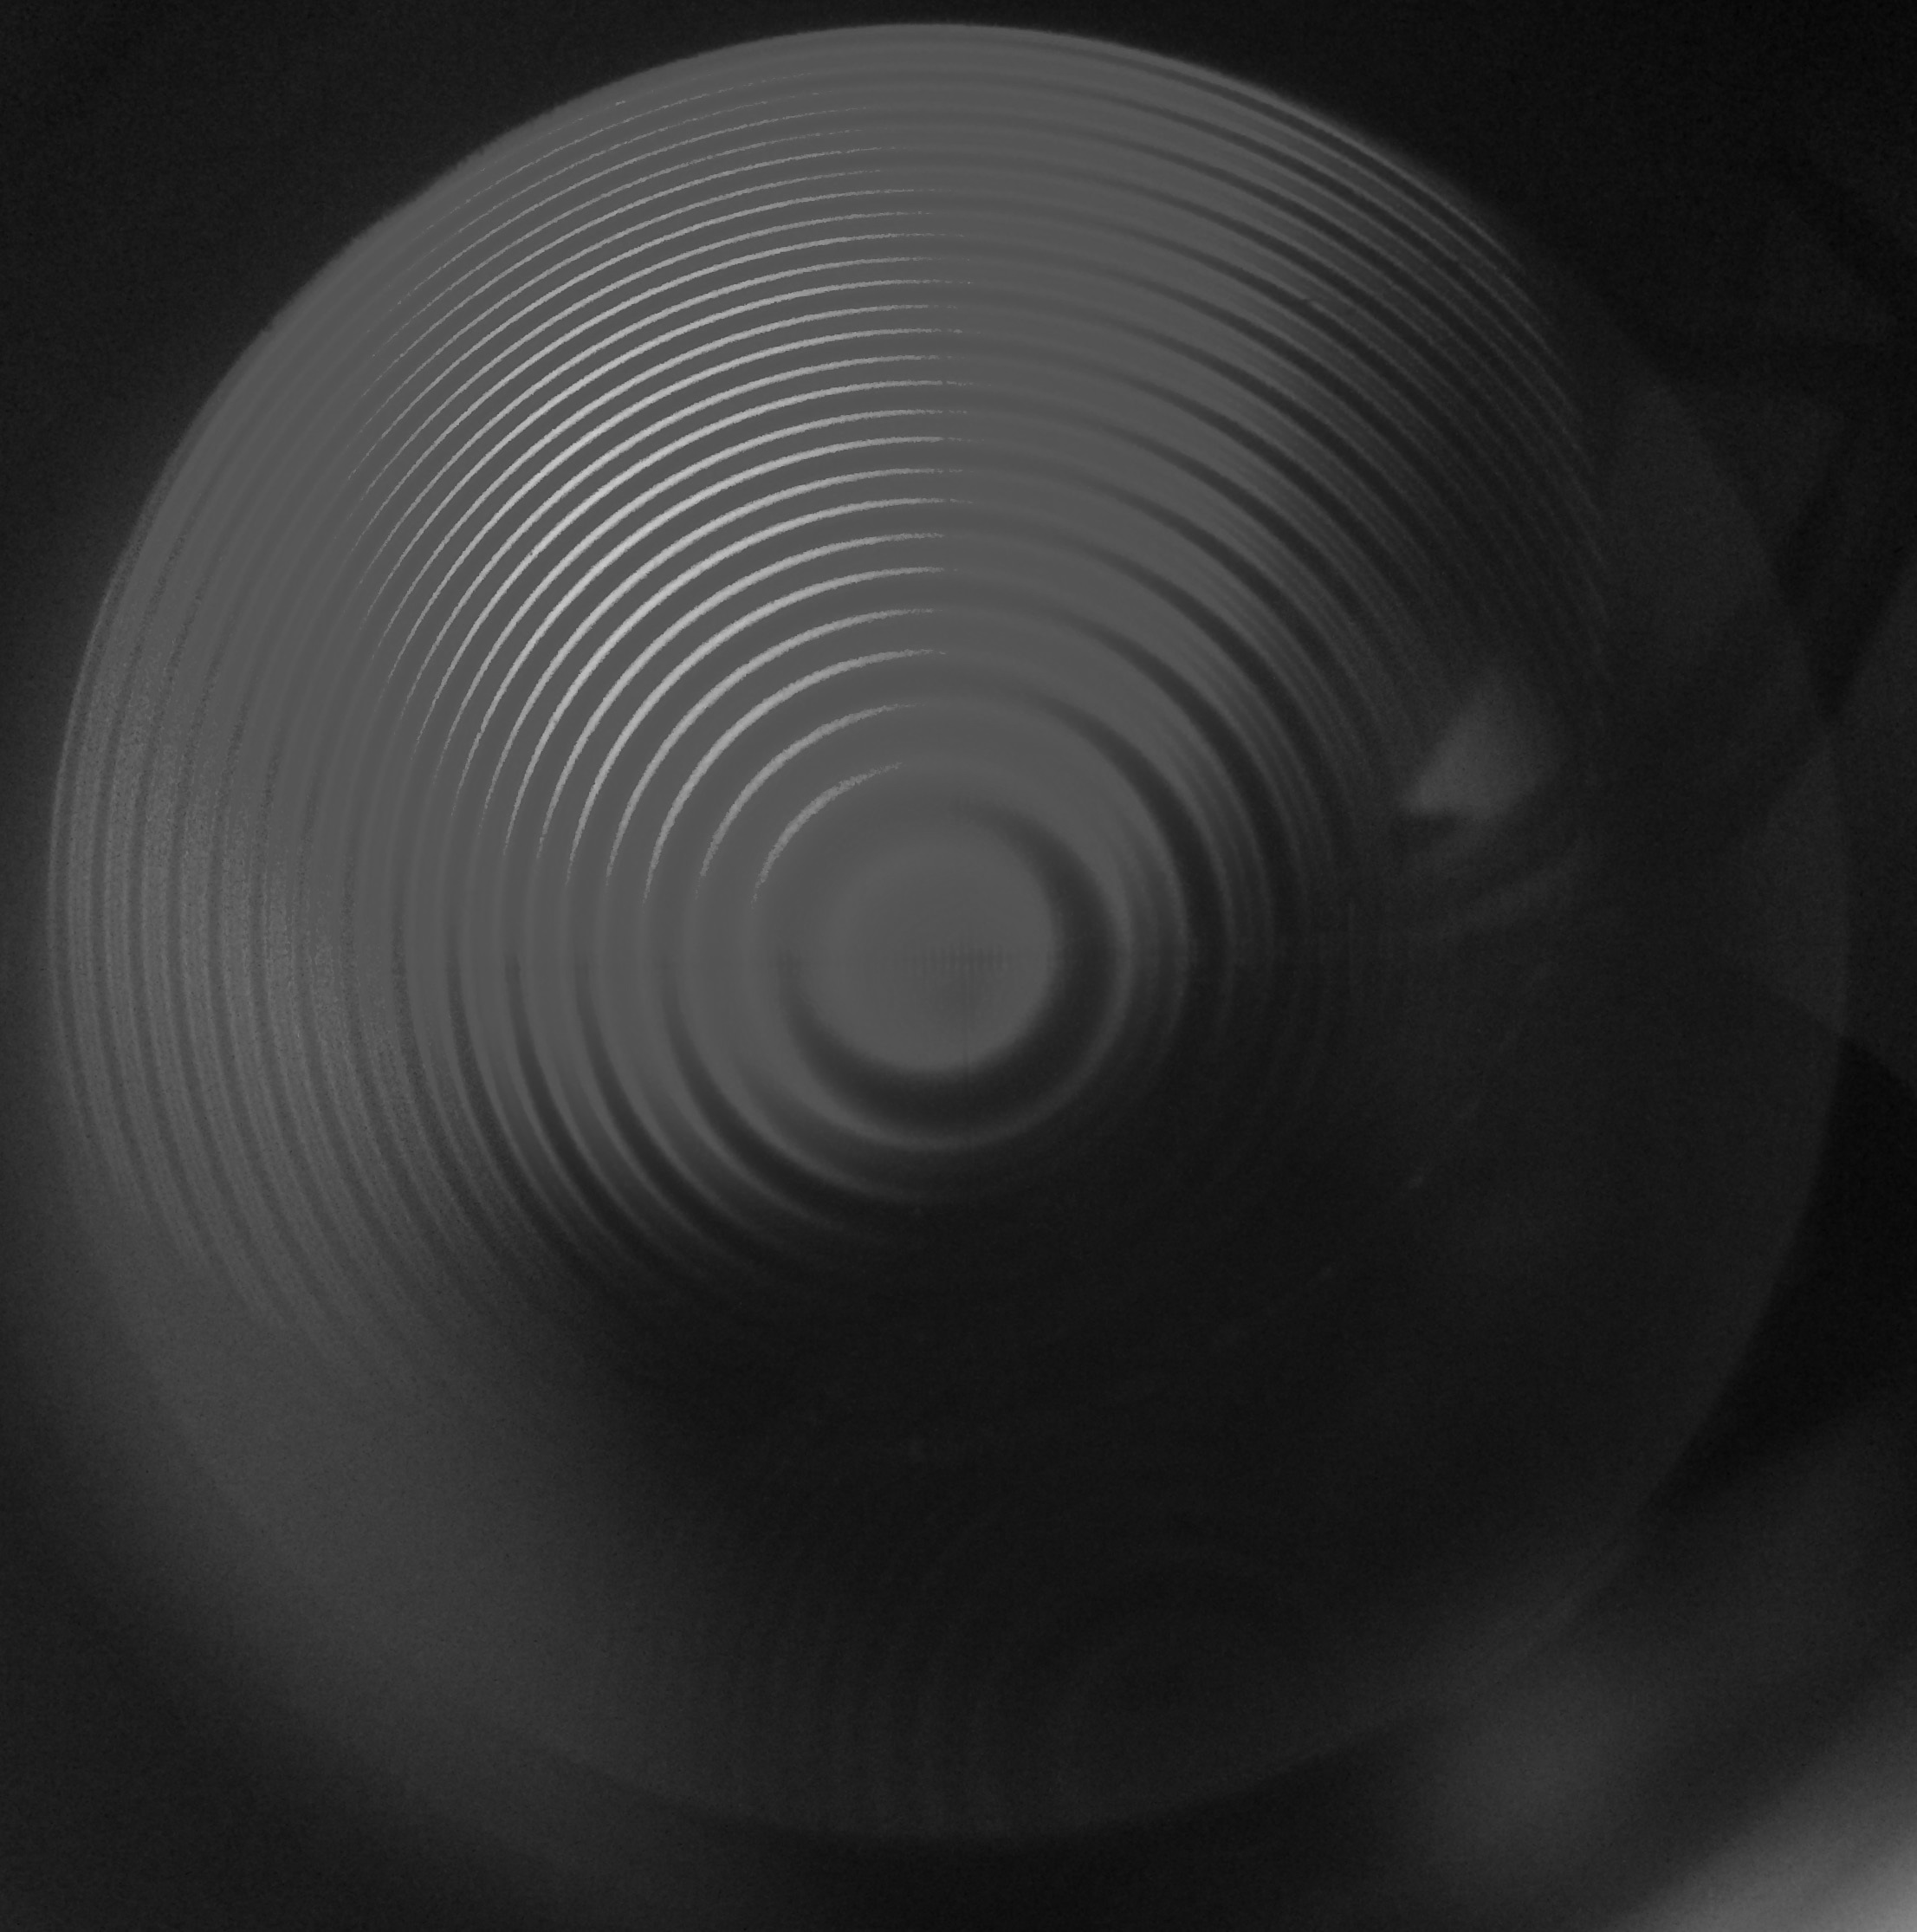
\includegraphics[width=0.7\textwidth]{data/bilder_okular/bild_6_edit.jpg}
    \subcaption{Interferenzmuster mit Magnetfeld $I=5,1\si{\ampere}$}
    \label{fig:bildlongmitB}
  \end{subfigure}
  \caption{}
\end{figure}

\begin{figure}[h]
  \centering
  \begin{subfigure}[h]{0.5\textwidth}
    \centering
    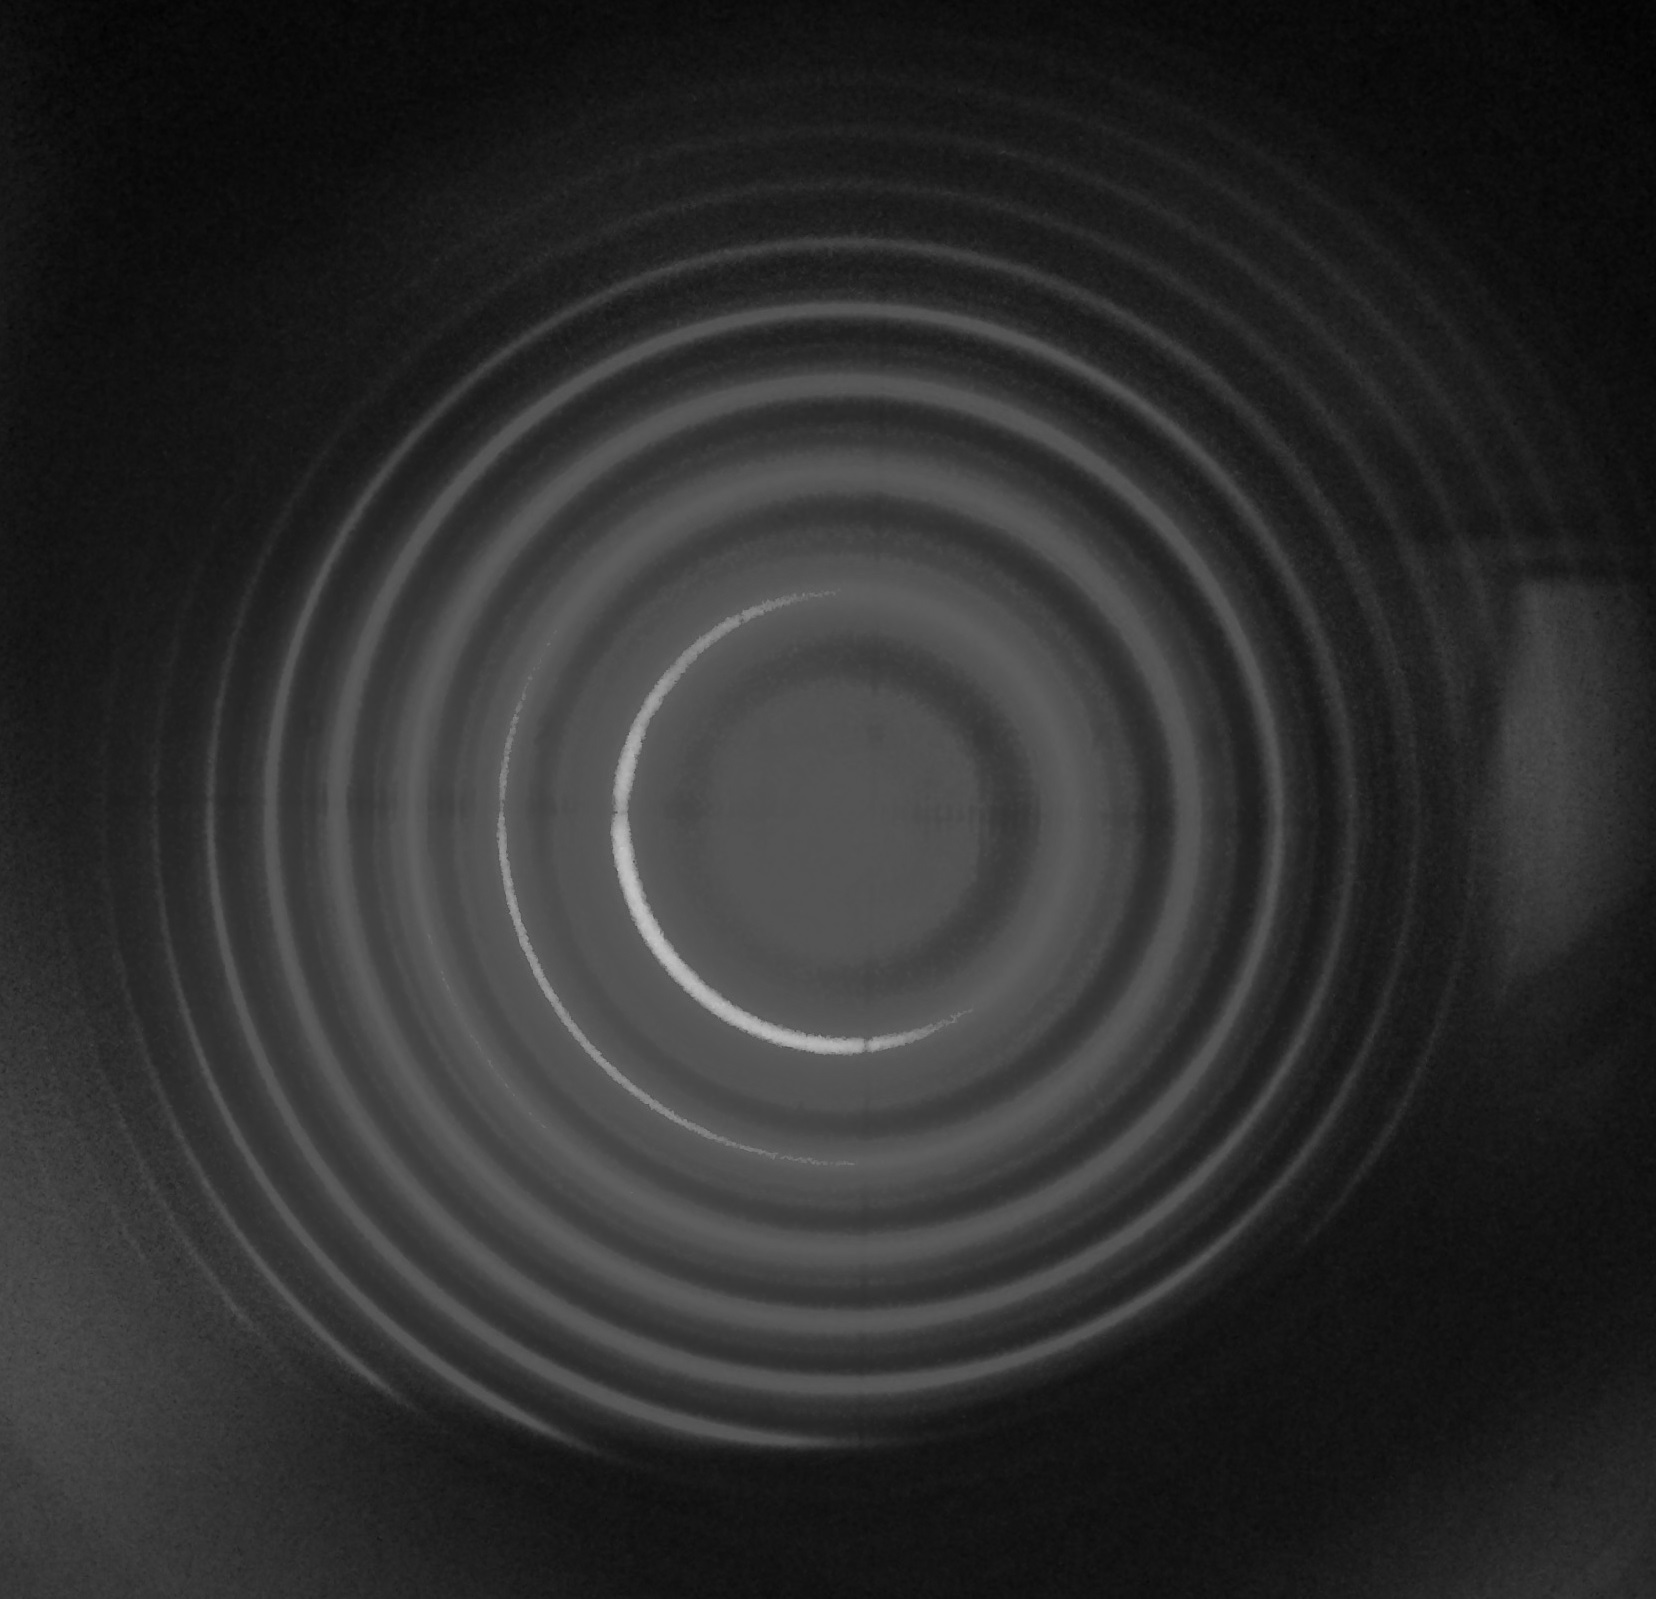
\includegraphics[width=0.7\textwidth]{data/bilder_okular/bild_7_edit.jpg}
    \subcaption{Interferenzmuster mit Magnetfeld ohne $\sigma^+$-Komponenten}
    \label{fig:bildlongmitBsigmaplus}
  \end{subfigure}%
  \begin{subfigure}[h]{0.5\textwidth}
    \centering
    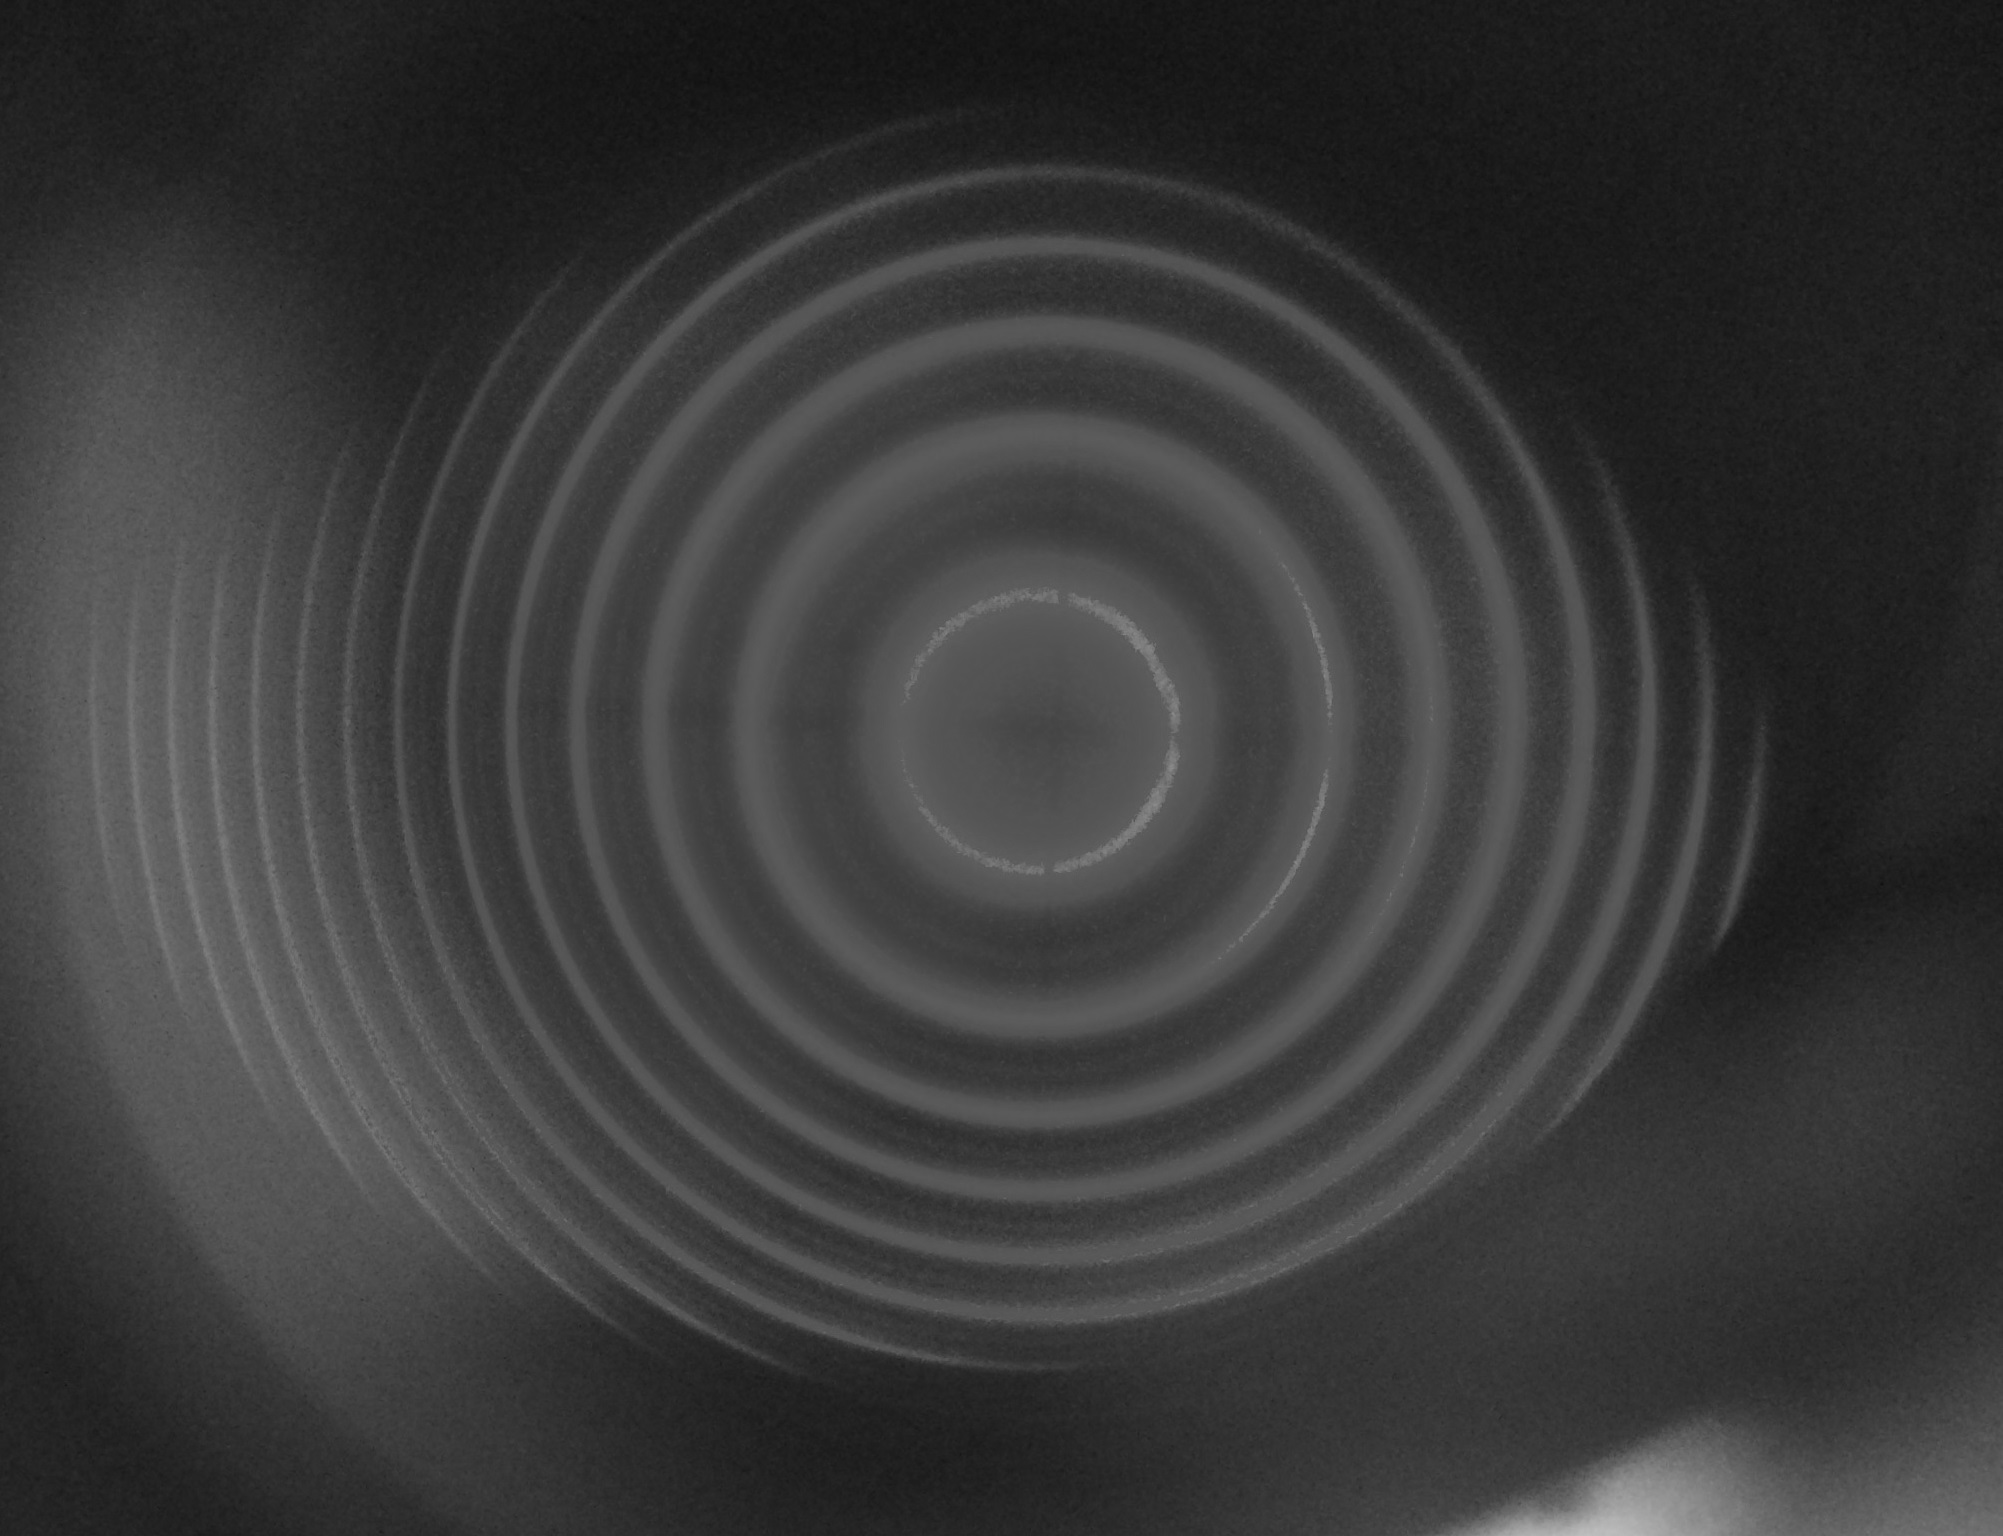
\includegraphics[width=0.9\textwidth]{data/bilder_okular/bild_8_edit.jpg}
    \subcaption{Interferenzmuster mit Magnetfeld ohne $\sigma^-$-Komponente}
    \label{fig:bildlongmitBsigmaminus}
  \end{subfigure}
  \caption{}
\end{figure}

Stellt man ein $\lambda/4$-Plättchen und einen Polarisationsfilter vor das Okular, so verschwinden unter dem Winkel von etwa $(-44 \pm 5)^\circ$ zur optischen Achse des $\lambda/4$-Plättchens die äußere ($\sigma^+$) Komponente (siehe Abb. \ref{fig:bildlongmitBsigmaplus}) und unter einem Winkel von $(43 \pm 5)^\circ$ die innere ($\sigma^-$) Komponente (siehe Abb. \ref{fig:bildlongmitBsigmaminus}). Demzufolge handelt es sich wirklich um zirkular polarisiertes Licht. Beides ist in den Abbildungen leider nicht sehr gut zu erkennen.\\
Bei einem Strom von $\si{(1,1\pm 0,1)\ampere}$ kann man die Linien gerade noch trennen.
\newpage
\subsubsection{Messung des Zeeman-Effektes}
\paragraph{Kalibrierung}
In Abb. \ref{fig:kal_raw} sind die aufgenommenen Kalibrierungskurven dargestellt. Für das Experiment haben wir nur den Bereich $6,0\si{\ampere} - 8,5\si{\ampere}$ benötigt. Man kann erkennen, dass sie sich leicht unterscheiden. Deswegen fitten wir an die Kurven in diesem Bereich jeweils eine quadratische Funktion $B = a\cdot I^2 + b \cdot I + c$ (siehe Abb. \ref{fig:kal_raw_edit}). Die Fitparameter unterscheiden sich natürlich für beide Kurven. Da wir keine Aussage darüber treffen können, welche Kurve man eher verwenden sollte, haben wir uns dazu entschlossen, die Mittelwerte der Parameter $p = \frac{p_1+p_2}{2} , \Delta p = \frac{p_1-p_2}{2}$ ($p = a,b,c$) als Parameter zu wählen. Es ergibt sich: 
\begin{align*}
a &= \si{(-6,8 \pm 0,5)\tesla\ampere^{-2}}\\
b &= \si{(142 \pm 10) \tesla\ampere^{-1}}\\
c &= \si{(-91 \pm 50)\tesla}
\end{align*}

Im folgendem Berechnen wir das Magnetfeld aus dem Strom ($\Delta I = \si{0,1 \ampere}$) über:
\begin{align*}
B &= a\cdot I^2 + b \cdot I + c\\
\Delta B &= \sqrt{(I^2\Delta a)^2 + (I \Delta b)^2 + \Delta c^2 + ((2aI+b)\Delta I)^2}
\end{align*}

\begin{figure}[h]
  \centering
  \begin{subfigure}[h]{0.5\textwidth}
    \centering
    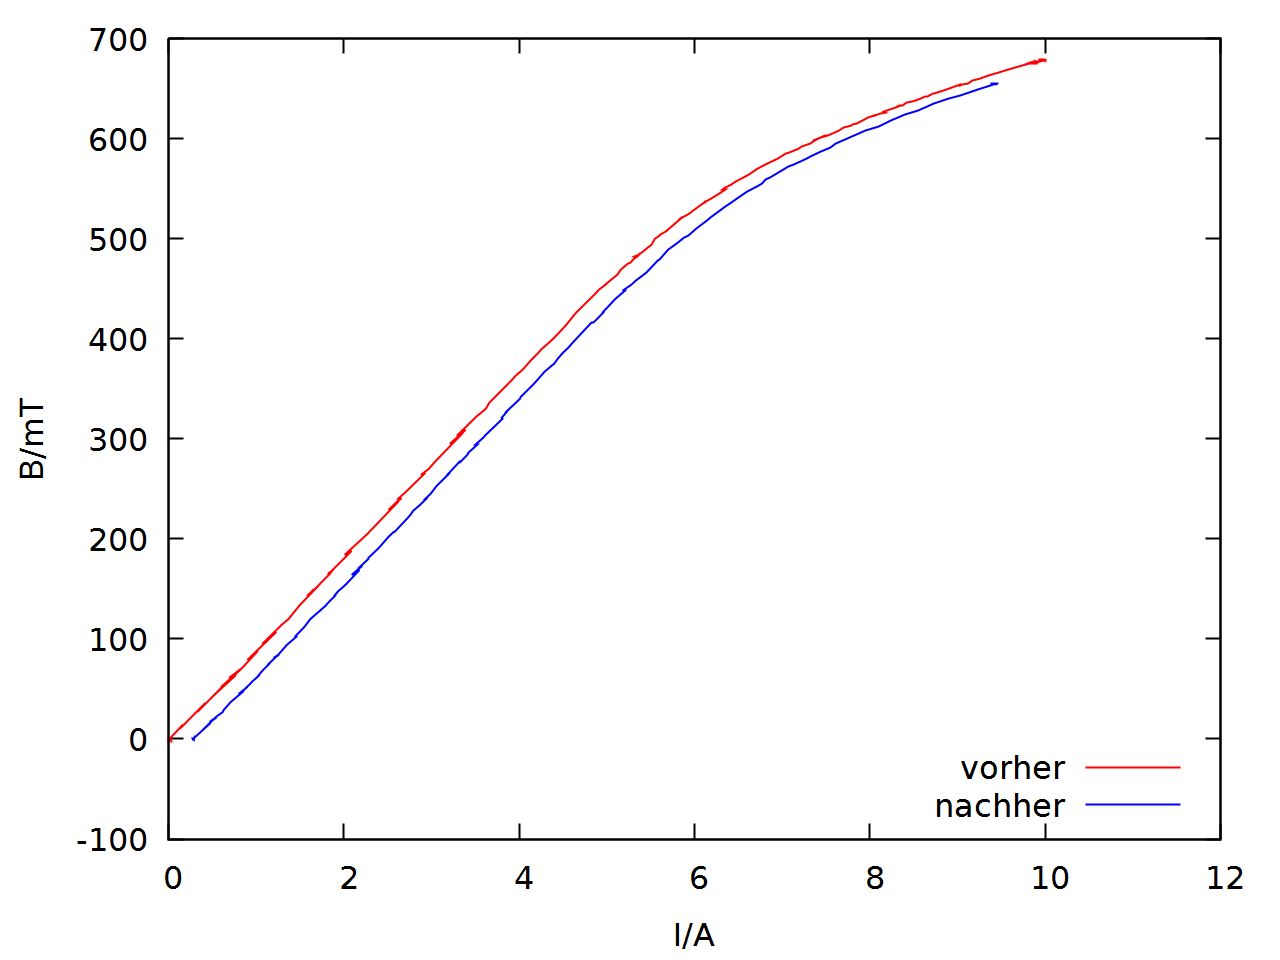
\includegraphics[width=0.9\textwidth]{data/zeeman/out_kalibrierung.png}
    \subcaption{Aufgenommene Kalibrierungskurve}
    \label{fig:kal_raw}
  \end{subfigure}%
  \begin{subfigure}[h]{0.5\textwidth}
    \centering
    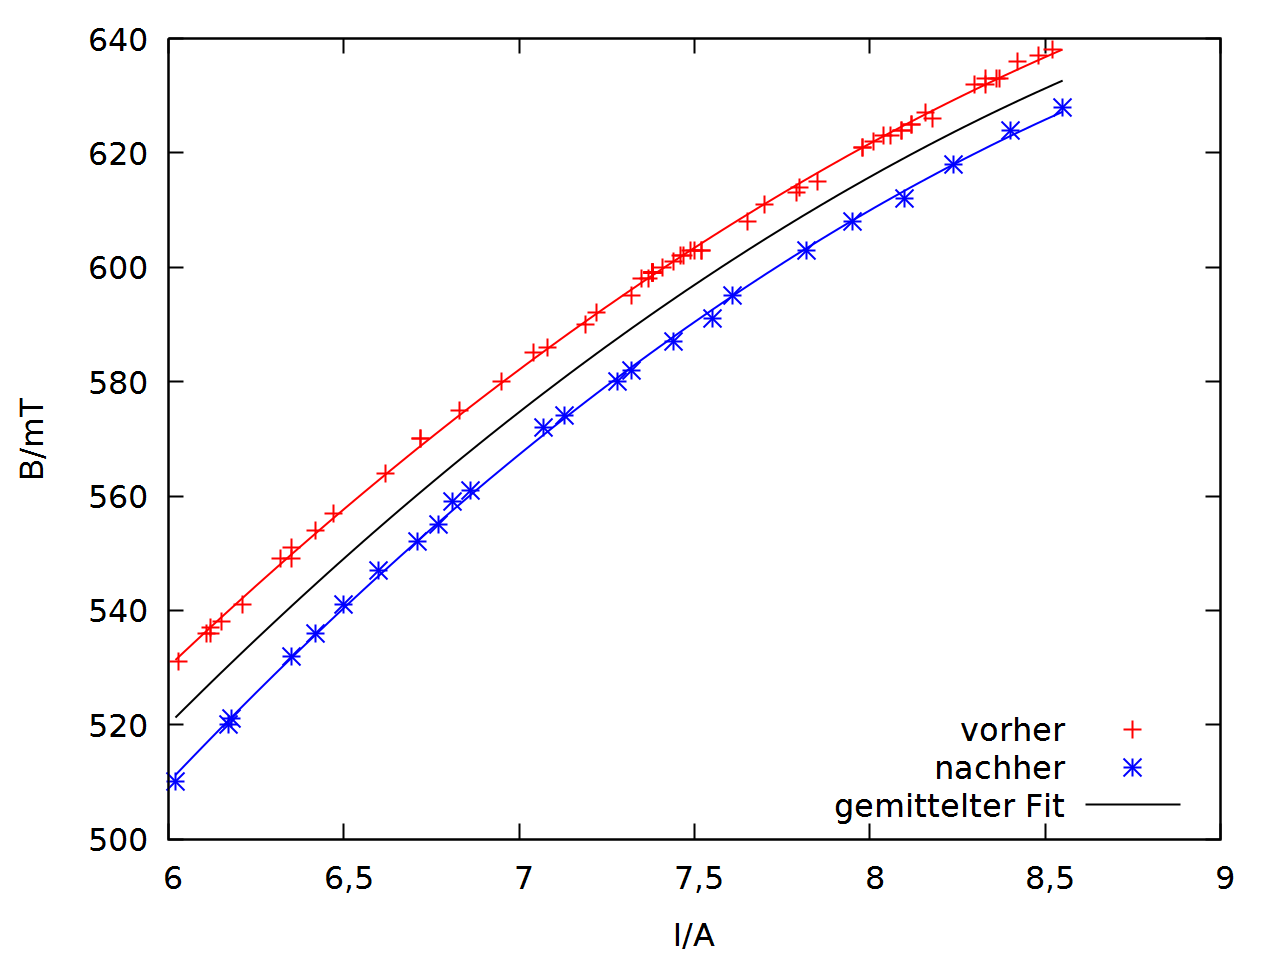
\includegraphics[width=0.9\textwidth]{data/zeeman/out_kalibrierung_edit.png}
    \subcaption{Fit an die Kalibrierungskurve}
    \label{fig:kal_raw_edit}
  \end{subfigure}
  \caption{Kalibrationskurven für das Magnetfeld}
\end{figure}

\paragraph{Messwerte}
Die Aufspaltung konnte man mit der CCD-Kamera ab etwa $6\si{\ampere}$ beobachten (siehe Abb. \ref{fig:raw_1} und \ref{fig:raw}). Wir erhöhten danach den Strom in $0,3\si{\ampere}$-Schritten. Die Stromquelle erhöhte allerdings nach $8,5\si{\ampere}$ den Strom nicht weiter, so dass wir nur Daten aus dem Bereich $6\si{\ampere}-8,5\si{\ampere}$ haben.
\begin{figure}[!h]
\centering
\begin{subfigure}{0.45\textwidth}
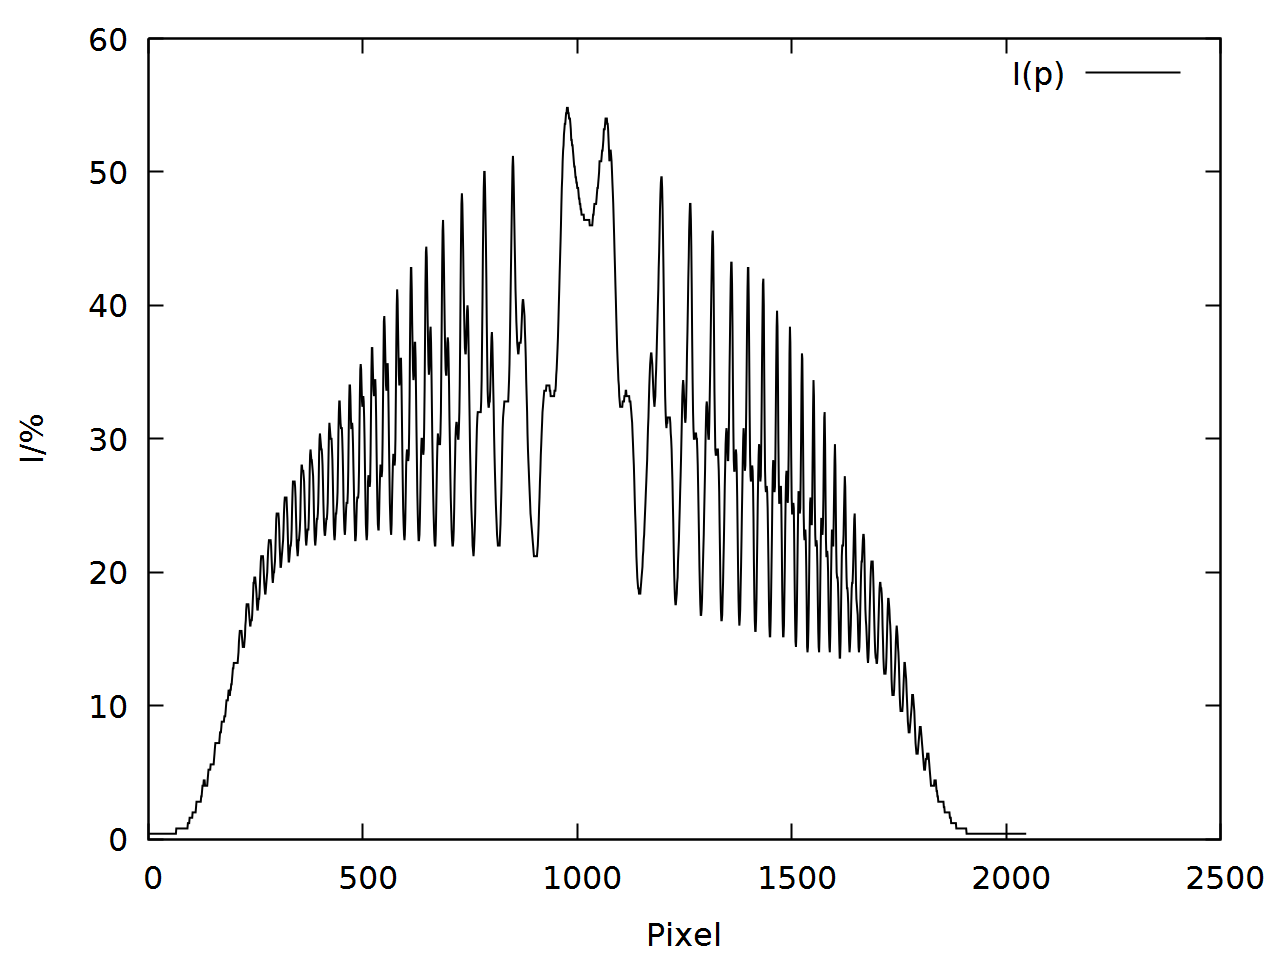
\includegraphics[width=\textwidth]{data/zeeman/out_6_0_raw.png}
\subcaption{Messung mit $I = \si{6\ampere}$}
\end{subfigure}
\begin{subfigure}{0.45\textwidth}
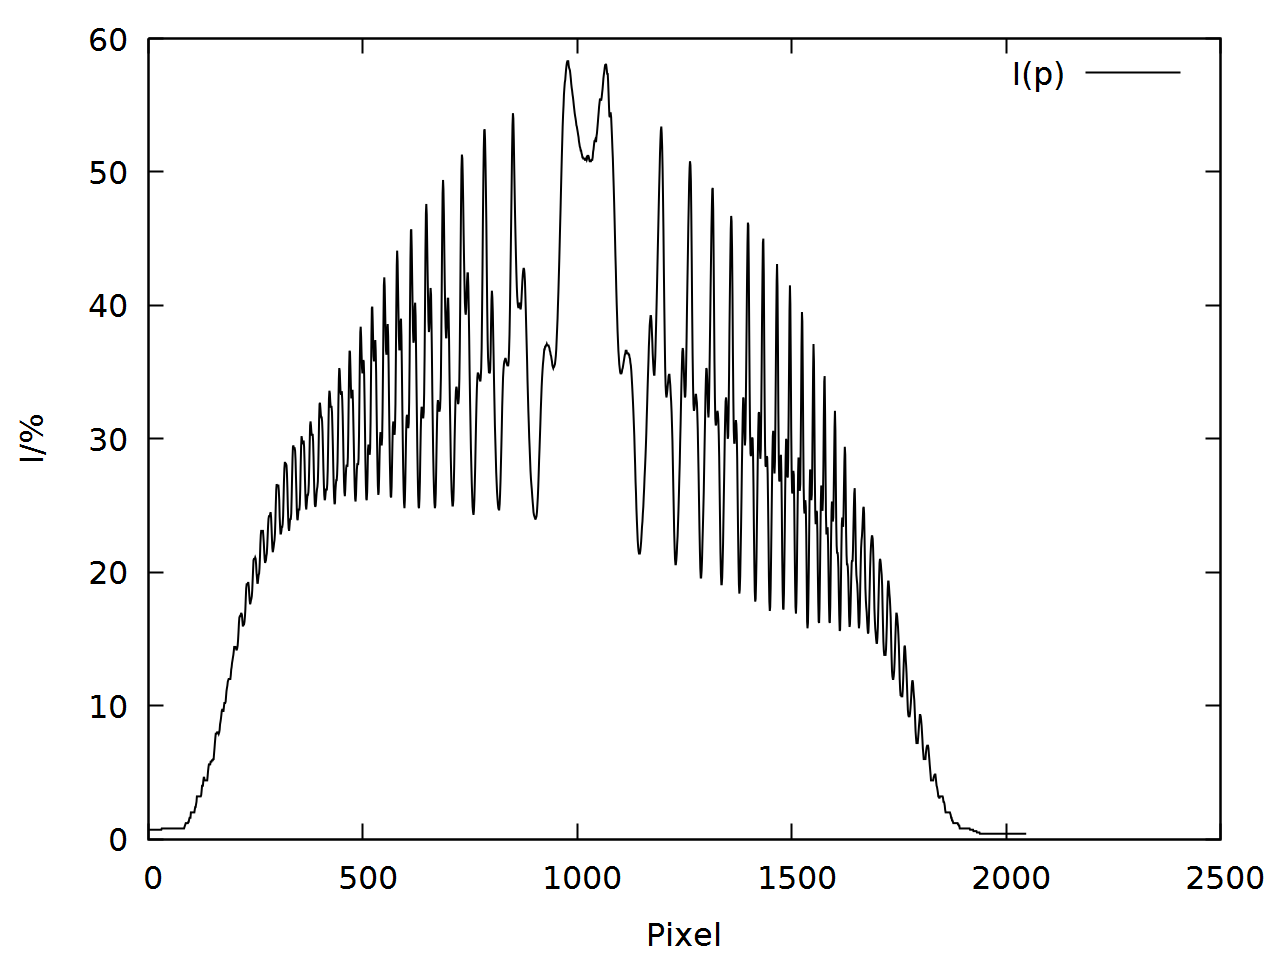
\includegraphics[width=\textwidth]{data/zeeman/out_6_3_raw.png}
\subcaption{Messung mit $I = \si{6,3\ampere}$}
\end{subfigure}
\begin{subfigure}{0.45\textwidth}
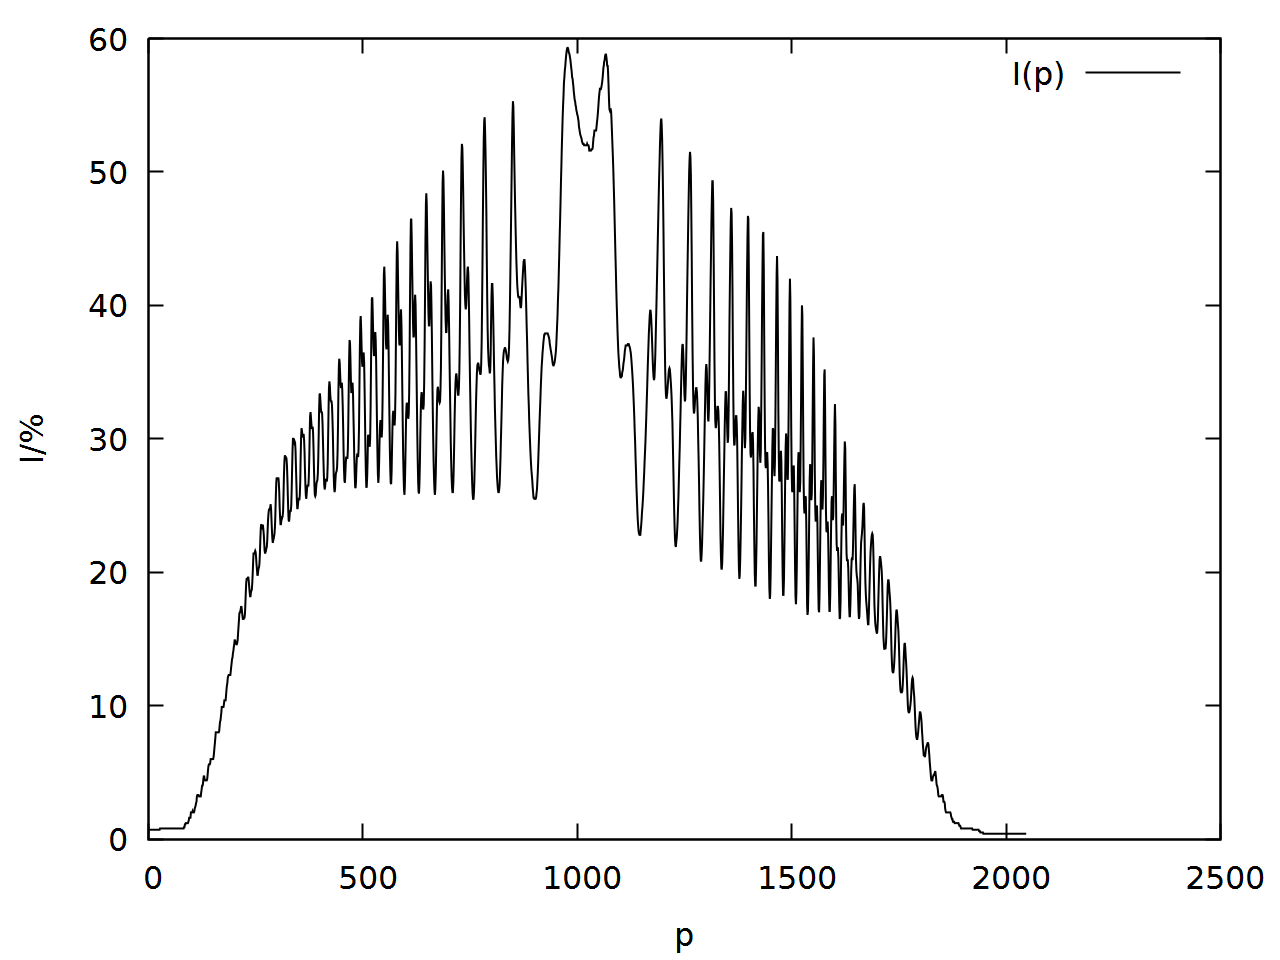
\includegraphics[width=\textwidth]{data/zeeman/out_6_6_raw.png}
\subcaption{Messung mit $I = \si{6,6\ampere}$}
\end{subfigure}
\begin{subfigure}{0.45\textwidth}
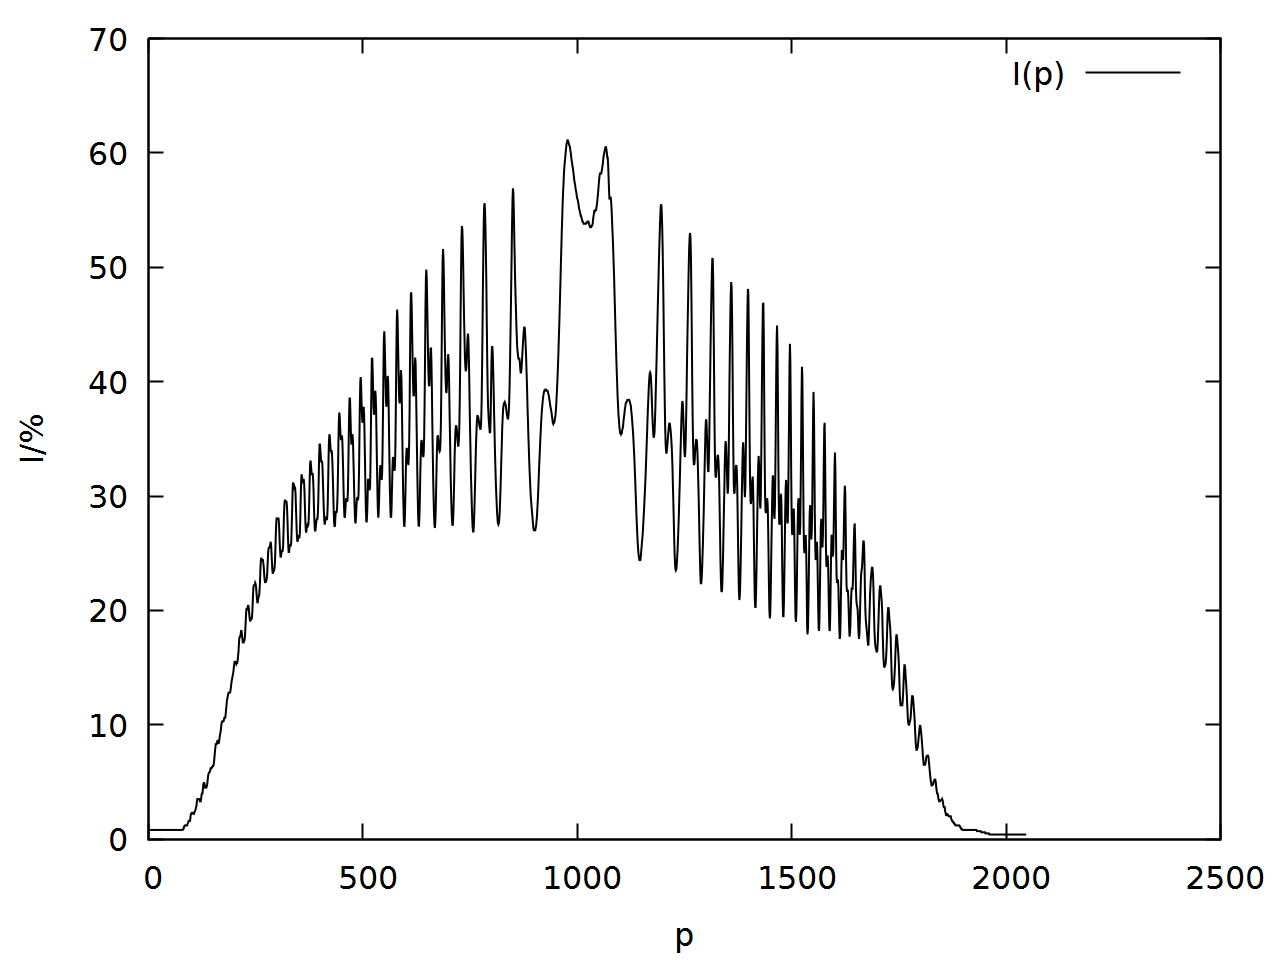
\includegraphics[width=\textwidth]{data/zeeman/out_6_9_raw.png}
\subcaption{Messung mit $I = \si{6,9\ampere}$}
\end{subfigure}
\begin{subfigure}{0.45\textwidth}
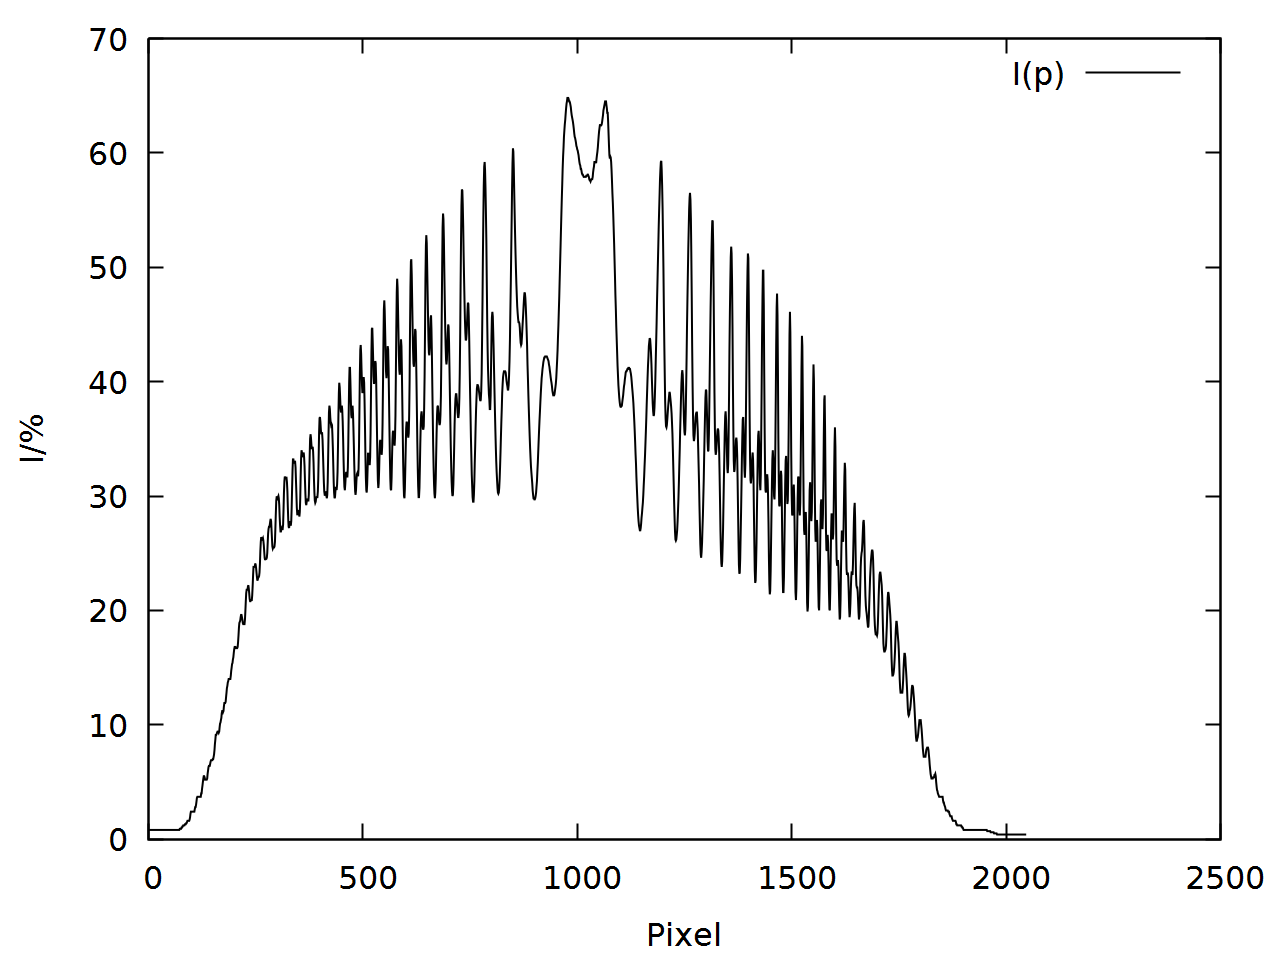
\includegraphics[width=\textwidth]{data/zeeman/out_7_2_raw.png}
\subcaption{Messung mit $I = \si{7,2\ampere}$}
\end{subfigure}
\begin{subfigure}{0.45\textwidth}
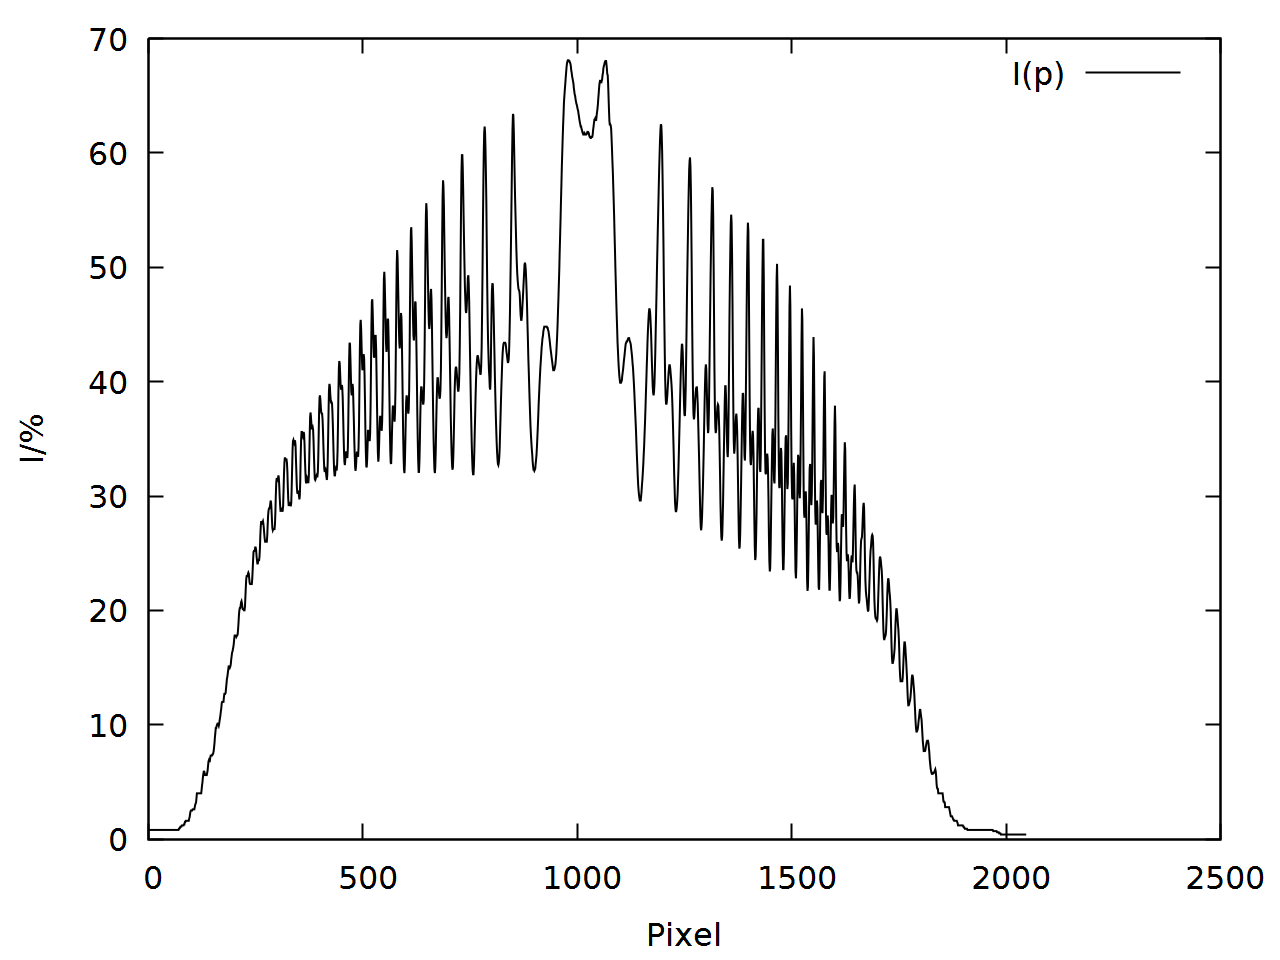
\includegraphics[width=\textwidth]{data/zeeman/out_7_5_raw.png}
\subcaption{Messung mit $I = \si{7,5\ampere}$}
\end{subfigure}
\caption{Messungen mit CCD-Kamera}
\label{fig:raw_1}
\end{figure}

\newpage

\begin{figure}
\centering
\begin{subfigure}{0.45\textwidth}
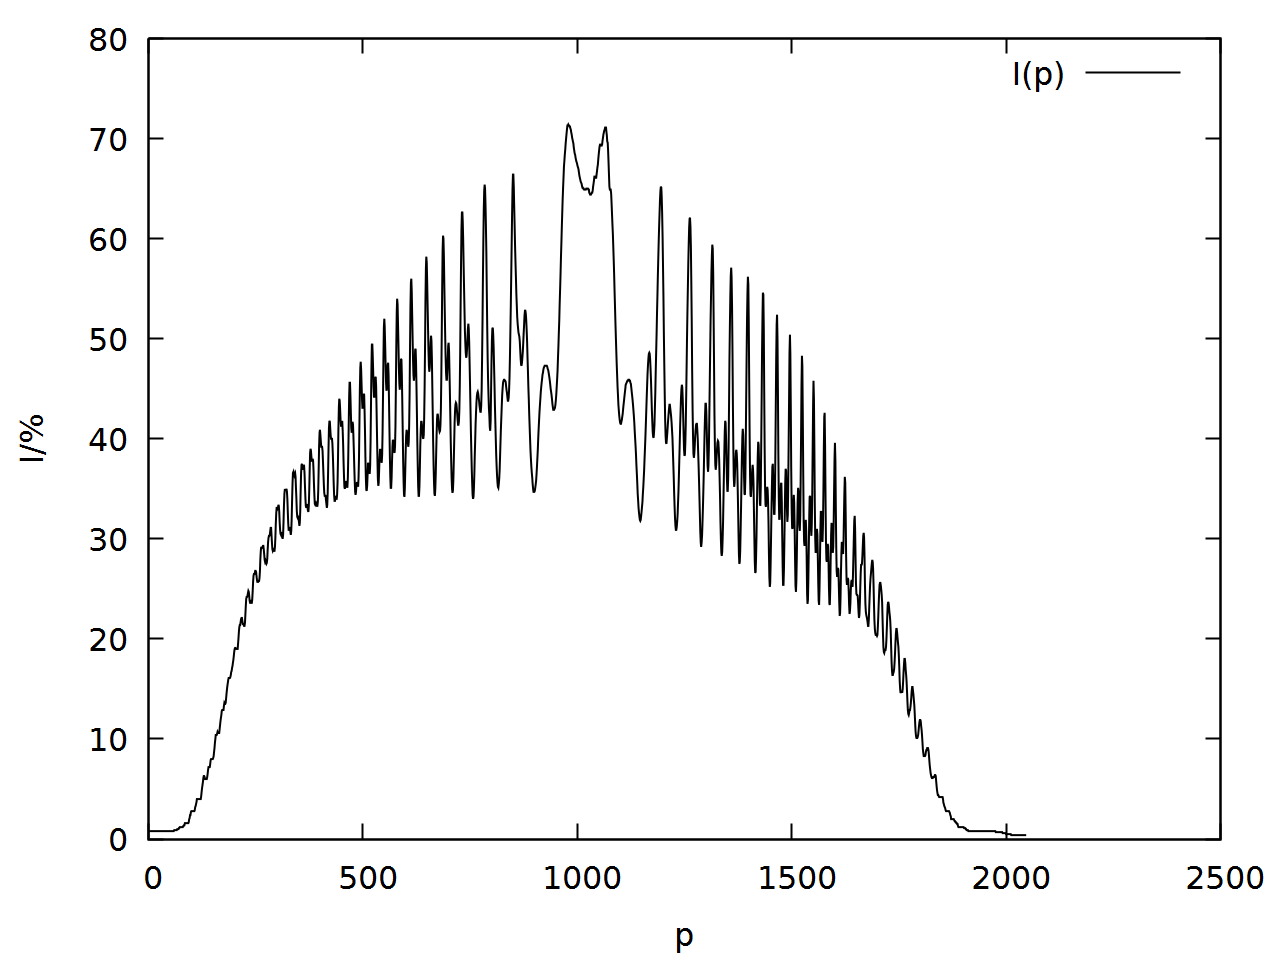
\includegraphics[width=\textwidth]{data/zeeman/out_7_8_raw.png}
\subcaption{Messung mit $I = \si{7,8\ampere}$}
\end{subfigure}
\begin{subfigure}{0.45\textwidth}
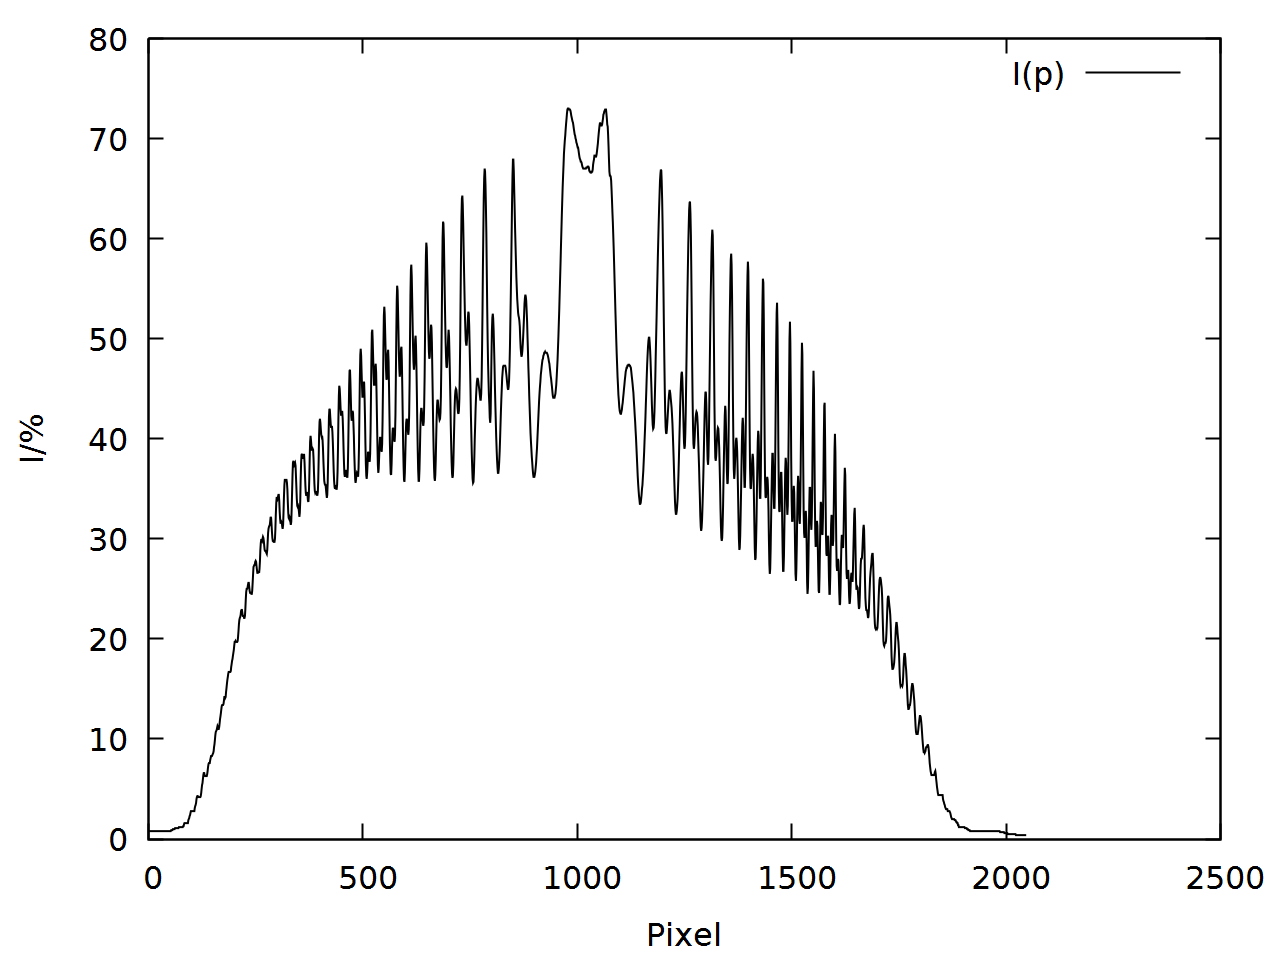
\includegraphics[width=\textwidth]{data/zeeman/out_8_1_raw.png}
\subcaption{Messung mit $I = \si{8,1\ampere}$}
\end{subfigure}
\begin{subfigure}{0.45\textwidth}
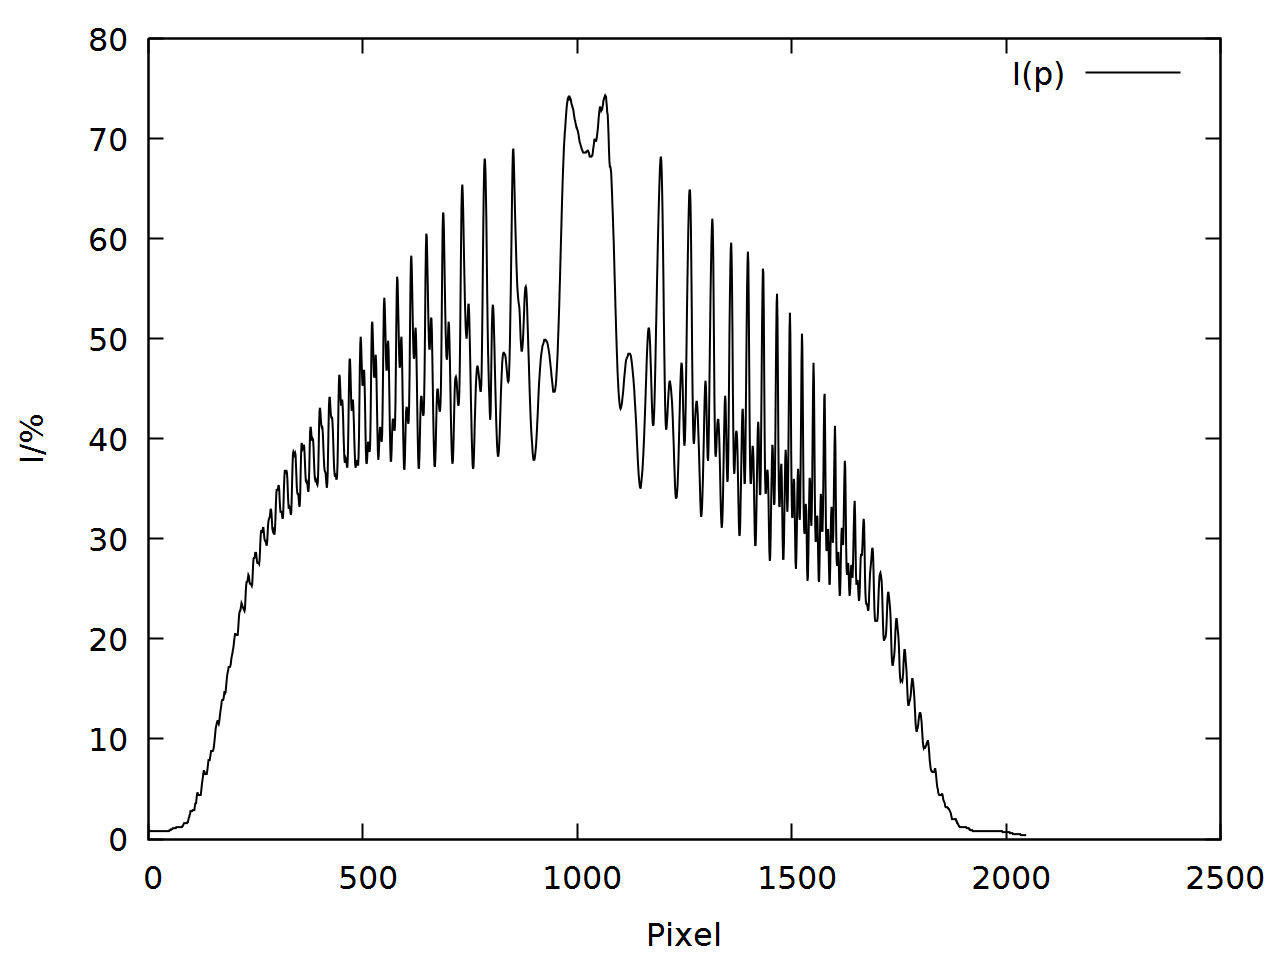
\includegraphics[width=\textwidth]{data/zeeman/out_8_4_raw.png}
\subcaption{Messung mit $I = \si{8,4\ampere}$}
\end{subfigure}
\begin{subfigure}{0.45\textwidth}
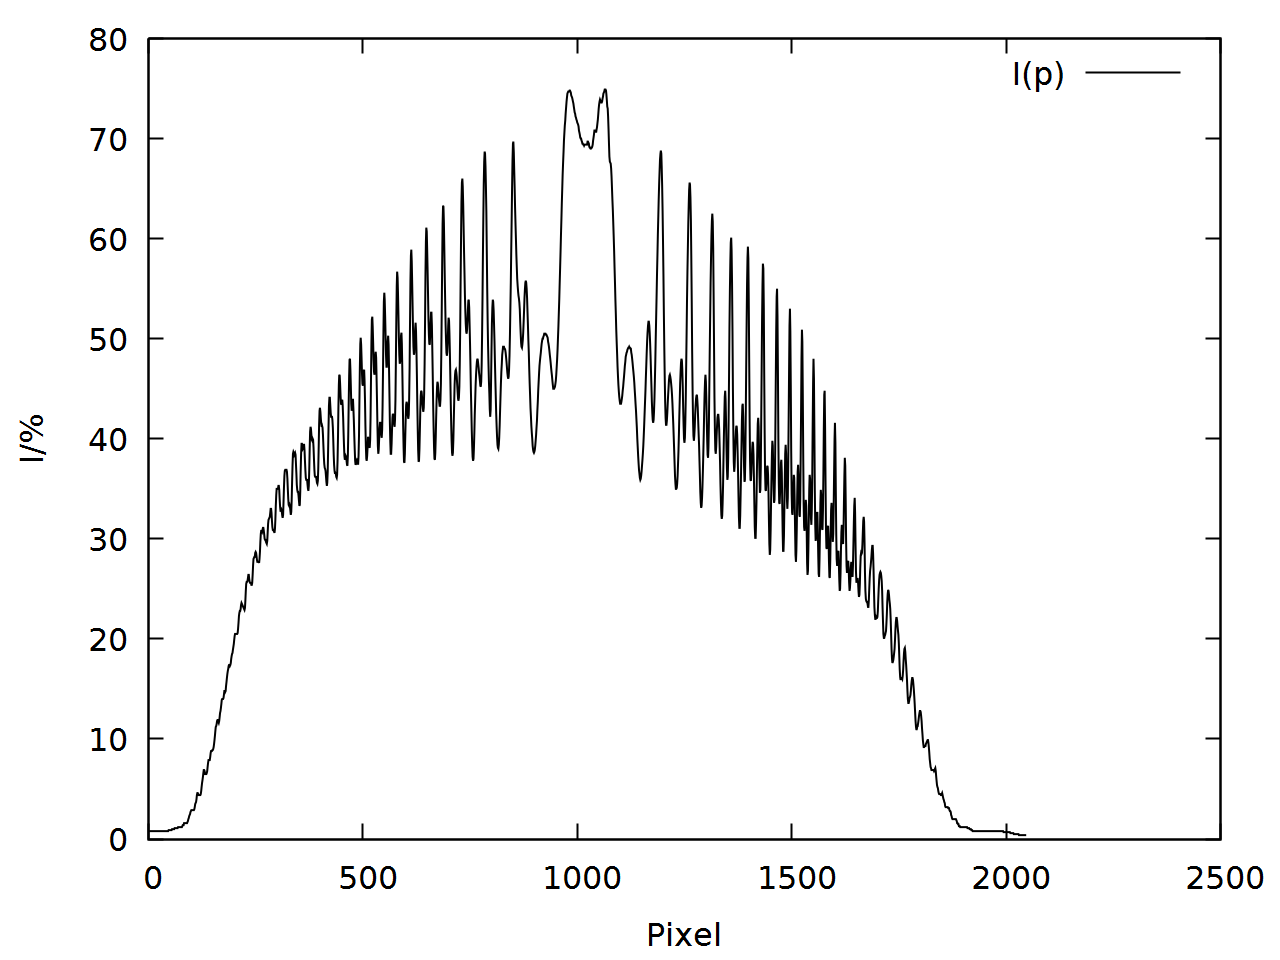
\includegraphics[width=\textwidth]{data/zeeman/out_8_5_raw.png}
\subcaption{Messung mit $I = \si{8,5\ampere}$}
\end{subfigure}
\caption{Weitere Messungen mit der CCD-Kamera}
\label{fig:raw}
\end{figure}

\paragraph{Bestimmung der Peaks}
Leider hat sich das mittlere Maximum nicht weit genug aufgespalten, so dass man die innere Linie auch sehen konnte. Wir verwenden deswegen zur Auswertung den zweitinnersten Ring. Wir betrachten demzufolge nur den Auschnitt, in dem sich die innersten beiden Ringe befinden. In dem Ausschnitt befinden sich also 10 Peaks (siehe Abb. \ref{fig:raw_fit}). An diese Peaks werden nur 10 überlagerte Gaussfunktionen gefittet ($I(p) = a\cdot \exp\left(-\frac{(p-b)^2}{2\cdot s^2}\right)$).


\begin{figure}
\centering
\begin{subfigure}{0.45\textwidth}
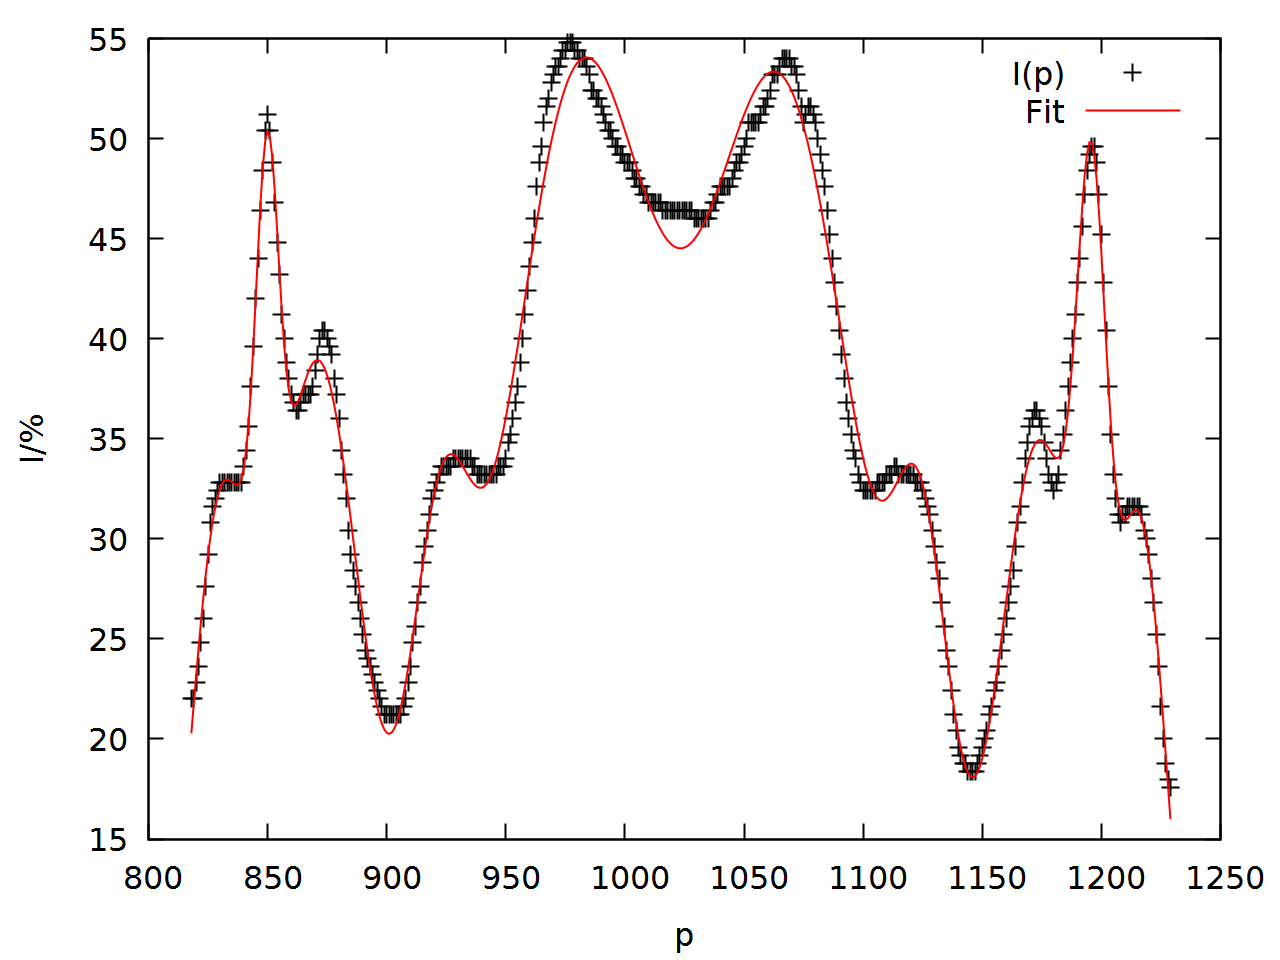
\includegraphics[width=\textwidth]{data/zeeman/out_6_0.png}
\subcaption{Messung mit $I = \si{6\ampere}$}
\end{subfigure}
\begin{subfigure}{0.45\textwidth}
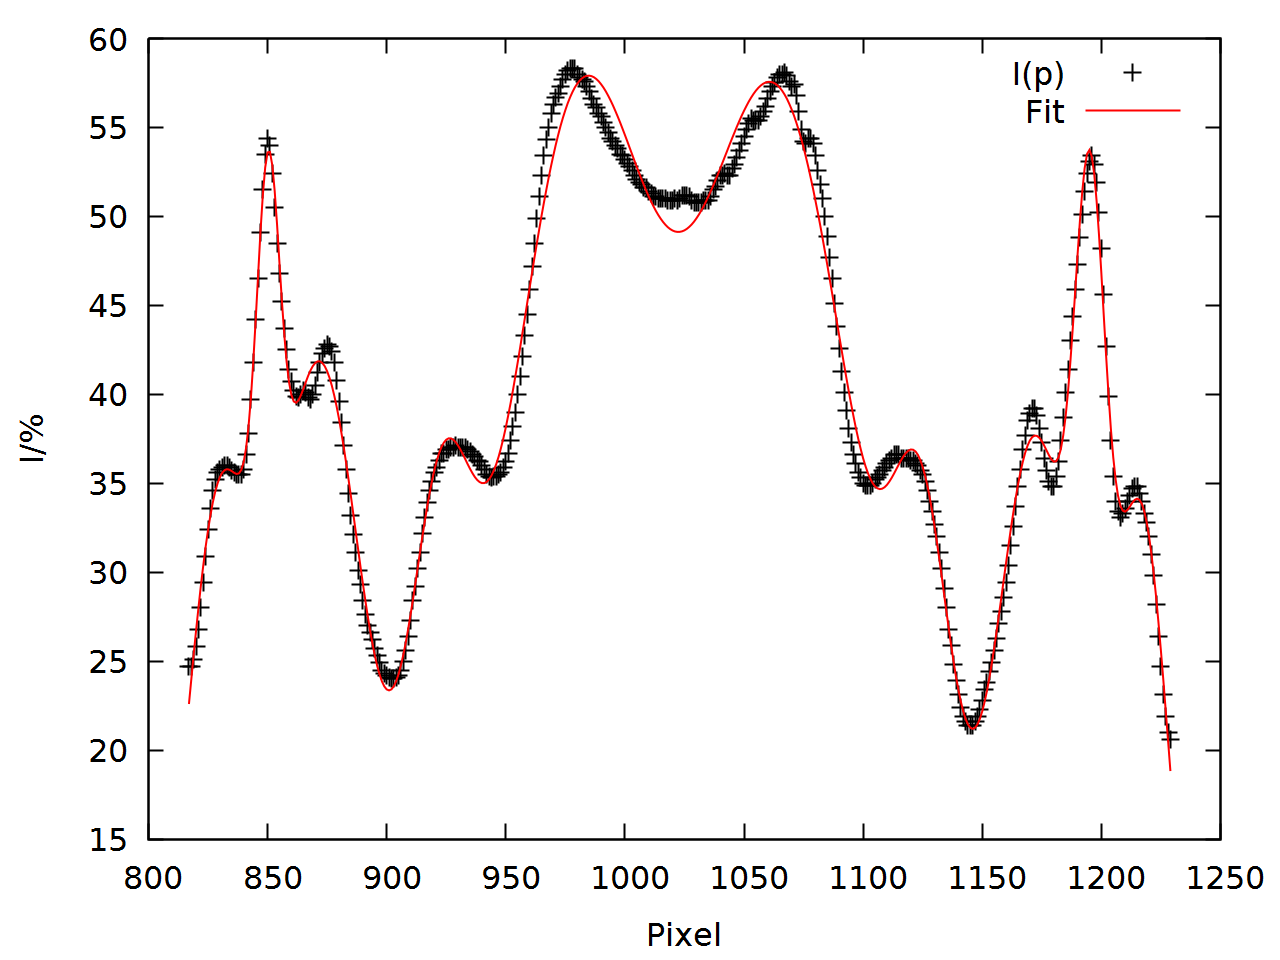
\includegraphics[width=\textwidth]{data/zeeman/out_6_3.png}
\subcaption{Messung mit $I = \si{6,3\ampere}$}
\end{subfigure}
\begin{subfigure}{0.45\textwidth}
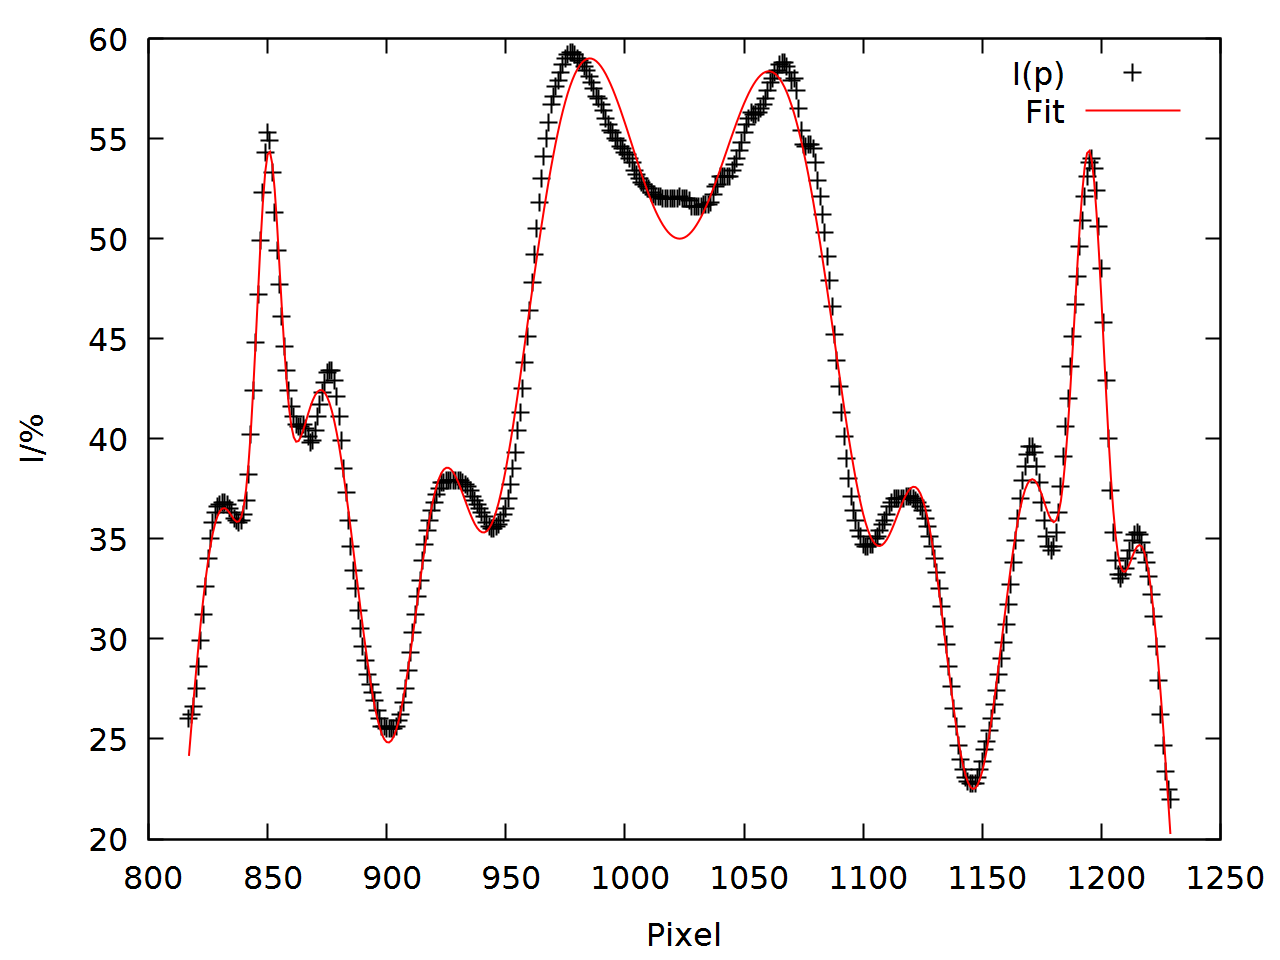
\includegraphics[width=\textwidth]{data/zeeman/out_6_6.png}
\subcaption{Messung mit $I = \si{6,6\ampere}$}
\end{subfigure}
\begin{subfigure}{0.45\textwidth}
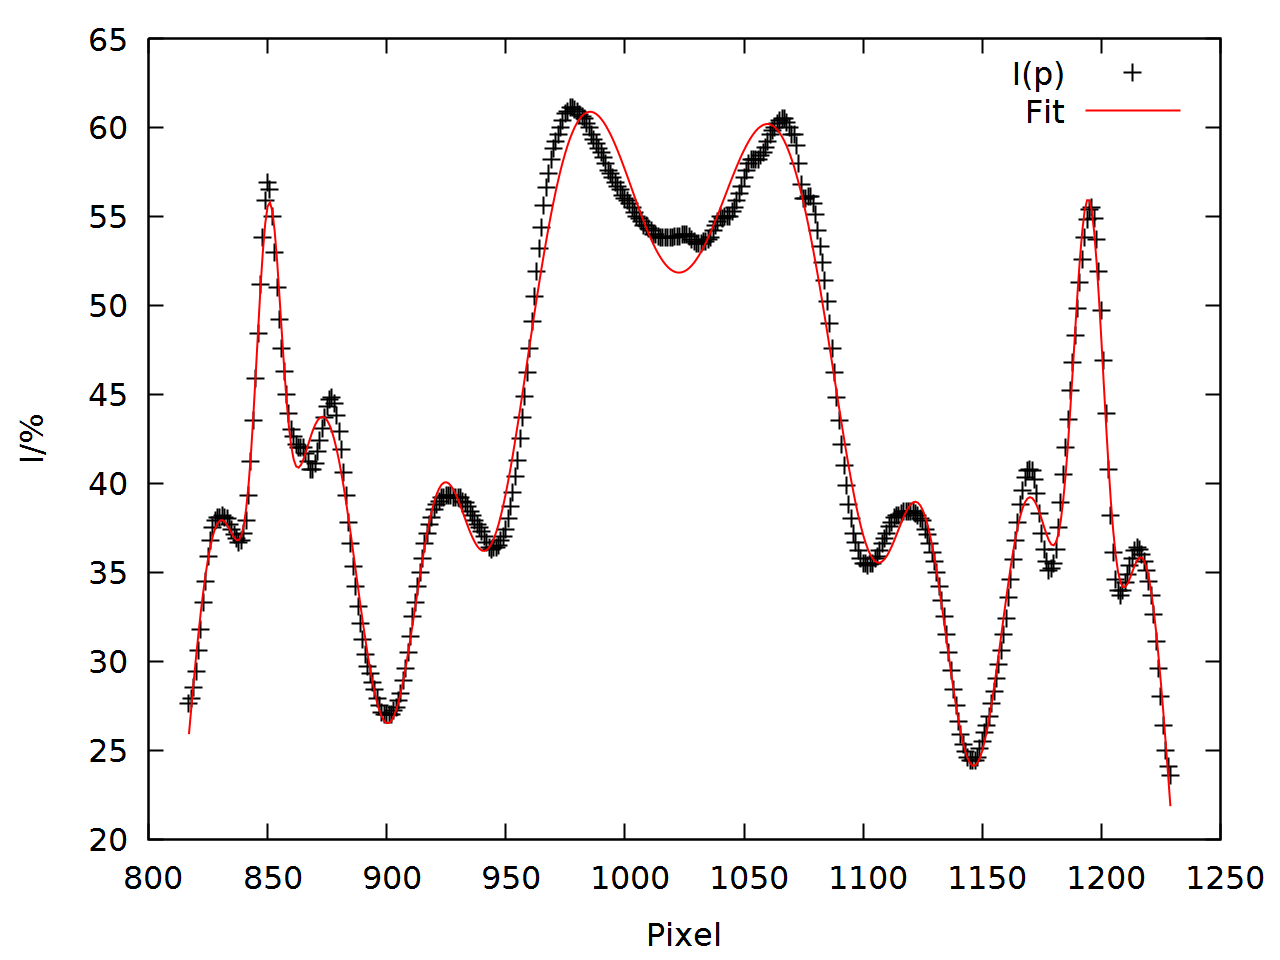
\includegraphics[width=\textwidth]{data/zeeman/out_6_9.png}
\subcaption{Messung mit $I = \si{6,9\ampere}$}
\end{subfigure}
\begin{subfigure}{0.45\textwidth}
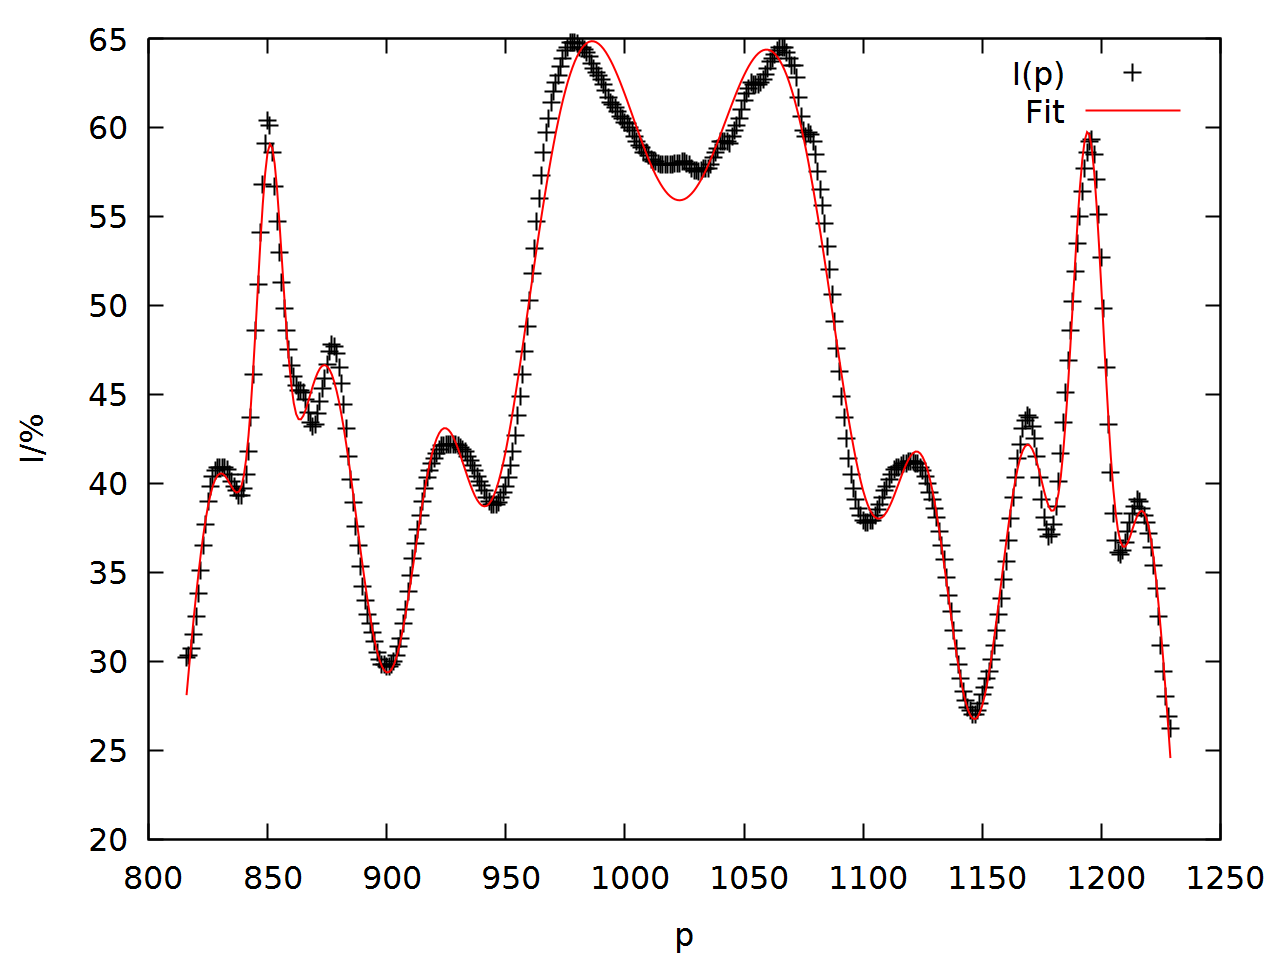
\includegraphics[width=\textwidth]{data/zeeman/out_7_2.png}
\subcaption{Messung mit $I = \si{7,2\ampere}$}
\end{subfigure}
\begin{subfigure}{0.45\textwidth}
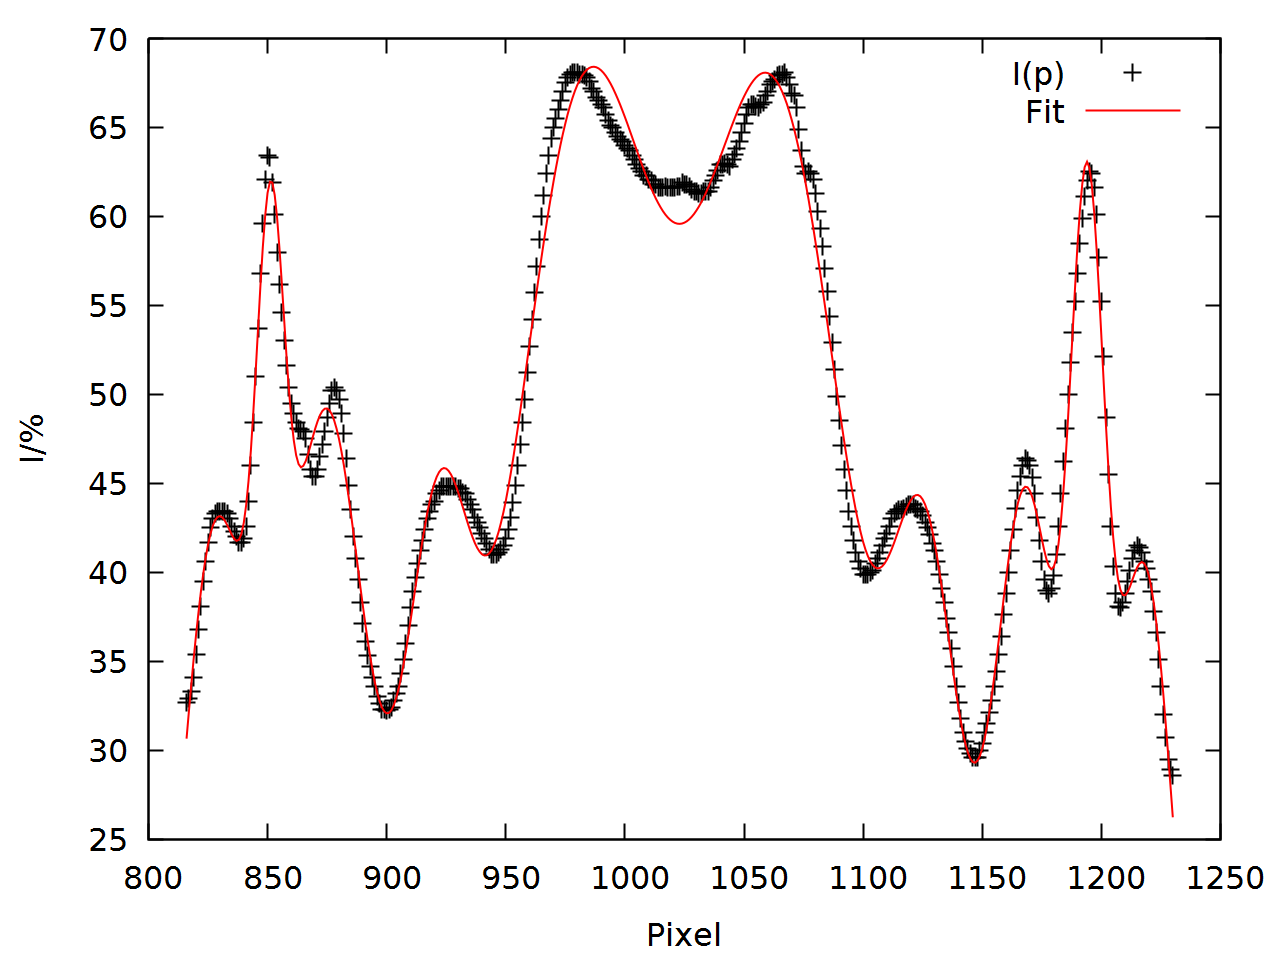
\includegraphics[width=\textwidth]{data/zeeman/out_7_5.png}
\subcaption{Messung mit $I = \si{7,5\ampere}$}
\end{subfigure}
\begin{subfigure}{0.45\textwidth}
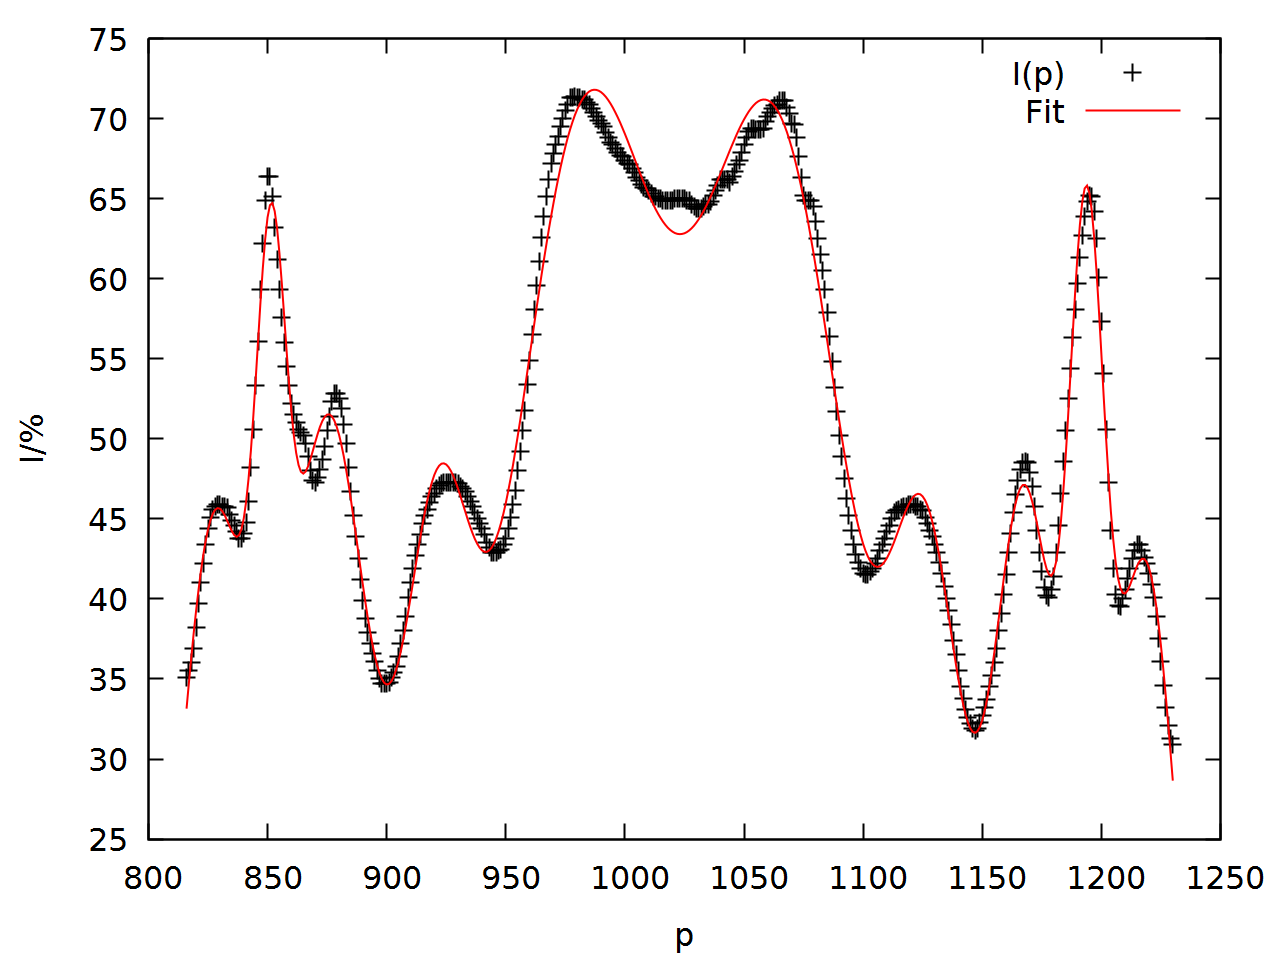
\includegraphics[width=\textwidth]{data/zeeman/out_7_8.png}
\subcaption{Messung mit $I = \si{7,8\ampere}$}
\end{subfigure}
\begin{subfigure}{0.45\textwidth}
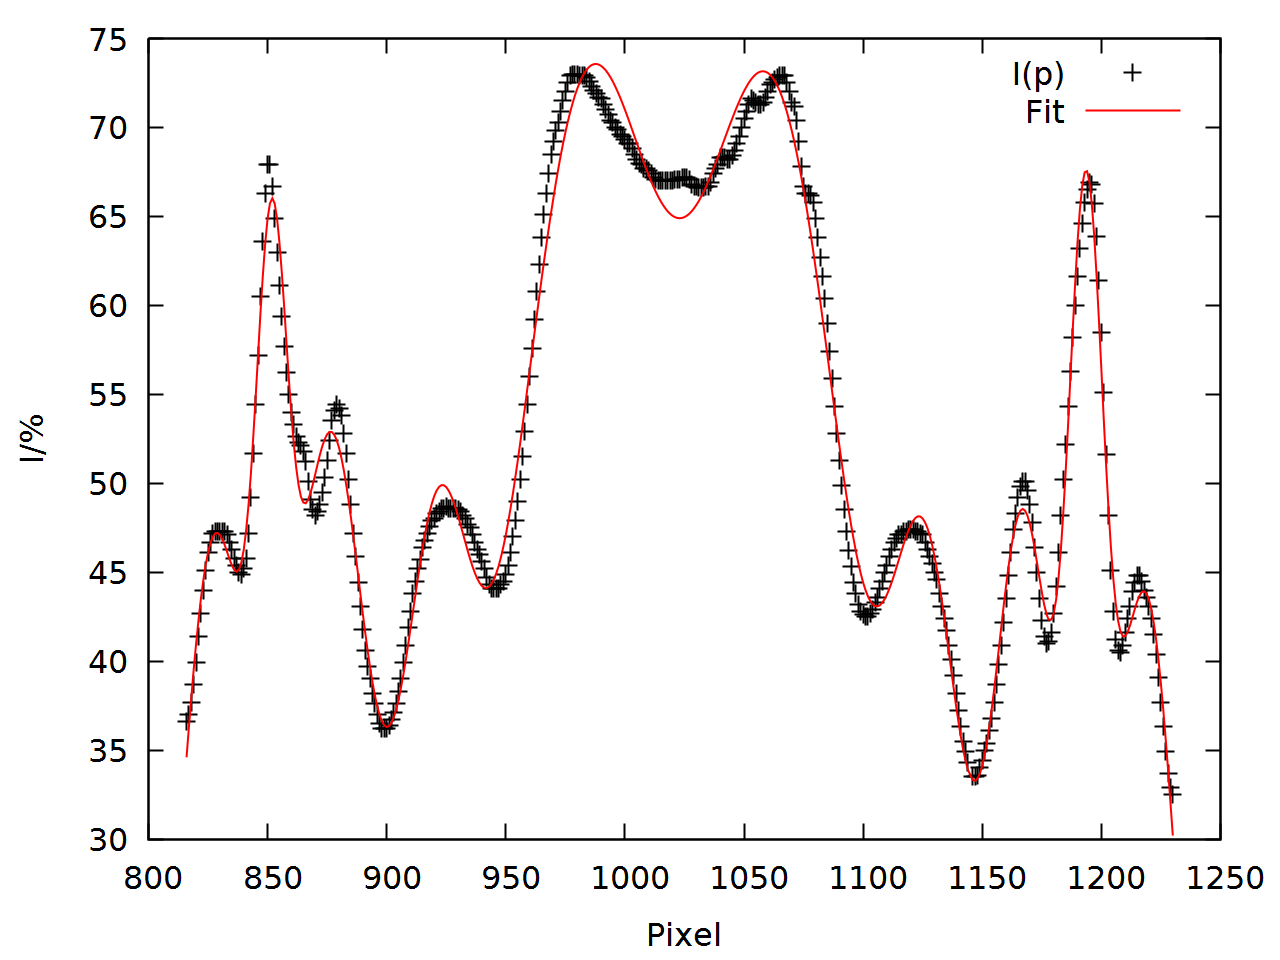
\includegraphics[width=\textwidth]{data/zeeman/out_8_1.png}
\subcaption{Messung mit $I = \si{8,1\ampere}$}
\end{subfigure}
\end{figure}
\begin{figure}\ContinuedFloat
\begin{subfigure}{0.45\textwidth}
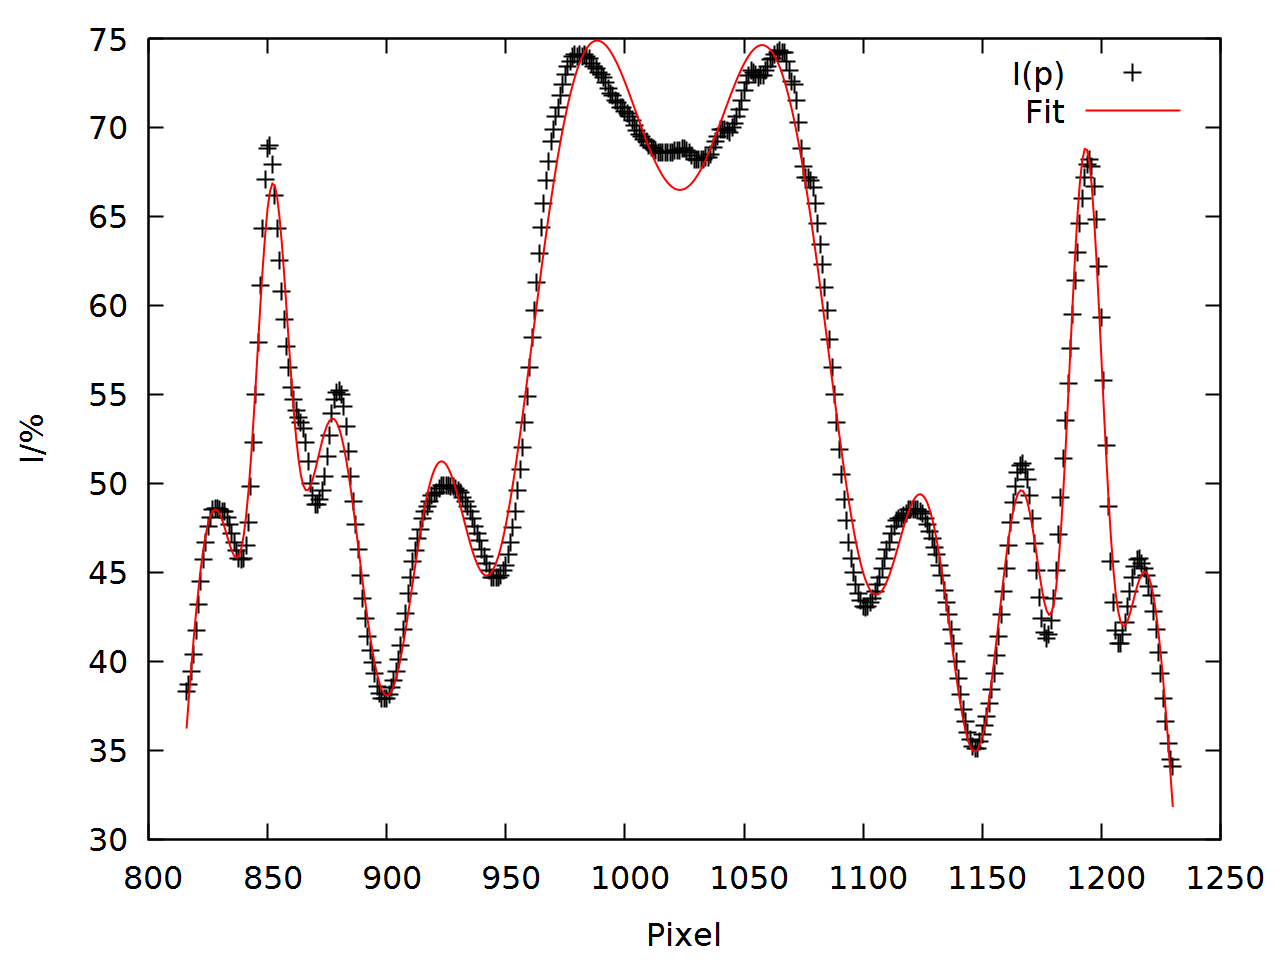
\includegraphics[width=\textwidth]{data/zeeman/out_8_4.png}
\subcaption{Messung mit $I = \si{8,4\ampere}$}
\end{subfigure}
\begin{subfigure}{0.45\textwidth}
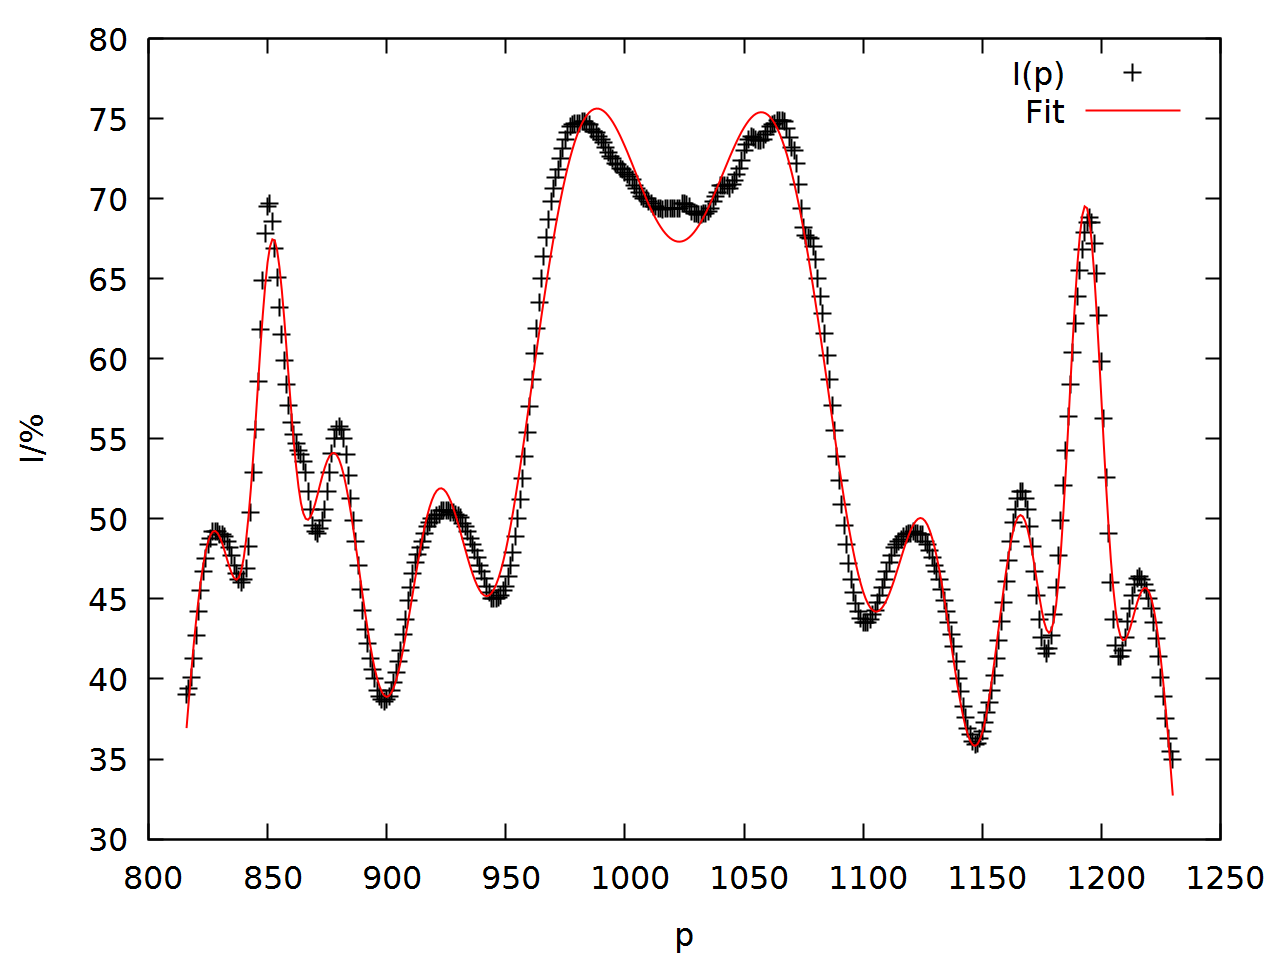
\includegraphics[width=\textwidth]{data/zeeman/out_8_5.png}
\subcaption{Messung mit $I = \si{8,5\ampere}$}
\end{subfigure}
\caption{Fits an die Messungen}
\label{fig:raw_fit}
\end{figure}

Die Ergebnisse der Fits sind in Tab. \ref{tab:werte} im Anhang aufgelistet (Die Nummern $n$ stehen für die Reihenfolge der Peaks von links nach rechts). Aus den $b$-Werten kann man den Winkel der Peaks über die Relation aus \cite{praktikumsheft} ermitteln:
\begin{align*}
\alpha &= \tan^{-1}\left(\frac{(1024-b)\cdot 0,014\si{\milli\meter}}{150\si{\milli\meter}}\right) & \frac{(1024-b)\cdot 0,014\si{\milli\meter}}{150\si{\milli\meter}} \ll 1\\
&\approx \frac{(1024-b)\cdot 0,014\si{\milli\meter}}{150\si{\milli\meter}}\\
\Delta \alpha &= \frac{\Delta b\cdot 0,014\si{\milli\meter}}{150\si{\milli\meter}}
\end{align*}   
Daraus ergibt sich der Gangunterschied zweier Strahlen (Etalon: $d = 4\si{\milli\meter}, n = 1,457, r = 0,85$, Farbfilter: $\lambda = (643,8\pm 2,0) \si{\nano\meter}$):
\begin{align*}
g &= 2\cdot d \cdot \sqrt{n^2 - \sin^2{\alpha}} \approx 2\cdot d \cdot \sqrt{n^2 - \alpha^2}\\
\Delta g &= 2\cdot d \frac{\alpha \Delta\alpha}{\sqrt{n^2 - \alpha^2}}
\end{align*}
Diese Werte sind auch in Tab. \ref{tab:werte} eingetragen. Die Wellenlänge könnte nun theoretisch berechnet werden, indem man diesen Gangunterschied durch die Ordnung des Maximums $m$ teilt. Diese ist allerdings nicht bekannt und kann nur mit großen Fehler aus der Dicke des Etalons berechnet werden. Da wir aber nur die Energieverschiebung berechnen sollen, ist die Ordnung des Maximums nicht relevant:
\begin{align*}
\delta E &\approx -\frac{hc}{\lambda_\pi^0} \frac{\lambda_{\sigma^\pm} - \lambda_\pi}{\lambda_{\sigma^\pm}}\\
	&= -\frac{hc}{\lambda_\pi^0} \frac{m \lambda_{\sigma^\pm} - m \lambda_\pi}{m\lambda_{\sigma^\pm}}\\
	& = -\frac{hc}{\lambda_\pi^0} \frac{g_{\sigma^\pm} - g_\pi}{g_{\sigma^\pm}}\\
\Delta \delta E &= \delta E \sqrt{\left(\frac{\sqrt{\Delta g_{\sigma^\pm}^2 + \Delta g_\pi^2}}{g_{\sigma^\pm} - g_\pi}\right)^2 + \left(\frac{\Delta g_{\sigma^\pm}}{g_{\sigma^\pm}}\right)^2}
\end{align*}

Diese Energieverschiebungen werden nun für alle 6 $\sigma$-Peaks relativ zu ihrem $\pi$-Peak berechnet. Der Betrag der Ergebnisse wird über dem berechnetem Magnetfeld aufgetragen (siehe Abb. \ref{fig:res_lin} und Abb. \ref{fig:res_prop}). An diesen Daten führen wir zwei lineare Fits durch, einmal mit $\delta E = a_1 B + b_1$ (siehe Abb. \ref{fig:res_lin}) und einmal ohne Achsenabschnitt $\delta E = a_2 B$ (siehe Abb. \ref{fig:res_prop}). Die Ergebnisse sind in Tab. \ref{tab:res} aufgelistet.\\
\begin{figure}
\centering
\begin{subfigure}{0.6\textwidth}
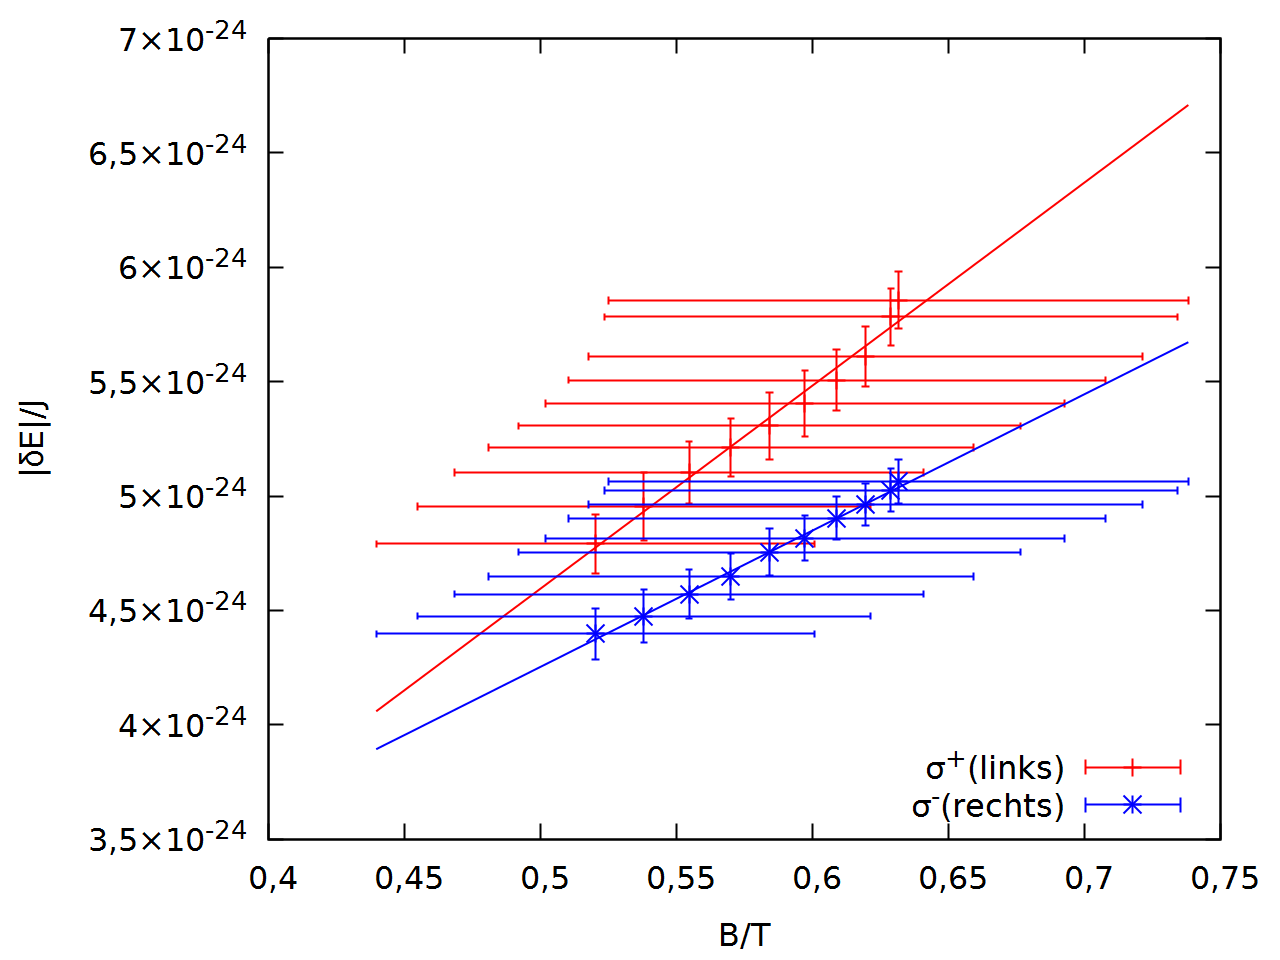
\includegraphics[width=\textwidth]{data/zeeman/out_zeeman_neu_links.png}
\subcaption{Linker Peak}
\end{subfigure}
\begin{subfigure}{0.6\textwidth}
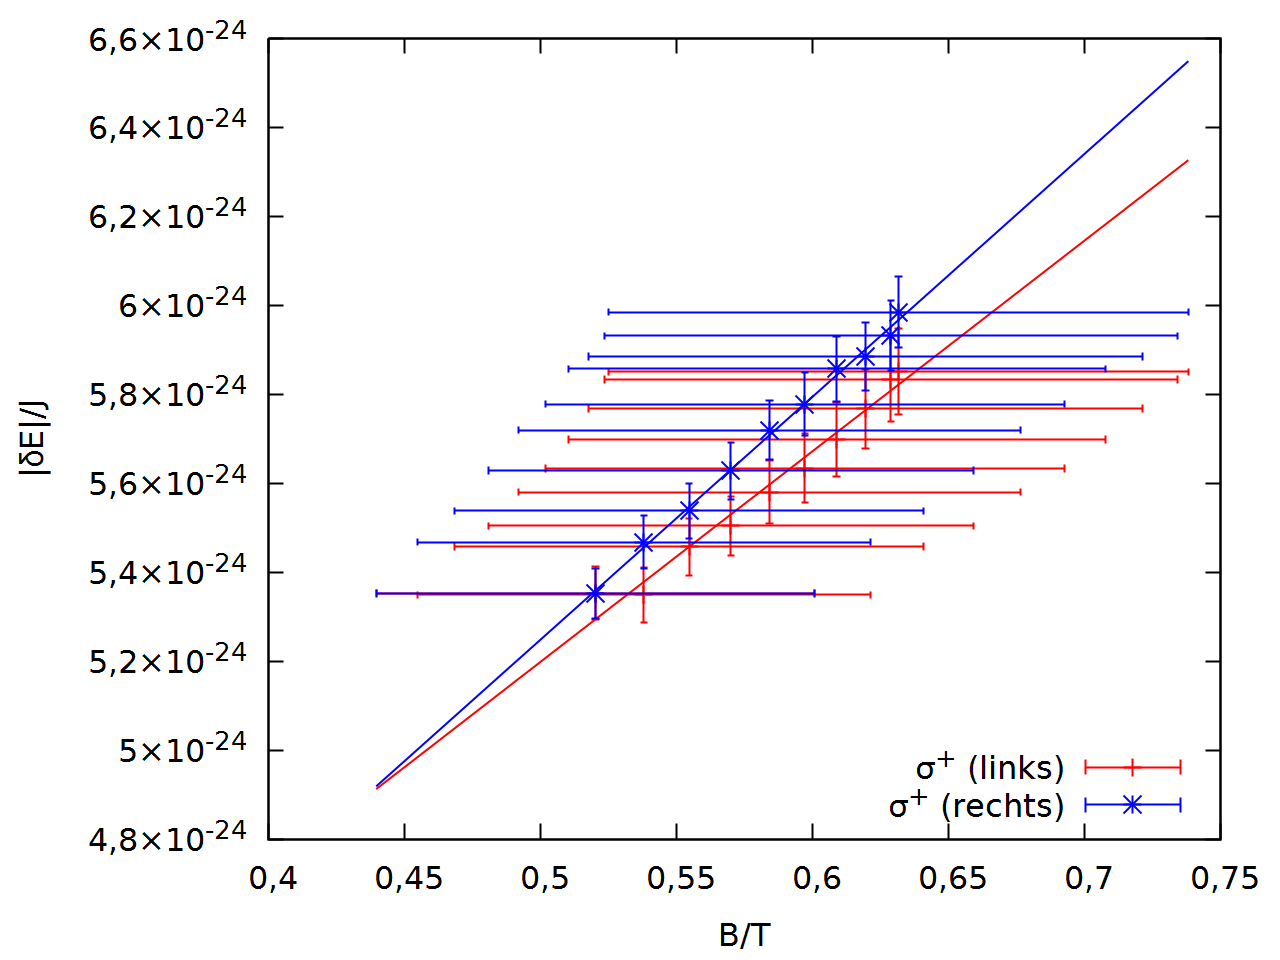
\includegraphics[width=\textwidth]{data/zeeman/out_zeeman_neu_mitte.png}
\subcaption{Mittige Peaks}
\end{subfigure}
\begin{subfigure}{0.6\textwidth}
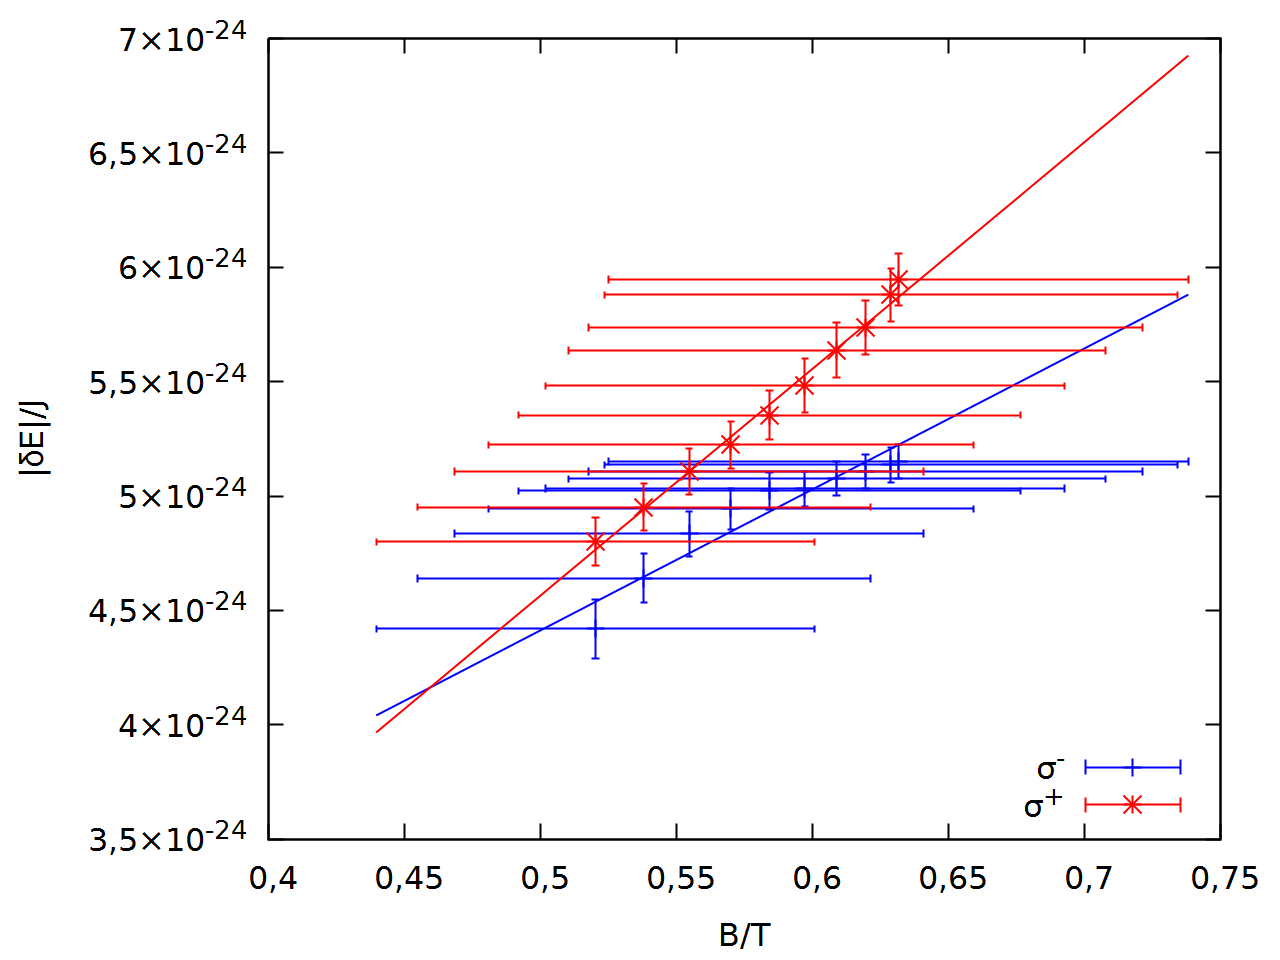
\includegraphics[width=\textwidth]{data/zeeman/out_zeeman_neu_rechts.png}
\subcaption{Rechter Peak}
\end{subfigure}
\caption{Energieverschiebung mit linearem Fit $\delta E = b_1 + B \cdot a_1$}
\label{fig:res_lin}
\end{figure}

\begin{figure}
\centering
\begin{subfigure}{0.6\textwidth}
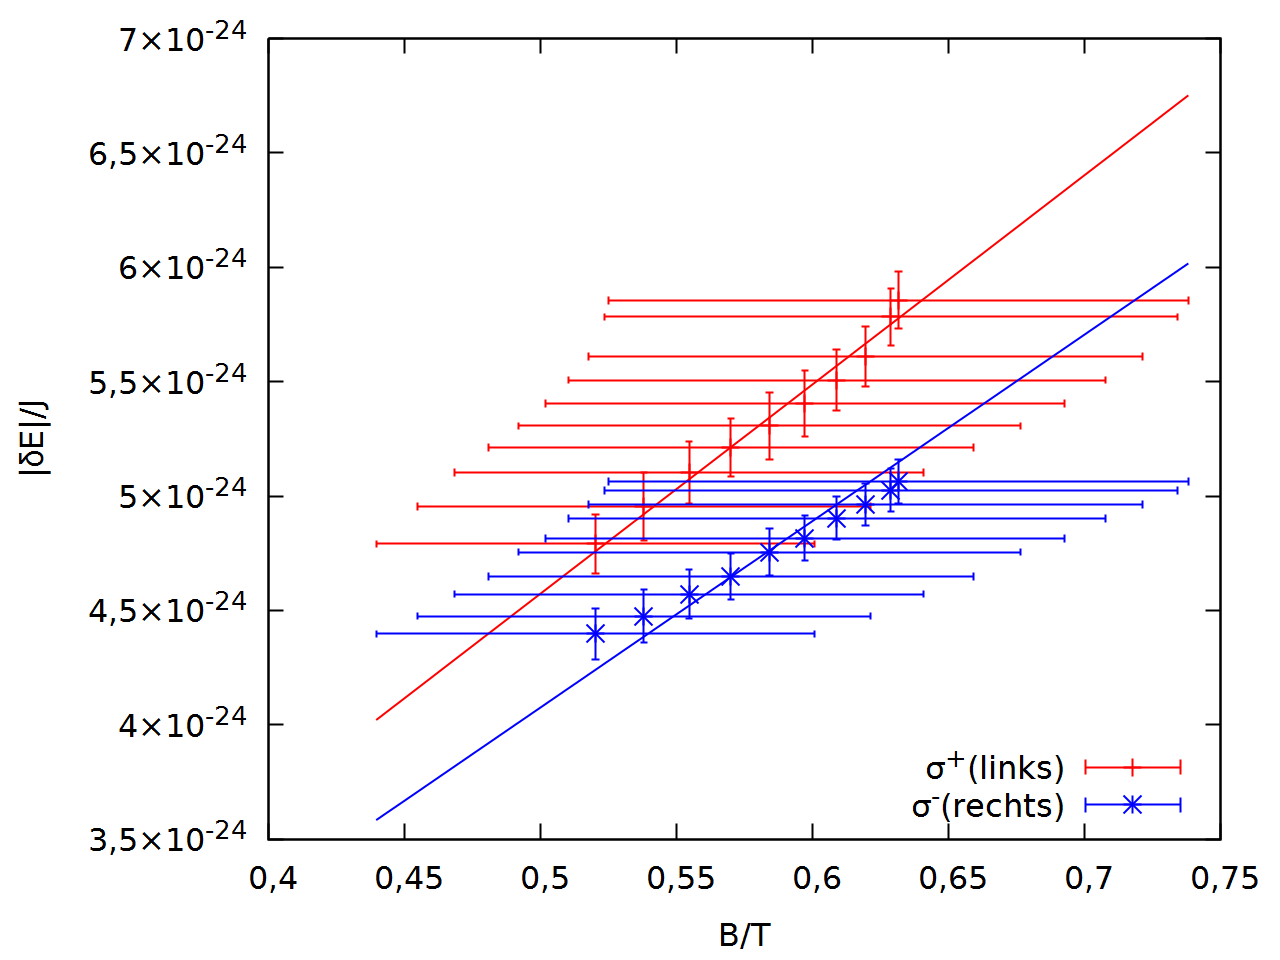
\includegraphics[width=\textwidth]{data/zeeman/out_zeeman_neu_links_prop.png}
\subcaption{Linker Peak}
\end{subfigure}
\begin{subfigure}{0.6\textwidth}
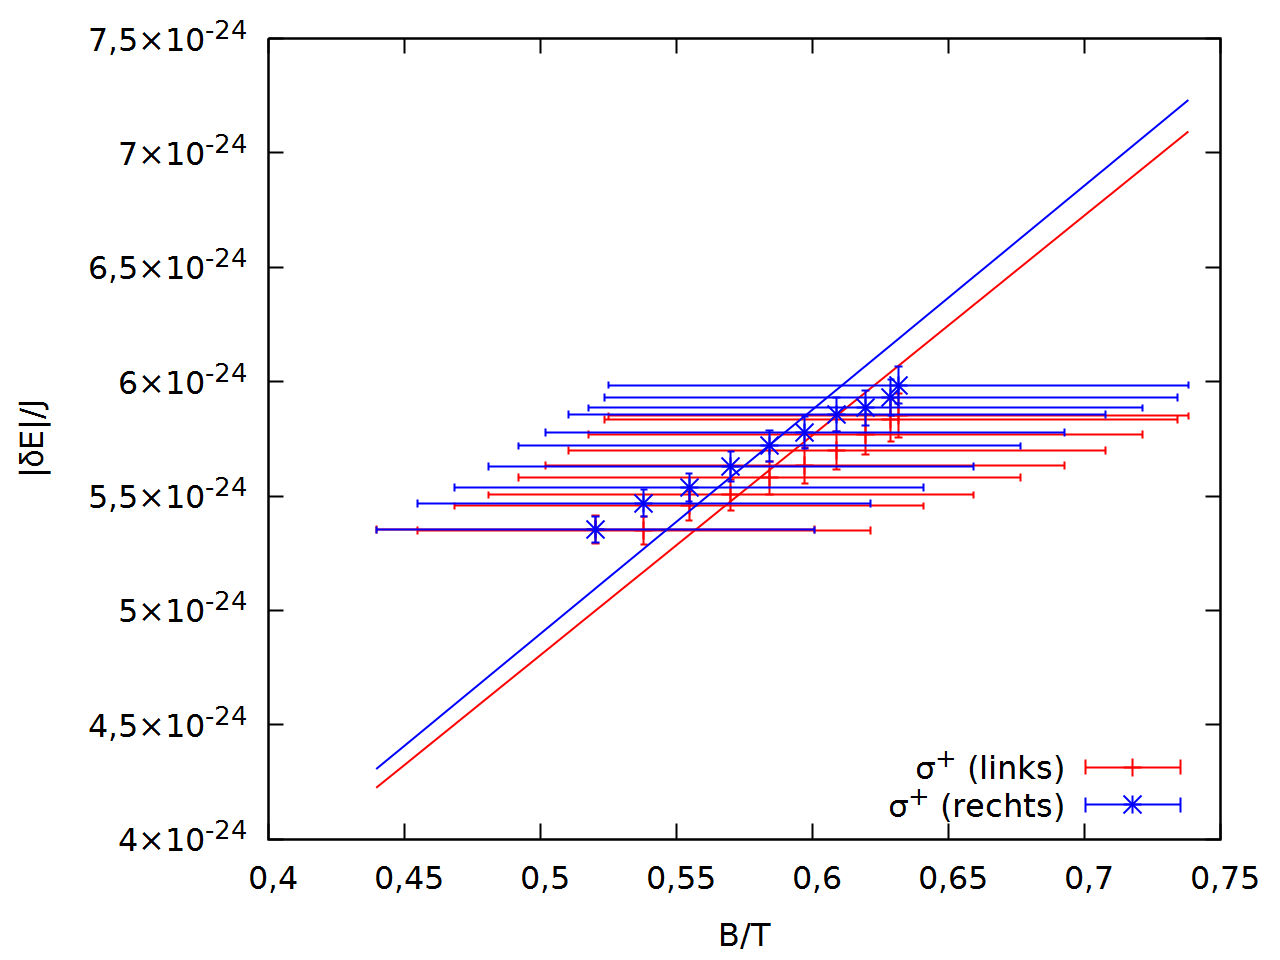
\includegraphics[width=\textwidth]{data/zeeman/out_zeeman_neu_mitte_prop.png}
\subcaption{Mittige Peaks}
\end{subfigure}
\begin{subfigure}{0.6\textwidth}
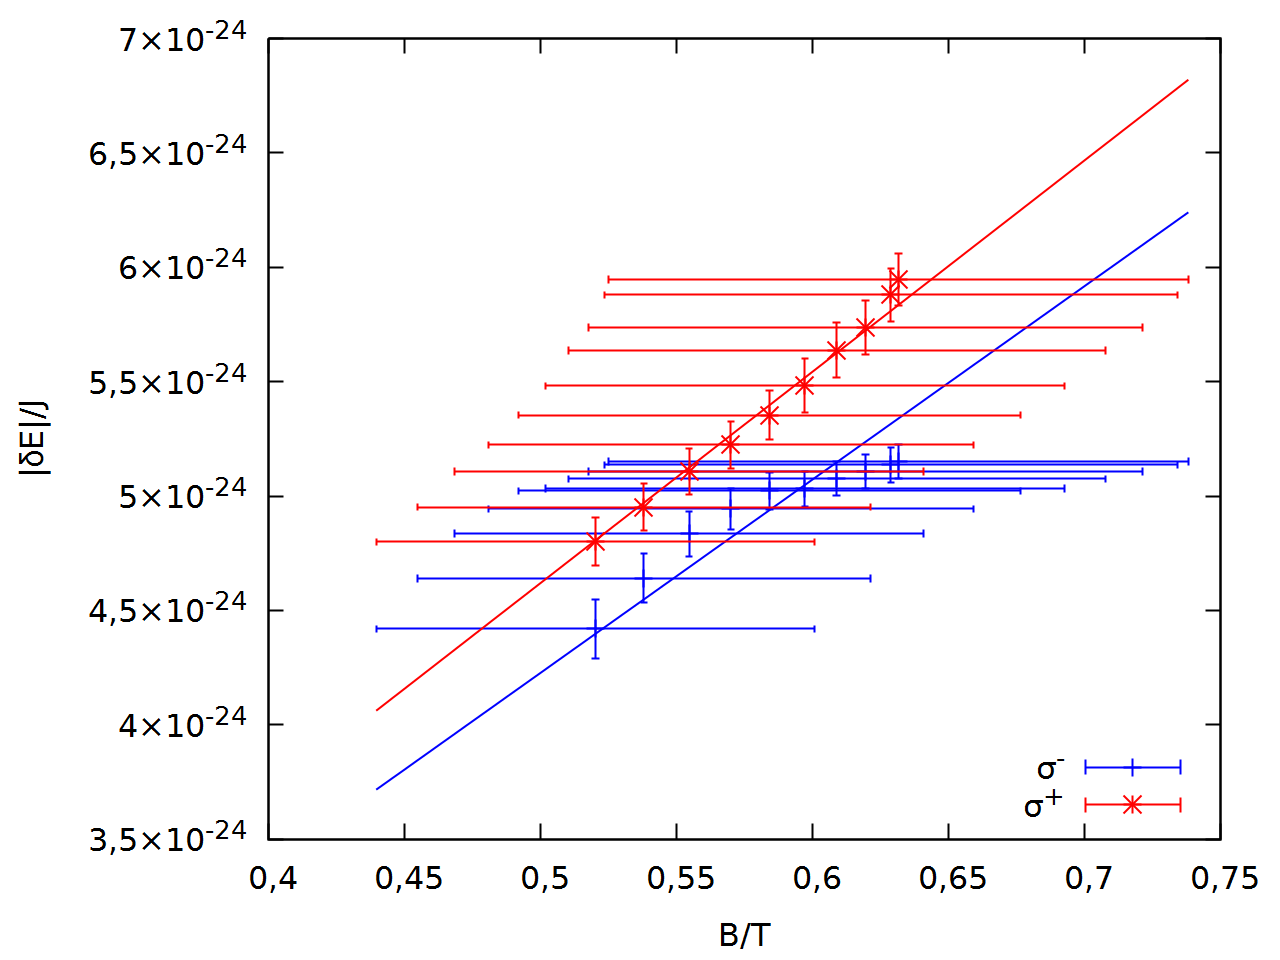
\includegraphics[width=\textwidth]{data/zeeman/out_zeeman_neu_rechts_prop.png}
\subcaption{Rechter Peak}
\end{subfigure}
\caption{Energieverschiebung mit Fit ohne Achsenabschnitt $\delta E = B \cdot a_2$}
\label{fig:res_prop}
\end{figure}

\begin{table}[h]
\centering
\caption{Ergebnisse der Fits}
\label{tab:res}
\begin{tabular}{l>{$}c<{$}>{$}c<{$}>{$}c<{$}}
\toprule
Peak & a_1/\si{10^{-24} \joule\tesla^{-1}} & b_1/\si{10^{-24} \joule} & a_2/\si{10^{-24} \joule\tesla^{-1}}\\
\midrule
links $\sigma^+$ (links) & 8,9 \pm 0,4 &  0,2 \pm 0,2& 9,15 \pm 0,026\\
links $\sigma^-$ (rechts) & 6,0 \pm 0,1 & 1,27 \pm 0,08& 8,15 \pm 0,05\\
mitte $\sigma^+$ (links) & 4,7 \pm 0,3 & 2,8 \pm  0,16& 9,6 \pm 0,1\\
mitte $\sigma^+$ (rechts) & 5,5 \pm 0,1 & 2,52 \pm 0,06& 9,80 \pm 0,09\\        
rechts $\sigma^-$ (links) & 6,2 \pm 0,7 & 1,3 \pm 0,4& 8,45 \pm 0,07\\
rechts $\sigma^+$ (rechts) & 9,9 \pm 0,3 & -0,4 \pm 0,2& 9,24 \pm 0,03\\ 
\bottomrule
\end{tabular}
\end{table}

\newpage

Man kann gut erkennen, dass sich die linearen Fits mit Achsenabschnitt deutlich besser an die Daten anpassen. Allerdings liegt ein proportionaler Zusammenhang auch im Fehlerbereich des Magnetfeldes. Der große Fehler des Magnetfeldes stammt von den zwei unterschiedlichen Kalibrierungskurven. Während der Messung ging der Zusammenhang von der einen Kurve über in den Zusammenhang der anderen Kurve. Je nach Ablauf dieses Übergangs wären die Diagramme in der x-Richtung gestreckt bzw. gestaucht. Würde man die Daten wieder etwas stauchen, so würden die Messpunkte auf einer steileren Gerade liegen und somit proportional zum Magnetfeld sein.\\
Weiterhin kann man erkennen, dass die beiden äußersten Peaks eine deutlich steilere Kurve aufweisen als die inneren. Das liegt an der Art der Bestimmung der Peaks. Das gesamte Interferenzbild ist eine Überlagerung von Gaussfunktionen. In der Mitte ist der Fit genauer, da man da auch die Überlagerung mit benachbarten Peaks mitbetrachtet. Bei den Peaks am Rand geschieht das nicht. Somit könnte hier ein systematischer Fehler aufgetreten sein.\\
 
Durch Mittelwertbildung der $a$-Werte (Fehler durch Standartabweichung) ergibt sich für das Bohrsche-Magneton:\\
\begin{align*}
\text{mit Achsenabschnitt:}\;& \mu\ind{B} = \bar{a}_1 = \si{(7 \pm 2) \cdot 10^{-24} \joule/\tesla}\\
\text{ohne Achsenabschnitt:}\;& \mu\ind{B} = \bar{a}_2 = \si{(9,1 \pm 0,6) \cdot 10^{-24} \joule/\tesla}\\
\end{align*}\\
Der Literaturwert lautet: $9,274 \cdot 10^{-24} \si{\joule/\tesla}$\cite{wiki_konst}. Unser Wert liegt also in beiden Fällen in der richtigen Größenordnung. Außerdem ist der zweite Wert deutlich genauer, was ein weiterer Hinweis darauf ist, dass die Daten während des Versuches gestreckt worden sind. Außerdem liegt der wahre Wert im Fehlerbereich. Wir verwenden deswegen diesen Wert als unser Ergebnis für das Bohrsche Mangeton:
\begin{align*}
\mu\ind{B} &= (9,1 \pm 0,6) \cdot 10^{-24} \si{\joule/\tesla}
\end{align*}

\subsubsection{Weitergehende Überlegungen}
\paragraph{Auflösungsvermögen und Finesse}
\subparagraph{Theorie}
Der theoretische Wert des Auflösungsvermögens und der Finesse ist gegeben durch ($\lambda_0 =643,8 \si{\nano\meter}$):
\begin{align*}
A &= \frac{2\pi n d r}{\lambda_0 (1-r^2)} = 1,74\cdot 10^5\\
F &= \frac{A \lambda_0}{2 n d} = 9,6229 
\end{align*}

\subparagraph{Transversale Richtung}
Aus den gemessenen Strömen in transversaler Richtung ergibt sich:
\begin{align*}
\Delta \lambda &= \frac{\lambda_0^2}{2n\cdot d} = 3,56 \cdot 10^{-11} \si{\meter}\\
\delta \lambda &= \frac{|\delta E|}{hc}\lambda_0^2\\
	&= \frac{\mu_B B(I = 1,8\si{\ampere})}{hc}\lambda_0^2\\
	&= (2,9\pm 0,6) \cdot 10^{-12} \si{\meter}\\
F &= \frac{\Delta \lambda}{\delta\lambda} = 12,27 \pm 2,5\\
A&= \frac{2 n d}{F \lambda_0} = 2,2\cdot 10^5 \pm 0,5 \cdot 10^5
\end{align*}

Dabei wurde das Magnetfeld bestimmt, in dem in beiden Kalibrierungskurven der Wert des Magnetfeldes bei $I = 1,8 \si{\ampere}$ abgelesen wurde. Als Wert wurde dann der Mittelwert beider Werte genommen $B = \frac{B_1+B_2}{2} \pm B = \frac{|B_1-B_2|}{2}$.\\

\subparagraph{Longitudinale Richtung}
In longitudinaler Richtung ergibt sich analog:
\begin{align*}
\Delta \lambda &= \frac{\lambda_0^2}{2n\cdot d} = 3,56 \cdot 10^{-11} \si{\meter}\\
\delta \lambda &= \frac{|2\delta E|}{hc}\lambda_0^2\\
	&= \frac{2\mu_B B(I = 1,1\si{\ampere})}{hc}\lambda_0^2\\
	&= (3,1\pm 0,5) \cdot 10^{-12} \si{\meter}\\
F &= \frac{\Delta \lambda}{\delta\lambda} = 8,7 \pm 1,4\\
A&= \frac{2 n d}{F \lambda_0} = 1,5\cdot 10^5 \pm 0,3 \cdot 10^5
\end{align*}
Der einzige Unterschied ist, dass sich $\delta \lambda$ aus der doppelten Energieverschiebung ergibt. Das liegt daran, dass in longitudinaler Richtung keine $\pi$-Komponente gibt und man demzufolge den Abstand der beiden $\sigma$-Linien nehmen muss, der doppelt so groß ist wie der Abstand zur $\pi$-Linie. Die theoretischen Werte liegen bei beiden Messungen im Rahmen der Messfehler.\\

\subparagraph{CCD-Kamera}
Mit der CCD-Kamera wurde ein Bild ohne Magnetfeld aufgenommen (Abb. \ref{fig:ohneb}).\\
An dem rechten Peak in der Mitte wird nun die halbe Halbwertsbreite $(0,13 \pm 0,02)^\circ$  als auch die Position des Peaks $\alpha_{1} = (0,24\pm 0,01)^\circ$ bestimmt. Multipliziert man die halbe Halbwertsbreite mit $\sqrt{2\ln 2}$ so erhält man die Standartabweichung: $\delta \alpha = 0,11 \pm 0,02$. Weiterhin wird die Position des nächsten Peaks bestimmt zu: $\alpha_2 = (0,93\pm 0,01)^\circ$.\\
\begin{figure}[h]
\centering
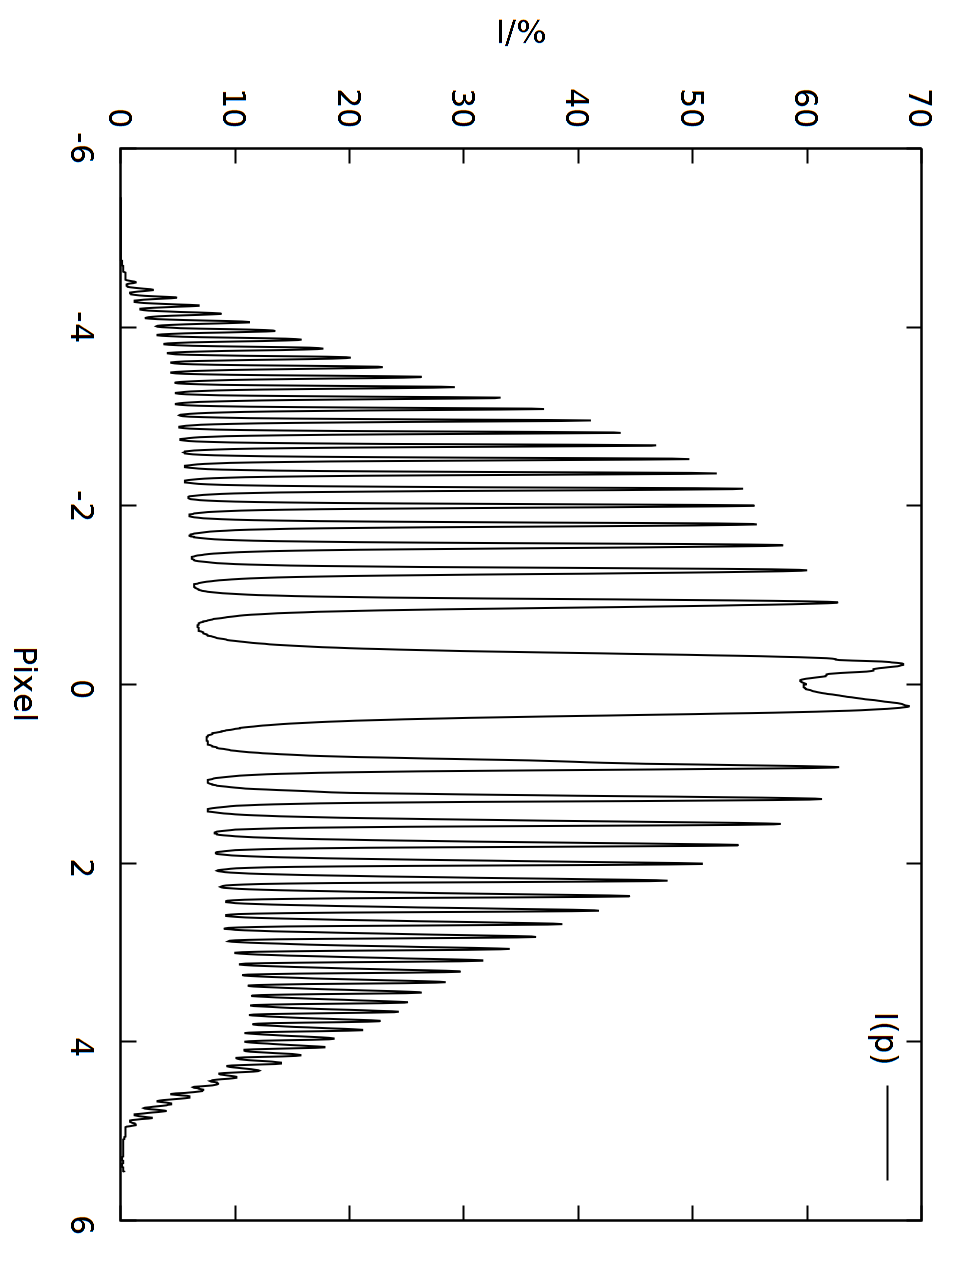
\includegraphics[scale=0.25]{data/zeeman/out_0_0_raw.png}
\caption{Interferenzmuster ohne Magnetfeld}
\label{fig:ohneb}
\end{figure}

$\Delta \lambda$ ergibt sich nun aus dem Unterschied der Gangunterschiede, $\delta \lambda$ aus dem Unterschied der Gangunterschiede beim Maximum des Peaks und bei der Halbwertsbreite.
\begin{align*}
F = \frac{\Delta \lambda}{\delta \lambda} &= \frac{2d}{2d}\frac{\sqrt{n^2-\sin^2(\alpha_1)}-\sqrt{n^2-\sin^2(\alpha_2)}}{\sqrt{n^2-\sin^2(\alpha_1+\delta \alpha)}-\sqrt{n^2-\sin^2(\alpha_1)}}\\
	&= \frac{(675 \pm 8) \si{\nano\meter}}{(54 \pm 6) \si{\nano\meter}}\\
	&=12,5 \pm 1,4
\end{align*}
Dieser Wert ist etwas zu groß, aber trotzdem in der gleichen Größenordnung. Wir vermuten, dass der Unterschied möglicherweise dadurch gegeben ist, dass wir die Peaks nicht über einen Fit bestimmt haben, sondern einfach abgelesen haben. Da die Kurve ein Überlagerung verschiedener Gausskurven ist, werden die Werte leicht verschoben.

\paragraph{Dopplerverbreiterung}
Die Dopplerverbreiterung ergibt sich durch ($m = 112,4\si{\atomicmassunit}$ \cite{wiki_cd}, $ T = 1000\si{\kelvin}$ angenommen):
\begin{align*}
\delta \lambda\ind{Doppler} &= \frac{\lambda}{c}\sqrt{\frac{3k\ind{B}T}{m}}\\
&= 0,001029 \si{\nano\meter}
\end{align*}
Dieser Wert ist deutlich kleiner als die Breite des mittleren Peaks (siehe letzten Abschnitt) $(54 \pm 6) \si{\nano\meter}$. Die Dopplerverbreiterung kann man also in diesem Experiment vernachlässigen.
